% !Mode:: "TeX:UTF-8"
% !TEX builder = LATEXMK
% !TEX program = xelatex
\documentclass[master,twoside,nocpsupervisor]{zjuthesis}

% 插图路径设置,图片放在figures 文件夹下。一般来说论文的插图比较多,通常按章节存
% 放,因此可以在以下命令中在按章节添加存放图片的文件夹路径。如以下这个路径中 ./
% 代表当前main.tex所在的目录,就是一般所说的当前文件夹;figures 文件夹就是子文件
% 夹,存放正文及附录中要用到的所有的图片,在figures 文件夹中的子文件夹就是存放各
% 个章节图片的文件夹,一般命名与相应章节的名字相同,如intro 章节用到的图片全放在
% 了intro 这个子文件夹下。
\graphicspath{%
	{./figures/intro/}%
}

% 论文中文标题
\title{模态不匹配下的非线性Markov跳变系统控制问题}
% 论文英文标题
\englishtitle{Studies on Nonlinear Markov Jump Systems with Mismatch Modes}
% 作者,就是你的名字
\author{ 陶跃跃}
% 分类号
\classification{TM863}
% 单位代码
\serialnumber{10335}
% 密级
\secretlevel{公开 }
% 学号
\studentnumber{21732013}
% 指导教师
\supervisor{吴争光}
% 合作导师,如果没有合作导师,就在\documentclass选项栏中加上"nocpsupervisor"。
\cpsupervisor{庞统}
% 专业名称
\major{控制科学与工程}
% 研究方向
\research{随机系统控制理论}
% 所在学院
\institute{控制科学与工程学院}
% 提交日期
\submitdate{2020年1月1日}

% 中文题名页
\reviewerA{ \hspace{1.5em} \hspace{1.5em}  }
\reviewerB{ \hspace{1.5em} \hspace{1.5em} }
\reviewerC{ \hspace{1.5em} \hspace{1.5em}  }
\reviewerD{ \hspace{1.5em} \hspace{1.5em}  }
\reviewerE{ \hspace{1.5em} \hspace{1.5em}  }
\chairperson{ \hspace{1.5em} \hspace{1.5em}  }
\commissionerA{ \hspace{1.5em} \hspace{1.5em}  }
\commissionerB{ \hspace{1.5em} \hspace{1.5em}  }
\commissionerC{ \hspace{1.5em} \hspace{1.5em}  }
\commissionerD{ \hspace{1.5em} \hspace{1.5em}  }
\commissionerE{ \hspace{1.5em} \hspace{1.5em}  }
\defencedate{ }

% 英文题名页
\enreviewerA{ \hspace{1.5em}   \hspace{1.5em}  }
\enreviewerB{ \hspace{1.5em}   \hspace{1.5em}  }
\enreviewerC{ \hspace{1.5em}   \hspace{1.5em}  }
\enreviewerD{ \hspace{1.5em}   \hspace{1.5em}  }
\enreviewerE{ \hspace{1.5em}   \hspace{1.5em}  }
\enchairperson{ \hspace{1.5em}   \hspace{1.5em}  }
\encommissionerA{ \hspace{1.5em}   \hspace{1.5em}  }
\encommissionerB{ \hspace{1.5em}   \hspace{1.5em}  }
\encommissionerC{ \hspace{1.5em}   \hspace{1.5em}  }
\encommissionerD{ \hspace{1.5em}   \hspace{1.5em}  }
\encommissionerE{ \hspace{1.5em}   \hspace{1.5em}  }
\eendefencedate{  }

\begin{document}
\maketitle
% \ZJUmakecover
% \ZJUmakeCNtitlepage
% \ZJUmakeENtitlepage
\frontmatter
% !TEX root = ../thesis.tex
\chapter{致\texorpdfstring{\ZJUspace}{}谢}
岁月如梭,转眼间,X年的XX生求学生活即将结束,站在毕业的门槛上,回首往昔,奋斗和辛劳成为丝丝的记忆,甜美与欢笑也都尘埃落定。浙江大学以其优良的学习风气、严谨的科研氛围教我求学,以其博大包容的情怀胸襟、浪漫充实的校园生活育我成人。值此毕业论文完成之际,我谨向所有关心、爱护、帮助我的人们表示最诚挚的感谢与最美好的祝愿。

本论文是在导师诸葛亮丞相的悉心指导之下完成的。三年来,导师渊博的专业知识,严谨的治学态度,精益求精的工作作风,诲人不倦的高尚师德,朴实无华、平易近人的人格魅力对我影响深远。导师不仅授我以文,而且教我做人,虽历时X载,却赋予我终生受益无穷之道。本论文从选题到完成,几易其稿,每一步都是在导师的指导下完成的,倾注了导师大量的心血,在此我向我的导师诸葛丞相表示深切的谢意与祝福!


本论文是在导师诸葛亮丞相的悉心指导之下完成的。三年来,导师渊博的专业知识,严谨的治学态度,精益求精的工作作风,诲人不倦的高尚师德,朴实无华、平易近人的人格魅力对我影响深远。导师不仅授我以文,而且教我做人,虽历时X载,却赋予我终生受益无穷之道。本论文从选题到完成,几易其稿,每一步都是在导师的指导下完成的,倾注了导师大量的心血,在此我向我的导师诸葛丞相表示深切的谢意与祝福!


本论文是在导师诸葛亮丞相的悉心指导之下完成的。三年来,导师渊博的专业知识,严谨的治学态度,精益求精的工作作风,诲人不倦的高尚师德,朴实无华、平易近人的人格魅力对我影响深远。导师不仅授我以文,而且教我做人,虽历时X载,却赋予我终生受益无穷之道。本论文从选题到完成,几易其稿,每一步都是在导师的指导下完成的,倾注了导师大量的心血,在此我向我的导师诸葛丞相表示深切的谢意与祝福!

本论文的完成也离不开其他各位老师、同学和朋友的关心与帮助。在此也要感谢关羽、赵云等各位老师在论文开题、初稿、预答辩期间所提出的宝贵意见,感谢木牛流马课题组为本论文提供的数据和建议,还要感谢同门的师兄师妹们,在科研过程中给我以许多鼓励和帮助。回想整个论文的写作过程,虽有不易,却让我除却浮躁,经历了思考和启示,也更加深切地体会了法学的精髓和意义,因此倍感珍惜。

还要感谢父母在我求学生涯中给与我无微不至的关怀和照顾,一如既往地支持我、鼓励我。同时,还要感谢关某某同学、赵某某同学、张某某同学、黄某某同学X年来对我的爱护、包容和帮助,愿友谊长存!

\vspace{2cm}
\hfill
\begin{minipage}{14em}
\begin{center}
于XX地\quad 225年1月1日\\
我的名
\end{center}
\end{minipage}

% !TEX root = ../thesis.tex

% 定义中文摘要和关键字
\begin{cabstract}
	传统的Markov跳变系统理论大多基于控制器模态同系统模态完全一致这一完美假设。但在实际应用中,由于通信系统在可靠性、性能等方面的限制,可能会出现系统模态信息丢失、传输延迟等现象,使得控制器不能获取正确的系统模态;模态切换装置的故障、切换效率低也可能使得控制器不能及时的切换到对应的系统模态。上述两个因素都会导致控制器的模态可能会同系统模态不一致,出现模态不匹配现象。学者们提出了隐Markov模型来处理这种模态不匹配问题,模型基于统计学规律,推测控制器可能的模态,降低了对通讯、切换等物理条件的要求,更加符合实际应用场景。同时,该模型可以通过调整模态转移概率矩阵,分别应对模态完全匹配、模态部分匹配、模态完全不匹配这三种情况,是一个强大的统一模型。非线性系统是非常常见的控制系统,在本文中,我们将针对几类典型的非线性Markov跳变系统,研究其模态不匹配控制问题。
	
	本文主要内容可以总结如下:
	
	(1) 针对一类Markov跳变Lur'e系统,考虑到控制器模态同系统模态可能存在不匹配的情况,我们引入了隐Markov模型来设计了一个由一个线性状态反馈和一个同系统非线性保持一致的非线性输出反馈组成的异步控制器,复合控制器结构相比单状态反馈控制器更加灵活,控制效果更好;同时,讨论了系统的稳定性及$l_2$性能,得到了一个LMI形式的充分条件,使得系统随机稳定的同时保证了一定$l_2$性能。使用了一个例子验证了异步控制器的有效性,同时探究了条件转移概率、控制器异步率、最优$l_2$性能之间的关系。
	
	(2) 研究了一类Roesser模型下的非线性二维(2D)Markov跳变控制系统的异步滑模控制问题。考虑到2D系统的特性,首先构造了一个新颖的2D滑模面,同时考虑到控制器模态同系统模态的不匹配情况,基于构造的滑模面、隐Markov模型设计了一个异步2D滑模控制器。先是分别讨论了在此异步滑模控制器作用下系统的稳定性、$H_\infty$性能及系统状态到滑模面的可达性问题,然后得到了一个能够保证一定$H_\infty$性能且稳定的同时,保证系统状态可达性的充分条件。 并根据得到的结果提出了一个异步2D滑模控制器设计算法,最终使用数值仿真例子验证了该算法的有效性。
	
	(3) 研究了Roesser模型下2D-Markov跳变系统的异步二次型控制问题。 考虑到控制器模态同系统模态的不匹配情况,基于隐Markov模型设计了一个异步线性状态反馈控制器。 定义了一个二次型成本函数,并分别讨论了三种不同的初始条件下系统的稳定性和保成本性能。根据初始条件情况的不同,分成了三种情况进行讨论
		\begin{itemize}
			\item 系统初始状态、初始模态都已知;
			\item 系统初始状态有界、初始模态已知;
			\item 系统初始状态有界、初始模态未知;
		\end{itemize}
	最终,我们得到了使得系统系统的充分条件,并得到了不同初始条件下的保成本性能。
	

  
\end{cabstract}

\ckeywords{Markov跳变系统; 模态不匹配;异步控制; 隐Markov模型; Lur'e系统; 2D系统}

% !TEX root = ../thesis.tex

% 定义英文摘要和关键字

\begin{eabstract}
Most results of Markov jump systems are based on a implicit assumption, that is, the modes of controller are the same as modes of original system. However, the imperfection of  physical devices might impair this ideal assumption. On the one hand, the controller may will not receive accurate system modes information due to package loss or delays. On the other hand, failure of the mode switching devices and low stitching efficiency may also prevent the controller from  timely switching to the corresponding system mode. Researchers proposed a  statistical method called hidden Markov model, which weaken the needs of physical devices and more practical compared with absolute match case, to deal with the modes mismatch problem. In this model, the controller modes are obtained by a conditional transition probability from modes of system to controller. We can handle all match, partial match, none match of modes between controller and system simultaneously by adjust the conditional transition probability, which means the hidden Markov model is a powerful unite model. In this paper, we will discuss the control problems of some classic nonlinear Markov jump systems with mismatch modes.

The main contributions are list as follows

(1) Considering a class of Markov jump Lur'e systems with mismatch modes information,  we design a asynchronous controller which is composed of  linear state feedback and  nonlinear (the same as system) output feedback, based on hidden Markov model.  The unique controller structure is more flexible  than the  state feedback ones and will have better results. Then, the stability and $l_2$ performance are discussed, a sufficient condition presented in LMI is obtained to guarantee the system is stochastically stable with a $l_2$ performance from disturbance to output. Finally, a numerical example is provided to illustrate the effectiveness of obtained results.

(2) Considering a class of nonlinear 2D-Markov jump systems in Rosser model, we study the sliding mode control problems of it. Noting the special properties of 2D systems, a novel 2D sliding surface is constructed. In order to handle the mismatch modes between system and controller, the hidden Markov model is introduced to design the sliding mode control law. Then, we discuss the system stability with a  $H_\infty$ performance and the reachability of states to the sliding surface, respectively. A sufficient condition is obtained which can guarantee the system is  asymptotically mean square stable with a $H_\infty$  performance and the reachability of sliding mode dynamics, simultaneously. Finally, we summaries  the sliding mode controller design procedures into to an algorithm whose effectiveness is verified by a numerical example. 


(3) Considering a class of 2D-Markov jump systems in Rosser model, we study the quadric control problems of it. Noting the mismatch modes between controller and system, we introduce a hidden Markov model to design a asynchronous state feedback controller. Then, a quadric cost function is defined and the system stability is discussed. The guaranteed cost performance is studied based on three different initial conditions
 
 \begin{itemize}
 	\item  both initial system states  and initial system modes are known,
 	\item  initial system states satisfy a bounded condition and initial system modes are known,
 	\item  initial system states satisfy a bounded condition and initial system modes are known.
 \end{itemize}
 Finally,  sufficient conditions that can make sure system is stable with a optimal guaranteed cost performance  of different initial conditions are obtained.


\end{eabstract}

\ekeywords{Markov jump systems, mismatch modes, asynchronous control,hidden Markov model, Lur'e systems, 2D systems}

% 正文目录:
\tableofcontents
% 插图目录:
\listoffigures
% 表格目录:
%\listoftables
% !TEX root = ../thesis.tex
\begin{denotation}
\item[$T$]  表示单位矩阵
\item[$\mathbb{R}^{n}$]  表示$n$维实向量集合
\item[$\mathbb{R}^{m\times n}$]  表示$m\times n$维实矩阵集集合
\item[$\mathbb{E}\{\cdot \}$]  表示数学期望运算
\item [$\Pr\{X\}$]  表示事件$X$发生的概率
\item [$\Pr\{Y|X\}$]  表示在事件$X$前提下,事件$Y$发生的条件概率
\item [$X^{-1}$] 表示矩阵$X$的逆
\item [$X^{T}$] 表示矩阵$X$的转置
\item [$X>0(X\geq 0)($] 表示矩阵$X$为正定(半正定)矩阵
\item [$\lambda_{max}(X)$] 表示矩阵$X$的最大特征值
\item [$\lambda_{min}(X)$] 表示矩阵$X$的最小特征值

\item [$\|x\|$] 表示向量$x$的2-范数
\item [$\|X\|$] 表示矩阵$X$的谱范数
\item [$\mathrm{diag}\{X_1,X_2,\dots,X_n \}$]  表示对角元素为$X_i(i=1,2,\dots,n)$的对角矩阵

\item [LMI]  表示线性矩阵不等式 

\end{denotation}

\mainmatter
% !TEX root = ../thesis.tex

\chapter{绪论}
\section{引言}
	在实际工程应用中,由于种种因素,如信息传输丢失、外部环境突变、子系统连接变化等,可能会导致系统结构、参数的变化。为了描述这种现象,学者们提出了Markov模型来对这类系统进行建模,并称这类系统为Markov跳变系统。近年来,由于Markov跳变系统对上述现象的强大建模能力获得了广泛而深入的研究。同时,非线性是控制系统中最常见的一类现象,在众多的非线性类别中,有一种非线性因其广泛存在及独特的性质,学者们对其进行了专门而系统的研究,并称之为Lur'e系统。由于一些应用,如一个房间内的温度、湿度随着空间、时间的变化规律,使用一维(1D)系统模型难以建模或模型不够精确,因而学者们提出了能更加精确建模的二维(2D)控制系统模型。在本文中,我们将围绕Markov跳变Lur'e系统、2D-Markov跳变系统展开讨论。在本章,我们重点介绍Markov跳变系统及研究现状,给出阅读本文需要的预备知识背景并介绍本文的研究内容。而Lur'e系统、2D系统及相关的控制概念,我们将在稍后的相关章节中作进一步的详细介绍。

\section{Markov跳变系统}
	Markov跳变系统实际上是一种特殊的基于统计学的切换系统。当系统的结构、参数发生变化时,我们认为系统由某个子系统切换到了另一个子系统,同时我们使用模态来表示这若干个子系统。根据这样的假设,不难发现,系统有多少种不同的结构、参数,就应该有多少个子系统,对应同等数量的系统模态。同其他切换系统不同的是,Markov跳变系统模态之间的切换是由一个Markov链来控制的,即模态切换遵循Markov过程。一个简单的离散Markov跳变系统\eqref{intro-system-eq}可以表示为,
	\begin{equation}\label{intro-system-eq}
		x(k+1)=A(r(k))x(k)+B(r(k))u(k)
	\end{equation}
	这里$\{r(k),k\geq 0 \}$表示系统模态对应的Markov链,在集合$\{1,2,\dots,N \}$中取值,$N$表示系统的模态数量。人们通过对系统模态进行统计,得到模态间的切换规律,并将其表示为具有如下形式的模态转移概率
	\begin{equation}\label{introduction-tps-sys}
	\Pr\{r(k+1)=j|r(k)=i \}=\pi_{ij}
	\end{equation}
	因此,一般来说,系统在下一个时刻的模态可以由当前模态通过模态转移概率推测得到。一个简单具有$N$个模态的Markov跳变系统可以用图\ref{intro_system}表示。
	\begin{figure}[!htb] 
		\centering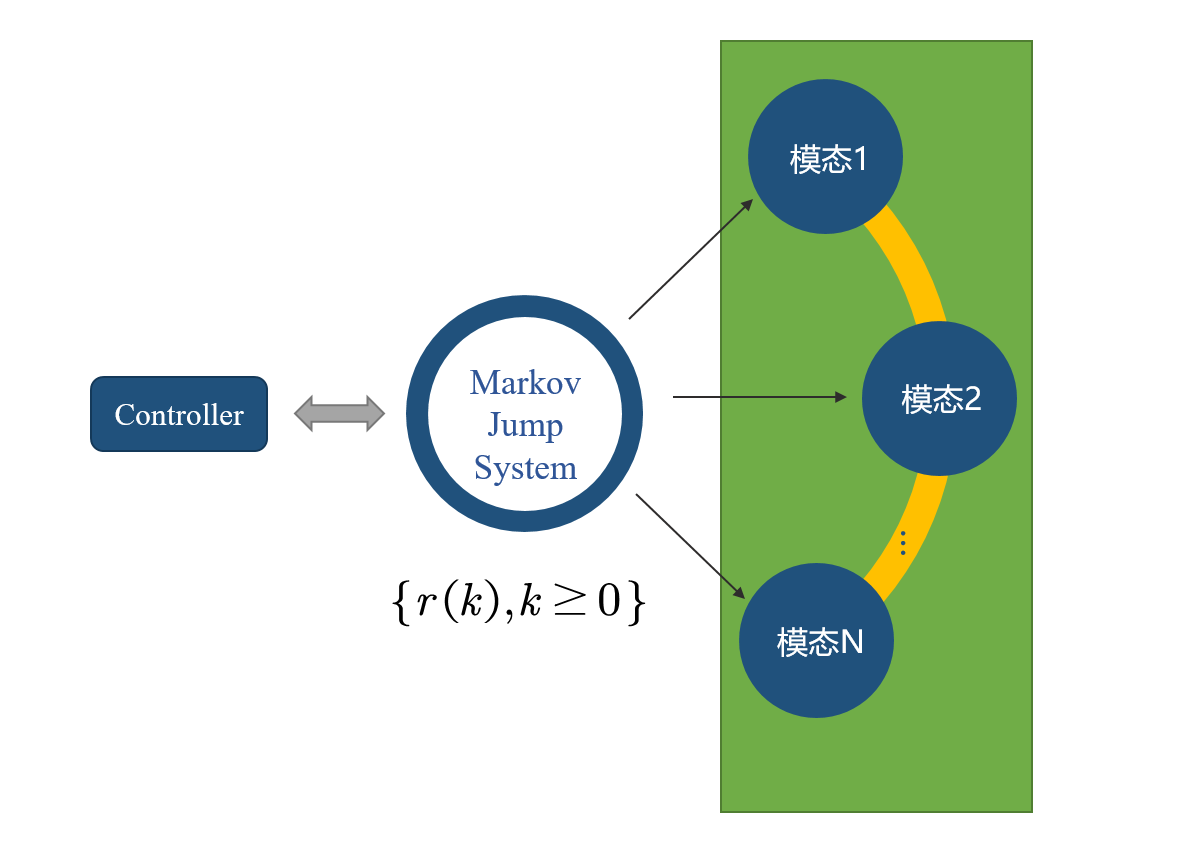
\includegraphics[scale=0.25]{./figures/introduction/system.png}\\ 
		\caption{Markov跳变系统示意图}
		\label{intro_system}
	\end{figure}

	自Markov跳变系统首次提出以来\cite{florentin1961optimal},便取得了国内外学者们的广泛关注,并取得了众多理论研究成果\cite{costa2006discrete,de2000output,xiong2005robust,ma2010stability,zhang2009hestimation,xu2007delay}。同时,Markov跳变控制系统已经成功的应用到金融分析系统\cite{mamon2007hidden}、 故障检测\cite{zhong2005faultdetection}、网络通讯\cite{network-communication-kim2004}、飞行器控制\cite{bar1993estimation,gray2000stability}、机器臂\cite{goncalves2004nonlinear}等实际应用中。近年来,Markov跳变系统取得了诸多突破性的进展。例如,针对模态转移概率可能没有实现得到(模态转移概率不确定)的情况,文献\cite{zhang2009stability}提出了系统模态转移概率部分已知的控制方法,该方法涵盖了模态转移矩阵完全已知、完全未知的情况,并且利用该方法对连续、离散线性Markov跳变系统的稳定性进行了分析。之后,一些学者将该方法分别推广到了$H_{\infty}$控制\cite{luan2012h}、$H_\infty$滤波\cite{ma2009robust}、奇异系统\cite{kao2014stabilization}等。另一方面,先前对Markov跳变系统的控制、滤波问题的研究大多基于控制器模态能够同系统模态同步切换这一假设。而在现实控制系统中,由于通讯系统的可靠性及性能并不完美,可能会导致控制器难以检测到系统当前所处的模态;而且想要让控制器模态与系统模态同步切换,对控制器模态切换装置的可靠性、效率也有很高的要求。在文献\cite{do2014detector}中,提出了基于检测的控制器设计方法,该方法认为系统中存在一个装置能够检测系统的模态信息,并按照一个统计学规则来推测控制器的模态。文献\cite{zhang2009stability}假设控制器的模态会滞后于系统的模态,并提出了异步控制的概念。文献\cite{wu2016passivity}研究了基于隐Markov模型的异步无源控制问题,在本文中,控制器的模态会由系统模态通过一个条件概率求得。上述文献,分别从不同的角度对同一个问题进行了阐述,即控制器模态同系统模态不匹配问题。随后,学者们使用隐Markov模型来处理模态信息不匹的$H_\infty$控制、$H_\infty$滤波、无源控制、模型推导、故障检测、多智能体控制等问题进行了研究。下面我们将按照系统模态同控制器模态的匹配角度,对Markov跳变系统的控制问题进行进一步的阐述。

\section{模态信息不匹配控制}
	目前,根据控制器模态同系统模态的匹配情况,可以将Markov跳变系统的控制器分为三类:模态独立控制器、模态同步控制器、异步控制器。下面我们将针对这三类控制器分别展开讨论。
	\subsection{同步控制器}
	同步控制器对应的是模态信息完全匹配的情况。一般来说,控制器应该有如下形式,
	\begin{equation}
		u(k)=K(r(k))x(k)
	\end{equation}
	这不难发现,这里控制器的模态和系统的模态都是使用$r(k)$来表示的,也就是说控制器的模态应该同系统模态保持一致,即控制器模态同系统模态完全匹配。最早关于Markov跳变系统的研究都假设控制器的模态是和系统模态保持一致的,并且取得了众多的研究成果。一般而言,模态完全匹配的情况,在系统分析上比较简单,同时,得到的结果也会比其他两种情况要好一些。但是,在实际控制系统中,控制器模态想要同系统模态始终保持一致是非常困难的。首先,由于在网络传输过程中存在信息丢失的情况,控制器可能在某些时刻获取不到系统模态信息。其次,由于网络传输存在延迟,控制器可能得到的是先前时刻的系统模态信息,而此时系统已经切换到另外一个模态,进而导致控制器模态同系统模态不匹配。另外,即使控制器及时的得到了当前时刻精确的系统模态信息,但是由于物理因素的限制,控制器可能不能及时的切换到对应模态,即控制器模态切换速度跟不上系统模态切换速度,进而又出现了模态不匹配的情况。就是说,如果想要实现模态信息始终匹配,我们需要拥有一套可靠、高性能的通讯系统和模态切换装置。显然,这个要求是非常苛刻的。因此,同步控制器设计尽管分析起来非常简单,却有些不太符合实际情况了。
	
	\subsection{模态独立控制器}
	模态独立控制器对应的是模态信息完全不匹配的情况。 一般来说,模态独立控制器应该有如下形式,
	\begin{equation}
	u(k)=K(q(k))x(k)
	\end{equation}
	这里,$q(k)$表示控制器在$k$时刻的模态,可能在集合$\{1,2,\dots,M \}$中取值,但是服从另外一个独立的Markov过程,其状态转移概率为
	\begin{equation}\label{introdution-tps-indp} 
	\Pr\{q(k+1)=j|q(k)=i \}=\lambda_{ij}
	\end{equation}
	由\eqref{introdution-tps-indp}可以推断,对模态独立控制器的情况,当前时刻的控制器模态只跟上一个时刻的控制器模态有关,同系统模态没有任何关系,即控制器模态同系统模态完全不匹配(注意,本文中,完全不匹配并不是指控制器模态始终同系统模不一致,而是两者之间不存在联系的意思)。图\ref{intro_fig_idpsys}表示了一个简单的模态独立控制器作用下的Markov跳变系统。目前,文献\cite{todorov2016new,wu2005mode,dolgov2017static}对模态独立Markov控制问题展开了研究,并得到了相应的结果。值得注意的是,当我们施加了$M=N$,$\lambda_{ij}=\pi_{ij}$,$r(0)=p(0)$这三个限制条件后,似乎控制器变成了模态完全匹配(同步)的情况,但本质上却并不是同步控制器。一个简单的理解为,假设$k$时刻系统模态和控制器模态是一样的,但是由于控制器和系统在$(k+1)$时刻的模态都是由概率(此时概率一样)求得的,因此也可能模态不一致;在同步控制器里,控制器在$(k+1)$时刻的模态是通过检测$(k+1)$时刻系统模态得到的。对于模态独立控制器,不难发现控制器完全没有使用到系统的模态信息,这可能导致的结果是,一方面得到的结果会比较保守;另一方面,对实际应用也没有什么太大的意义。
	
	\begin{figure}[!htb] 
		\centering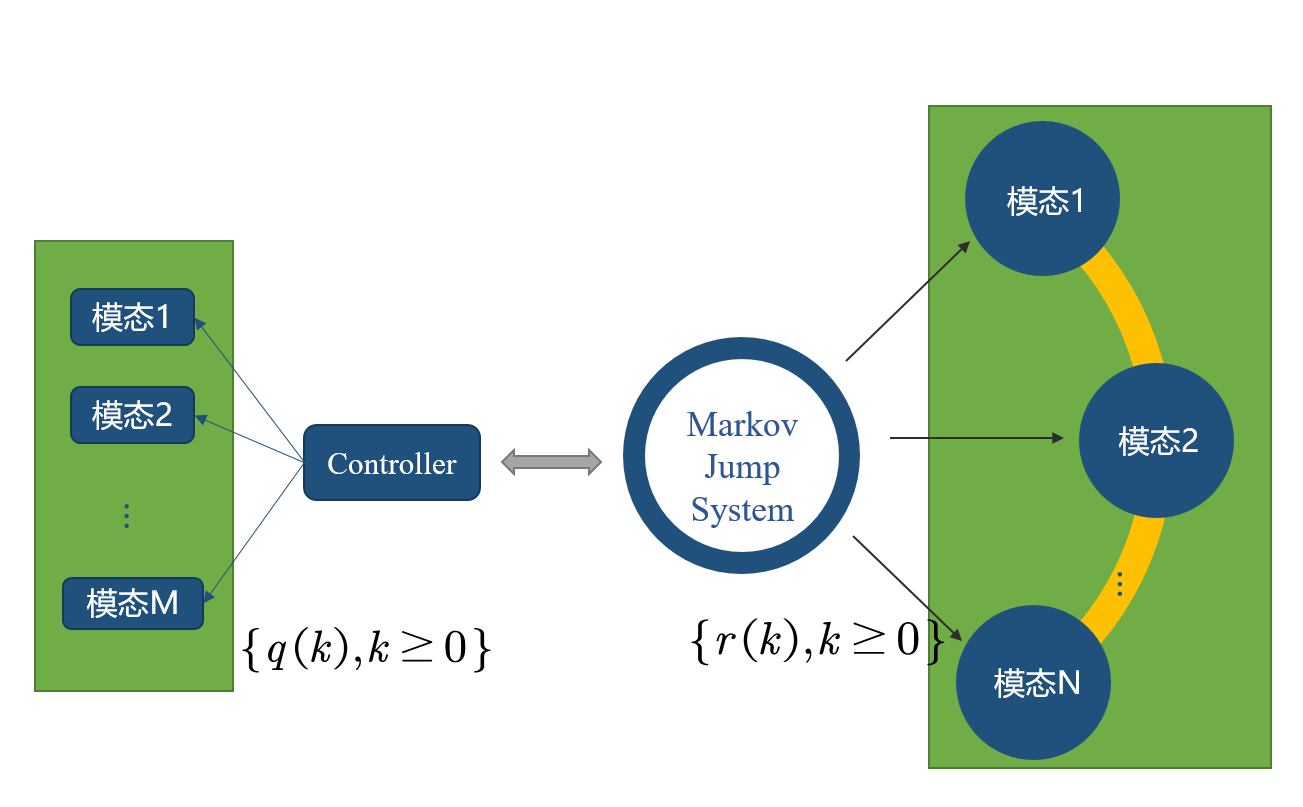
\includegraphics[scale=0.25]{./figures/introduction/idpsys.png}\\ 
		\caption{模态独立控制器作用下的Markov跳变系统}
		\label{intro_fig_idpsys}
	\end{figure}
	
	\subsection{异步控制器}
	模态独立控制器对应的是模态信息不完全匹配的情况。 一般来说,基于隐Markov模型的异步控制器应该有如下形式,
	\begin{equation}
	u(k)=K(\sigma(k))x(k)
	\end{equation}
	这里,$\sigma(k)$表示控制器在$k$时刻的模态,可能在集合$\{1,2,\dots,M\}$中取值,服从一个满足如下条件模态转移概率的随机跳变过程,
	\begin{equation}\label{introdution-tps-asyn}
	\Pr\{\sigma(k)=\phi|r(k)=i \}=\mu_{i\phi}
	\end{equation}
	由\eqref{introdution-tps-asyn}我们可以发现,控制器在$k$时刻的模态是由$k$时刻的系统模态和条件概率推测的。对比同步控制器,我们可以理解同步控制器为$\mu_{ii=1}$的情况。也就是说,对同步控制器而言,$k$时刻系统模态是多少,控制器的模态就应该是多少。 而对异步控制器而言,$k$时刻控制器的模态却是通过条件概率求得的,并不一定同系统模态保持一致。对比模态独立控制器,$k$时刻模态独立控制器的模态是由前一时刻($k-1$)推测的,根本就没有利用任何时刻系统的模态信息。那么,我们发现,下面几个结论(异步控制器的优点)
		
		(1) 异步控制器通过调整条件概率转变成同步控制器,
		
		(2) 异步控制器不需要严格要求控制器模态同系统模态保持一致,更符合实际情况,
		
		(3) 同模态独立控制器相比,异步控制器利用了更充分的系统信息,得到的结果更加有价值。
		
		结论(1)是比较直观的。我们重点讨论一下结论(2),这里需要注意的是,相对于同步控制器,异步控制器削弱了对同步控制器三个完美前提的依赖, 即:一定能获得系统的模态信息、系统模态信息获得足够及时、控制器在获得系统模态信息后能马上切换。异步控制器,对于上述三个前提假设,并没有采用什么优秀的改进方法来改善它们,而是正视这些不完美的存在。控制器通过一个检测器预先采集足够多的信息,统计模态间的切换规律,来推断当前控制器所处的模态。因此,在许多文章中,又称异步控制器设计方法为基于检测器的控制器设计方法。另一方面,前文中已经说过,本文研究的异步控制器是基于隐Markov模型设计的,因此这样的控制器可以涵盖同步、异步、模态独立(单模态)这三种情况,是一个比较综合的控制器设计方法。
		
		由上述可知,基于隐Markov模型的异步控制器在处理模态不匹配的场景下具有诸多优势。因此,在本文中,我们将采用该模型来设计异步控制器,进而对系统的稳定性及各种性能进行分析。
	
	\begin{figure}[!htb] 
		\centering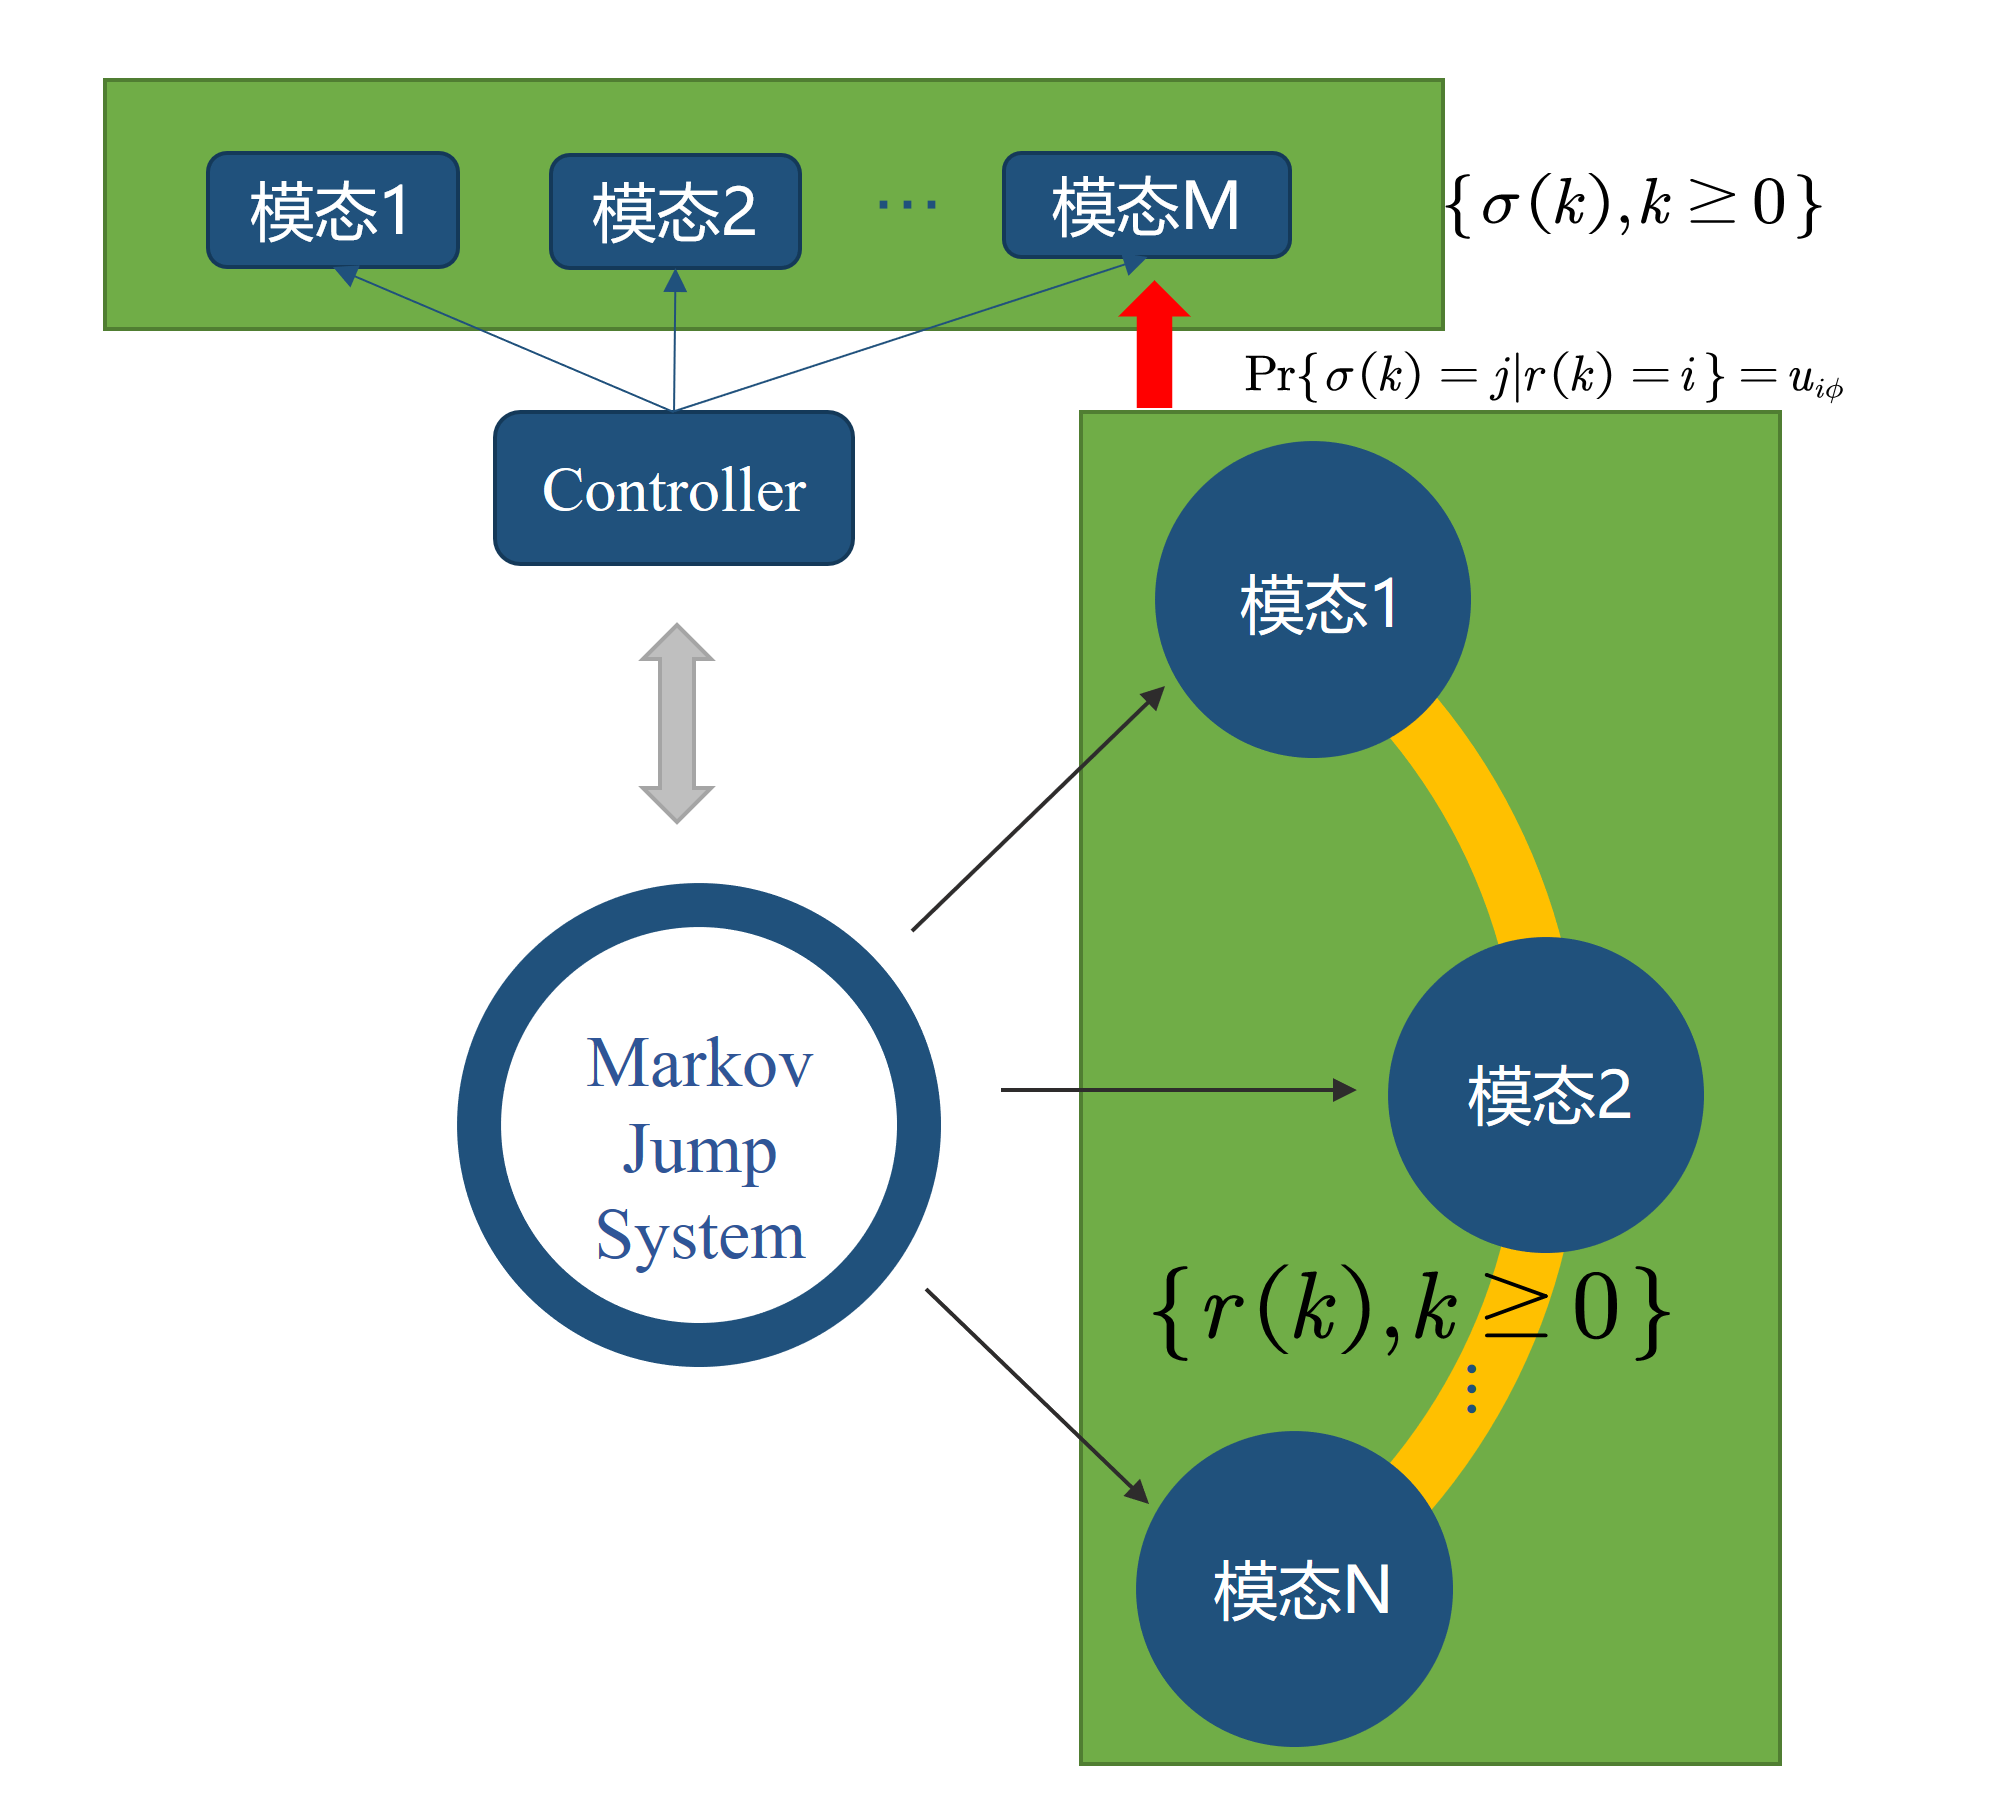
\includegraphics[scale=0.12]{./figures/introduction/asynsys.png}\\ 
		\caption{异步控制器作用下的Markov跳变系统}
		\label{intro_fig_asynsys}
	\end{figure}
	
\section{预备定理}
	本文中,我们将尽量将最终结果以LMI的形式呈现,因此需要使用到Schur补引理将普通的非线性不等式转换为LMI。
	
	{\bf 引理 \ \ 1.1:}(Schur补引理\cite{boyd1994linear}) 若存在实对称矩阵$S_{11}\in\mathbb{R}^{n\times n}$,$S_{22}\in\mathbb{R}^{m\times m}$,矩阵$S_{12}\in\mathbb{R}^{n\times m}$,那么下面三个条件是互为等价的:
	\begin{equation}
		\begin{bmatrix}
			S_{11}&S_{12}\\
			*&S_{22}
		\end{bmatrix}<0,
	\end{equation} 
	\begin{equation}
		S_{11}<0,S_{22}-S^{T}_{12}S^{-1}_{11}S_{12}<0,
	\end{equation} 
	\begin{equation}
		S_{22}<0,S_{11}-S^{T}_{12}S^{-1}_{22}S^{T}_{12}<0.
	\end{equation} 
		
\section{本文的研究内容}
	由于诸如信息传输丢失、外部环境突变、子系统连接变化等因素的影响,会导致系统结构、参数的突变,学者们使用Markov系统来对这类现象进行建模,并在过去的几十年里取得了许多重要的成果。另一方面,非线性广泛的存在实际控制系统中,因此非线性Markov跳变系统也是一种非常重要的控制系统。目前大多数对非线性Markov跳变系统的研究都基于控制器模态同系统模态这一严格的假设。 但是由于这一假设对通讯、切换等物理装置的要求过于苛刻,因此尽管取得的成果非常优秀,却并不能在实际应用中进行广泛推广。隐Markov模型削弱了该假设的严格要求,同时充分利用了系统信息,是一个优秀的包含模态完全匹配、模态部分匹配、模态完全不匹配的统一模型。本文中将基于隐Markov模型来设计异步控制器,对非线性Markov跳变系统的稳定性,$l_2$、$H_\infty$、保成本等性能进行研究。主要工作归纳如下:
	
	(1) 在第二章中,考虑到Lur'e系统在实际应用中的普遍性及在非线性系统中的重要地位,我们对一类Markov跳变Lur'e系统展开了研究。首先考虑到控制器模态同系统模态可能存在不匹配的情况,我们引入了隐Markov模型来设计异步控制器;该控制器由一个线性状态反馈和一个非线性输出反馈组成,这个非线性环节同Lur'e系统的非线性是一样的,都满足一个有限扇形条件,这样的控制器结构可以使得我们得到的结果相比只有状态反馈的结构得到的结果更加不保守;随后,我们对这类Markov跳变Lur'e系统的稳定性及$l_2$性能进行了研究,得到了满足一定$l_2$性能同时保证系统随机稳定的充分条件。最后,我们使用了一个例子验证了异步控制器的有效性,同时探究了条件转移概率、控制器异步率、最优$l_2$性能之间的关系。
	
	(2) 在第三章中,我们研究了一类Rosser模型下的非线性二维Markov跳变控制系统的滑模控制问题。考虑到2D系统的特殊结构相比1D系统给系统分析带来了更多的复杂性和困难,我们构造了一个新颖的2D滑模面。同时考虑到控制器模态同系统模态的不匹配情况,基于构造的滑模面,引入隐Markov模型设计了一个2D异步滑模控制器。我们首先研究了在此异步滑模控制器下系统的稳定性及$H_\infty$性能问题,得到了能够使得系统满足一定$H_\infty$性能同时保证渐进均方稳定的充分条件;同时,我们又研究了系统状态到滑模面的可达性问题,得到了一个可以使得系统状态到达滑模面某个领域内部的充分条件;然后,我们在上述两个结果的基础上,给出了能够保证一定$H_\infty$性能且稳定的同时,保证系统状态可达性的充分条件。随后,我们把本章结果进行归纳,得到了一个2D异步滑模控制器设计算法。最后,我们使用了一个数值仿真例子来验证2D异步滑模控制的有效性。
	
	(3) 在第四章中,我们研究了Rosser模型下二维Markov跳变系统的二次型控制问题。首先,考虑到控制器模态同系统模态的不匹配问题,基于隐Markov模型,我们设计了一个异步线性状态反馈控制器。然后,定义了一个二次型成本函数,并分别讨论了三种不同的初始条件下系统的稳定性和保成本性能问题。相对1D系统,由于2D系统的初始模态和初始状态都不止一个,因此,情况也要更加的复杂,分析起来也更加困难。在本章中,我们把初始条件分为了三类进行讨论。第一种情况是假设初始模态和初始状态都已知,这种情况下,我们对系统的初始信息要求掌握的足够多,但是得到的保成本性能是最好的;第二种情况是假设初始模态已知,全部的初始状态都满足一定的约束条件。此时,我们降低了对系统初始状态信息的要求,但是保成本性能略有下降;第三种情况是系统的初始模态不知道,全部初始状态都满足一定的约束条件。它在第二种情况的基础上进一步降低了对系统初始模态的要求,得到的结果形式是最为简单的,但是保成本性能也是三者里最差的。同时,不管是上述哪一种情况,我们都可以使用同一个条件来保证系统的稳定性。最后,我们同样使用了一个仿真实例来验控制器对系统的影响。
	
	
	
	
	
	
% !TEX root = ../thesis.tex

\chapter{模态不匹配Markov跳变Lur'e系统}
	非线性是控制系统中普遍存在的现象之一。由于非线性的存在可能会严重影响控制系统的工作状态,甚至破坏系统的稳定性,所以研究非线性系统具有重要的意义。上个世纪四十年代,前苏联数学家Lur'e在研究飞行器驾驶技术时,发现了一种用有限或者无线扇形区间约束的非线性,自此Lur'e系统\cite{lurie1957some}进入了人们的视野。一般来说,完整的Lur'e由一个线性环节和一个满足有限、无限扇形区间的非线性环节串联组成\cite{khalil2002nonlinear},如
	\begin{equation}
		\left\{
			\begin{array}{lr}
			x_{k+1}=Ax_k+Bf(y_k),\\
			y_k=Cx_k.
			\end{array}
		\right.
	\end{equation}
	Lur'e系统凭借其普遍存在性、广泛适用性,获得了广大学者们的关注。学者们对其进行了深入的研究并取得了一系列重要的成果\cite{kalman1963lyapunov,park2002stability,suykens1997nonlinear,cao2005synchronization}。特别的,在文献\cite{castelan2006absolute,castelan2008control}中,作者针对分别讨论了连续、离散域Lur'e系统的绝对稳定性问题,并在文中提出了一种新型反馈控制结构,该结构由一个线性状态反馈和同系统非线性保持一致的非线性输出反馈组成。这种结构相对于一般的线性状态反馈控制器会更加的灵活,并且会降低得到结果的保守性。文献\cite{gonzaga2012stability}对离散Markov跳变Lur'e系统的稳定性进行了研究,并提出了一种Lur'e型李雅普诺夫函数,进一步降低了得到结果的保守性。同时,Lur'e系统的研究并没有局限在理论层面,在诸如机器人\cite{mahmoud1994globally,chen1999controlling}、飞行器\cite{leonov2012aircraft}、网络通信\cite{li2006stability}等领域有着实际应用。
	
	Markov跳变Lur'e系统在近年来也取得了一系列重要的理论成果。文献\cite{zhu2015distributed,zhang2017resilient,zhang2015model}分别对Markov跳变Lur'e系统的$H_\infty$滤波、无源控制、模型推导问题进行了研究。文章\cite{gonzaga2014stochastic,song2012stability}对一类控制器饱和非线性的Markov跳变控制系统的稳定性和$l_2$性能进行了研究。文章\cite{wu2012stochastic}对一类具有时变时滞和分段恒定转移概率的奇异Markov跳变Lur'e系统进行了讨论。值得注意的是,上述结果基本上都基于控制器模态同系统模态完全匹配这一完美假设。而对模态不匹配的Markov跳变Lur'e系统的研究成果比较少。在文章\cite{song2018event}中,作者结合了事件触发和隐Markov模型,探究了Markov跳变Lur'e系统的异步滑模控制问题。
	
	本章中,考虑到控制器模态同系统模态不一致的问题,我们将引入隐Markov模型,来研究一类Markov跳变Lur'e系统的异步控制问题,并对系统的稳定性及$l_2$性能进行讨论。

\section{数学模型及问题描述}
	本章考虑如下Markov跳变Lur'e系统:
	\begin{equation}\label{syseq}\left\{
	\begin{array}{lr}
		\begin{split}
			x_{k+1}=A_{r(k)}x_k+F_{r(k)}\varphi(y_k)+B_{r(k)}u_k +E^x_{r(k)}w_,
		\end{split}\\
		\begin{split}
			y_k=C_{r(k)}x_k,
		\end{split}
		\\
		\begin{split}
			z_k= C^z_{r(k)}x_k+G^z_{r(k)}\varphi(y_k)+D^z_{r(k)}u_k+E^z_{r(k)}w_k,
		\end{split}	
	\end{array}\right.
	\end{equation}
	这里,$x_k\in\mathbb{R}^{n_x}$ 表示系统状态, $u_k\in\mathbb{R}^{n_u}$ 表示系统控制输入, $y_k\in\mathbb{R}^{n_y}$ 系统观测输出,$ z_k\in\mathbb{R}^{n_z}$ 表示系统被控输出, $w_k\in\mathbb{R}^{n_w}$ 表示外界扰动。 $A_{r(k)}$, $F_{r(k)}$, $B_{r(k)}$, $E^x_{r(k)}$, $C^z_{r(k)}$,$G^z_{r(k)}$, $D^z_{r(k)}$ 及 $E^z_{r(k)}$ 是已知的实系统矩阵且具备合适维度。
	$\{r(k),k\geq0\}$ 是一个Markov链,且在集合 $\mathcal{N}=\{1,2,\dots,N\}$ 中取值,并且满足如下模态转移概率:
	\begin{equation}
	\Pr\{r(k+1)=j|r(k)=i\}=\pi_{ij},
	\end{equation}
	其中,对任意的 $i,j\in\mathcal{N}$,有$\pi_{ij}\in[0,1]$, 且对任意的模态 $i$, 有$\sum_{j=1}^{N}\pi_{ij}=1$。 在$i$ 时刻的系统矩阵可以记作 $A_i$,$F_i$,$B_i$,$E^x_i$,$C^z_i$,$G^z_i$,$D^z_i$,且相应的模态转移矩阵记作 $\varPi=\{\pi_{ij}\}$。
	
	首先,我们对Lur'e系统中的非线性 $\varphi(\cdot)$ 做如下的假设
	
	{\bf 定义 \ \ 2.1:} 
	非线性 $\varphi(\cdot): \mathbb{R}^{n_y}\rightarrow\mathbb{R}^{n_y}$ 符合一个由下面两个条件同时约束的有界扇形条件
		
		(1) $\varphi(0)=0$;
		
		(2) 存在正定矩阵 $\varOmega \in\mathbb{R}^{n_y\times n_y}$,对任意的 $y\in\mathbb{R}^{n_y}$, $\nu \in\{1,\dots,n_y\}$,使得下式成立 
		\begin{equation}\label{cbs} 
		\varphi_{(\nu)}(y)[\varphi(y)-\varOmega y ]_{(\nu)}\leq 0
		\end{equation}
		
	我们从\eqref{cbs}推出
	\begin{equation}\label{scieq}
	SC(y,\varLambda):= \varphi^{\mathrm{T}}(y)\varLambda[\varphi(y)-\varOmega y]\leq0,
	\end{equation}
	这里,$\varLambda$ 是任意的半正定矩阵, $\varOmega$可以由预先设计给定。由根据上式可以进一步得到下式成立
	\begin{equation}
	[\varOmega y]_{(\nu)}[\varphi(y)-\varOmega y]_{(\nu)}\leq0,
	\end{equation}
	同样可以进一步推出
	\begin{equation}
	0\leq\varphi^{\mathrm{T}}(y)\varLambda\varphi(y) \leq \varphi^{\mathrm{T}}(y)\varLambda\varOmega y \leq y^{\mathrm{T}}\varOmega\varLambda\varOmega y
	\end{equation}
	
	下面我们将对所研究的系统的稳定性、$l_2$性能进行定义
	
	{\bf 定义 \ \ 2.1:} 
	当 $w(k)\equiv0$ 时,如果下式成立
	\begin{equation}
	\|x\|^2_2=\sum_{k=0}^{\infty}\mathbb{E}[\|x_k\|^2]<\infty,
	\end{equation} 
	我们称Markov跳变Lur'e系统 \eqref{syseq} 是随机稳定的。
	
	{\bf 定义 \ \ 2.2:}
	假设系统外部扰动满足$w_k\in \{l_2-\l_\infty\}$。给定一个正标量 $\zeta$, 如果下式成立
	\begin{equation}
		\|z\|^2_2=\sum_{k=0}^{\infty}\mathbb{E}\left[\|z_k\|^2\right] \leq \gamma^{2}\|w\|^2_2
	\end{equation}
	则称系统在零初始条件下,系统外界扰动$w_k$同系统控制输出 $z_k$ 间的 $\ell_2$ 最大$l_2$增益为 $\gamma$。
	
	在本章中,设计如下形式的异步复合控制器
	\begin{equation}\label{asycontroller}
	u_k=K_{\sigma(k)}x_k+\varGamma_{\sigma(k)}\varphi(y_k) 
	\end{equation}
	这里 $K_{\sigma(k)}\in \mathbb{R}^{n_u\times n_x}$ 表示线性状态反馈的增益, $\varGamma_{\sigma(k)}\in \mathbb{N}^{n_u\times n_y}$ 表示非线性输出反馈的增益。 参数 $\sigma(k)$ 控制器在$k$时刻的模态,且在集合  $\mathcal{M}=\{1,2,\dots,M\}$ 中取值,并且满足条件模态转移矩阵 $\varPhi=\{\mu_{i\phi} \}$,该矩阵对应的条件模态转移概率为
	\begin{equation}
	\Pr\{\sigma(k)=\phi|r(k)=i\}=\mu_{i\phi}
	\end{equation}
	其中,对任意的 $i\in\mathcal{N}$ 及 $\phi\in\mathcal{M}$ 有 $\mu_{i\phi}\in [0,1]$,且对任意的模态 $i$ 有 $\sum_{\phi=1}^{M}\mu_{i\phi}=1$。
	
	{\bf 注 \ \ 2.1:} 
	本章中使用了隐Markov模型来描述出现在系统与控制器之间的模态不匹配现象。目前处理模态不匹配的方法还有控制器模态延迟\cite{zhang2009stability}、控制器模态独立\cite{todorov2016new,wu2005mode,dolgov2017static}。模态延迟方法中认为控制器的模态会始终之后系统模型模态一个固定的时间,本质上对模态同步中通讯效率、切换效率做出了一定让步。模态独立控制器设计方法认为控制器模态的切换满足一个独立的Markov过程,该方法没有使用到系统模态信息。而基于隐Markov模型的异步控制器设计方法,可以通过改变模态转移概率矩阵,使得异步控制器转变为同步控制器或者特殊的模态无关控制器,同时使用到了系统的模态信息。另一方面,我们设计的复合异步控制器由一个线行的状态反馈和一个同系统非线性保持一致的非线性输出组成,该结构可以使得设计更加灵活,得到的结果更加不保守。
	
	根据系统方程 \eqref{syseq} 和控制率 \eqref{asycontroller}, 我们可以得到如下闭环控制系统
	\begin{equation}\label{close_system_equation_2}
	\left\{
	\begin{array}{lr}
	\begin{split}
	x_{k+1}=\bar{A}_{i\theta}x_k+\bar{F}_{i\theta}\varphi_{i}(C_ix_k)+E_i^xw_k\\
	\end{split}
	\\
	\begin{split}
	z_k=\bar{C}^{z}_{i\theta}x_k+\bar{G}^{z}_{i\theta}\varphi_{i}(C_ix_k)+E^z_iw_k
	\end{split}
	\end{array}
	\right.
	\end{equation} 
	这里,
	\begin{equation} \notag
	\begin{aligned}
	\bar{A}_{i\phi}=A_{i}+B_{i}K_{\phi},  \qquad \bar{F}_{i\phi}=F_{i}+B_{i}\varGamma_{i\phi} \\
	\bar{C}^{z}_{i\phi}=C^{z}_{i}+D^{z}_{i}K_{\phi}, \qquad \bar{G}^{z}_{i\phi}=G^{z}_{i}+D^{z}_{i}\varGamma_{\phi}
	\end{aligned}
	\end{equation}
	

\section{主要成果}
	在本节,我们首先针对给定Markov跳变Lur'e系统的稳定性进行分析,随后进一步对$\ell_2$性能进行研究。

\subsection{随机稳定性分析}
	本小结将会给出一个充分条件,该条件将以LMI的形式给出,且可以保证系统的随机稳定性。
	
	{\bf 定理 \ \ 2.1:}
	考虑Markov跳变Lur'e系统 \eqref{close_system_equation_2}, 对任意的 $i \in \mathcal{N}$, $\phi \in \mathcal{M}$,如果存在正定矩阵 $\bar{P_i} \in \mathbb{R}^{n_x\times n_x}$, $R_{i\phi } \in \mathbb{R}^{(n_x+n_y)\times(n_x+n_y)}$,矩阵 $K_{\phi} \in \mathbb{R}^{n_u\times n_x}$, $\varGamma_{\phi} \in \mathbb{R}^{n_u \times n_y}$ 及半正定矩阵 $T_{i}\in \mathbb{R}^{n_y}$ 使得使得如下条件成立
	\begin{equation}\label{condition_1_1}
	\begin{bmatrix}
	-R_{i\theta}&\mathscr{H}_{i\phi}\\
	*&\mathscr{P}_{i}
	\end{bmatrix}<0
	\end{equation}
	\begin{equation}\label{condition_1_2}
	\begin{bmatrix}
	\mathscr{S}_{i\phi}&\mathscr{N}_{i\phi}\\
	*&\mathscr{L}_{i\phi}
	\end{bmatrix}<0
	\end{equation}
	其中,
	\begin{equation}\notag
	\begin{aligned}
	\mathscr{N}_{i\phi}&=\begin{bmatrix}
	\sqrt{u_{i1}}W_{i1}&\sqrt{u_{i2}}W_{i2}&\cdots&\sqrt{u_{iM}}W_{iM}
	\end{bmatrix}\\
	\mathscr{P}_{i\phi}&=\mathrm{diag} \{-\bar{P}_{1},-\bar{P}_{2},\dots,-\bar{P}_{N}  \}\\
	\mathscr{L}_{i\phi}&=\mathrm{diag} \{-L_{i1},-L_{i2},\dots,-L_{iM}  \}\\
	\mathscr{H}_{i\phi}&=\begin{bmatrix}
	\sqrt{\pi_{i1}}\hat{A}_{i\phi}\\
	\sqrt{\pi_{i2}}\hat{A}_{i\phi}\\
	\vdots\\
	\sqrt{\pi_{i_N}}\hat{A}_{i\phi}
	\end{bmatrix}^{T}, \quad
	\hat{A}_{i\theta}=\begin{bmatrix}
	\bar{A}_{i\theta}&\bar{F}_{i\theta}
	\end{bmatrix}  \\
	W_{i\phi}&=\begin{bmatrix}
	\bar{P}_{i}&0\\
	*&R_{i1}
	\end{bmatrix}, \quad
	L_{i\phi}=\begin{bmatrix}
	I_{n_x}&0\\
	*&R_{i1}
	\end{bmatrix}\\
	H_{i\theta}&=\begin{bmatrix}
	-I_{n_x}&C^{T}_{i}\varOmega_{i}T_{i} \\
	*&-2T_{i}
	\end{bmatrix}\\
	\mathscr{S}_{i\phi}&= \begin{bmatrix}
	-\bar{P}_{i}&0\\
	*&H_{i\phi}
	\end{bmatrix}\\
	\end{aligned}
	\end{equation}
	那么,我们称闭环控制Markov跳变Lur'e系统 \eqref{close_system_equation_2} 是随机稳定的。
	
	{\bf 证明:} 定义Lyapunov泛函为
	\begin{equation}\label{lyapunov_funciton} 
	V(k,r(k),x_k)=x^{T}_{k}P_{r(k)}x_{k}
	\end{equation}
	这里$P_{r(k)}=\bar{P}^{-1}_{r(k)}$。 令 
	\begin{equation*}
		\mathbb{E}\{\varDelta V(k)\}=\mathbb{E}\{V(k+1,r(k+1)=j,x_{k+1}|r(k)=i,x_k \}-V(k,i,x_k)
	\end{equation*}
	则,
	\begin{equation} \label{lypfunction}
	\mathbb{E}\{\varDelta V(k)\}=\mathbb{E}\{x^{T}_{k+1}X_{i} x_{k+1} \}-V(k,x_k,i)
	\end{equation} 
	其中,$X_{i} = \sum_{j=1}^{N}\pi_{ij}P_{j}$。 由闭环控制系统 \eqref{close_system_equation_2},  可以进一步推出
	\begin{equation}
	\begin{split}
	\mathbb{E}\{x^{T}_{k+1}X_{i} x_{k+1} \} = \sum_{\phi=1}^{M} u_{i\phi} \hat{x}^{T}_{k} \hat{A}^{T}_{i\phi}X_{i}\hat{A}_{i\phi}\hat{x}_{k} =\hat{x}^{T}_{k} \Big( \sum_{\phi=1}^{M}u_{i\phi}\hat{A}^{T}_{i\phi}X_{i}\hat{A}_{i\phi}\Big) \hat{x}_{k} 
	\end{split}
	\end{equation}
	这里有$\hat{x}_{k}=(x^{T}_k,\varphi^{T}_{i}(C_{i}x_{k}))^{T}$。 进一步推出
	\begin{equation} \label{leq18}
	\begin{split}
	\mathbb{E}\{\varDelta V(k)\}=\hat{x}^{T}_{k} \Big( \sum_{\phi=1}^{M}u_{i\phi}\hat{A}^{T}_{i\phi}X_{i}\hat{A}_{i\phi}\Big) \hat{x}_{k} -x^{T}_{k}P_{i}x_{k}
	\end{split}
	\end{equation}
	记 $h_{i\phi} = \mathrm{diag}\Big\{P_{i}, I_{n_x+n_y},\{\mathrm{diag}(I_{n_x},R^{-1}_{i\phi})^{M}_{\phi=1} \} \Big\}$,然后使用 $h_{i\phi}$和它的转置分别左乘、右乘不等式 \eqref{condition_1_2},可推出
	\begin{equation}\label{st}
	\begin{bmatrix} 
	\hat{\mathscr{S}}_{i\phi}&
	\sqrt{u_{i1}}I&
	\cdots&
	\sqrt{u_{iM}}I\\
	\sqrt{u_{i1}}I&-\hat{L}_{i1}&0&0\\ 
	\vdots&0&\ddots&0\\
	\sqrt{u_{iM}}I&0&0&
	-\hat{L}_{iM}
	\end{bmatrix} <0
	\end{equation}
	其中,
	\begin{equation} \notag
	\begin{aligned}
	\hat{\mathscr{S}}_{i\phi}=\begin{bmatrix}
	-P_{i }&0\\
	*&H_{i\phi}
	\end{bmatrix},
	\hat{L}_{i\phi} = \begin{bmatrix}
	I_{n_x}&0\\
	*&R^{-1}_{i\phi}
	\end{bmatrix}
	\end{aligned}
	\end{equation}
	对上式使用Schur补引理后可推出
	\begin{equation} \label{cons}
	\sum_{\phi=1}^{M}u_{i\phi} \begin{bmatrix}
	I&0\\
	*&R_{i\phi}
	\end{bmatrix} + \begin{bmatrix}
	-P_{i }&0\\
	*&H_{i\phi}
	\end{bmatrix} <0
	\end{equation}
	用矩阵 $\begin{bmatrix}
	x_k\\
	\hat{x}_{k}
	\end{bmatrix}$ 左乘,右乘, 我们可以推出
	\begin{equation} \label{iq11}
	\begin{split}
	\hat{x}^{T}_{k}\sum_{\phi=1}^{M}u_{i\phi}R_{i\phi}\hat{x}+x^{T}_{k}(\sum_{\phi=1}^{M}u_{i\phi}I_{n_x})x_{k}-x^{T}_{k}I_{n_x}x_{k} -x^{T}_{k}P_{i}x_{k}-2SC(i,x_k,T_i)<0
	\end{split}
	\end{equation}
	结合条件 $\sum_{\phi=0}^{M}u_{i\phi}=1$,不难发现 $\sum_{\phi=0}^{M}u_{i\phi}I_{n_x}=I_{n_x}$,因此 \eqref{iq11} 等价于
	\begin{equation} \label{iq1}
	\hat{x}^{T}_{k}\sum_{\phi=1}^{M}u_{i\phi}R_{i\phi}\hat{x}_k-x^{T}_{k}P_{i}x_{k}-2SC(i,x_k,T_i)<0
	\end{equation}
	对不等式 \eqref{condition_1_1} 使用Schur补引理,我们可以推出
	\begin{equation} \label{iq2}
	\hat{A}^{T}_{i\phi}X_{i}\hat{A}_{i\phi}<R_{i\phi}
	\end{equation}
	由 \eqref{iq1} -\eqref{iq2}不难推出
	\begin{equation} \label{leq22}
	\begin{split}
	\hat{x}^{T}_{k}\sum_{\phi=1}^{M} u_{i\phi}(\hat{A}_{i\phi}X_{i}=\hat{A}_{i\phi}) \hat{x}_{k} - x^{T}_{k}P_{i}x_{k} -2SC(i,x_k,T_i)<0
	\end{split}
	\end{equation}
	考虑 \eqref{leq18} 中给出的条件,可以进一步得到
	\begin{equation}
	\mathbb{E}\{\varDelta V(k)\}-2SC(i,x_k,T_i)<0
	\end{equation}
	而且,注意到条件 \eqref{scieq}, 我们可以推出$\mathbb{E}\{\varDelta V(k)\} <0$,这意味着闭环控制系统  \eqref{close_system_equation_2} 是随机稳定的。
	
	{\bf 注 \ \ 2.2:} 
	在以前发表的文章中,我把$\{\sigma(k), k=1,2,\dots\}$描述成了一个Markov链,而实际上它并不是一个Markov链,因为它并不符合Markov过程。在发表文章的时候,对这个问题欠缺思考,因此在这里,我予以澄清,希望相关读者看到不会对其造成影响。 
	
	{\bf 注 \ \ 2.3:} 
	注意到,不等式\eqref{iq11} 和 \eqref{iq1} 分别等价于
	\begin{equation}\label{st1}
	\hat{x}^{T}_{k}\{\sum_{\phi=1}^{M}u_{i\phi}R_{i\phi}+\varXi_{i} \}\hat{x}_{k}<0
	\end{equation}
	这里
	\begin{equation*}
	\varXi_{i}=\begin{bmatrix}
	-P_{i}&C^{T}_{i}\varDelta_{i}T_{i}\\
	*&-2T_{i}
	\end{bmatrix}   
	\end{equation*}
	采用这样的等价变换的原因是,通过这样的方式,我们可以更灵活的处理矩阵中的参数。显然,矩阵 \eqref{st} 中的参数 $P_i$ 与矩阵 $H_{i\phi}$ 和 $R_{i\phi}$ 分离开了,这一我们就可以让他直接的转变为 $\bar{P}_{i}$。而不等式 \eqref{st1} 的 $(\sum_{\phi=1}^{M}u_{i\phi}R_{i\phi}+\varXi_{i})$ 显然是不能直接这样变换的。

\subsection{Lur'e系统的$\ell_2$性能分析}
	在这个小节,我们会针对闭环控制系统\eqref{close_system_equation_2}的$\ell_2$性能进行分析。 下面的定理将会给出一个LMI形式的充分条件,使得系统是随机稳定的,同时满足一定的$\ell_2$性能$\gamma$。同时,控制器增益可以通过求解定理中的线性矩阵不等式组来进行求解。
	
	{\bf 定理 \ \ 2.2:}
	考虑闭环控制Markov跳变Lur'e系统\eqref{close_system_equation_2}。对于任意的,$i\in\mathcal{N}$,$\phi\in\mathcal{M}$,如果存在正定矩阵$\bar{P}_{i}\in\mathbb{R}^{n_x\times n_x}$、$R_{i\phi}\in \mathbb{R}^{(n_x+n_y+n_w)\times(n_x+n_y+n_w)}$,矩阵$K_{\phi}\in\mathbb{R}^{n_u\times n_x}$,$\varGamma_{\phi}\in \mathbb{R}^{n_u\times n_y}$,半正定矩阵$T_{i}\in\mathbb{R}^{n_y\times n_y}$及正标量$\gamma$,使得如下LMIs成立
	\begin{equation} \label{condition_2_2}
	\begin{bmatrix}
	\mathscr{S}_{i\phi}&\mathscr{N}_{i\phi}\\
	*&\mathscr{L}_{i\phi}
	\end{bmatrix}<0
	\end{equation}
	\begin{equation} \label{condition_2_1}
	\begin{bmatrix}
	-R_{i\theta}&\mathscr{H}_{i\phi}\\
	*&\mathscr{P}_{i}
	\end{bmatrix}<0
	\end{equation}
	其中,
	\begin{equation}\notag
	\begin{aligned}
	\mathscr{N}_{i\phi}&=\begin{bmatrix}
	\sqrt{u_{i1}}W_{i1}&\sqrt{u_{i2}}W_{i2}&\cdots&\sqrt{u_{iM}}W_{iM}
	\end{bmatrix}\\
	\mathscr{L}_{i\phi}&=\mathrm{diag} \{-L_{i1},-L_{i2},\dots,-L_{iM}  \}\\
	\mathscr{P}_{i\phi}&=\mathrm{diag}\{-\bar{P}_{1},-\bar{P}_{2},\dots,-\bar{P}_{N},-I_{n_w}  \}\\
	W_{i\phi}&=\begin{bmatrix}
	\bar{P}_{i}&0\\
	*&R_{i1}
	\end{bmatrix}, \quad
	L_{i\phi}=\begin{bmatrix}
	I_{n_x}&0\\
	*&R_{i1}
	\end{bmatrix}\\
	\mathscr{H}_{i\phi}&=\begin{bmatrix}
	\sqrt{\pi_{i1}}\hat{A}_{i\phi}\\
	\sqrt{\pi_{i2}}\hat{A}_{i\phi}\\
	\vdots\\
	\sqrt{\pi_{i_N}}\hat{A}_{i\phi}\\
	\hat{A}^{z}_{i\phi}
	\end{bmatrix}^{T}, \quad
	\mathscr{S}_{i\phi}=\begin{bmatrix}
	-\bar{P}_{i}&0\\
	*&H_{i\phi}
	\end{bmatrix}\\
	\hat{A}_{i\theta}&=\begin{bmatrix}
	\bar{A}_{i\theta}&\bar{F}_{i\theta}&E^{x}_{i}
	\end{bmatrix},\quad
	\hat{A}^{z}_{i\theta}=\begin{bmatrix}
	\bar{C}^{z}_{i\theta}&\bar{G}^{z}_{i\theta}&E^{z}_{i}
	\end{bmatrix}  \\
	H_{i\theta}&=\begin{bmatrix}
	-I_{n_x}&C^{T}_{i}\varOmega_{i}T_{i}&0\\
	*&-2T_{i}&0\\
	*&*&-\gamma^{2}I_{n_w}
	\end{bmatrix}
	\end{aligned}
	\end{equation}
	那么,我们称闭环Markov跳变Lur'e系统\eqref{close_system_equation_2}是随机稳定的,且对应的最优$\ell_2$性能为$\gamma$。
	
	{\bf 证明:} 选择\eqref{lypfunction}作为Lyapunov函数,同时,令 $P_{r(k)}=\bar{P}^{-1}_{r(k)}$。不难发现
	\begin{equation}
	\begin{split}
	\mathbb{E}\{\varDelta V(k)\}=\hat{x}^{T}_{k} \Big( \sum_{\phi=1}^{M}u_{i\phi}\hat{A}^{T}_{i\phi}X_{i}\hat{A}_{i\phi}\Big) \hat{x}_{k} -V(k,x_k,i)
	\end{split}
	\end{equation}
	这里$\hat{x}_{k}=(x^{T}_{k},\varphi^{T}_{i}(C_{i}x_{k}),w^{T}_{k})^{T}$, $ X_{i}=\sum_{j=1}^{N}\pi_{ij}P_{j}$。 \\
	定义 $h_{i\phi} = \mathrm{diag}\Big\{P_{i}, I_{n_x+n_y+n_w},\{\mathrm{diag}(I_{n_x},R^{-1}_{i\phi})^{M}_{\phi=1} \} \Big\}$,然后用$h_{i\phi}$和它的转置分别左乘、右乘\eqref{condition_2_2}式后可以得到
	\begin{equation}\nonumber
	\begin{bmatrix} 
	\hat{\mathscr{S}}_{i\phi}&
	\sqrt{u_{i1}}I&
	\cdots&
	\sqrt{u_{iM}}I\\
	\sqrt{u_{i1}}I&-\hat{L}_{i1}&0&0\\ 
	\vdots&0&\ddots&0\\
	\sqrt{u_{iM}}I&0&0&
	-\hat{L}_{iM}
	\end{bmatrix} <0
	\end{equation}
	其中,
	\begin{equation} \notag
	\begin{aligned}
	\hat{\mathscr{S}}_{i\phi}=\begin{bmatrix}
	-P_{i }&0\\
	*&H_{i\phi}
	\end{bmatrix},
	\hat{L}_{i\phi} = \begin{bmatrix}
	I_{n_x}&0\\
	*&R^{-1}_{i\phi}
	\end{bmatrix}
	\end{aligned}
	\end{equation}
	由于$L_{i\phi}>0$,对上式使用Schur补引理后可推出
	\begin{equation} \label{cons2}
	\sum_{\phi=1}^{M}u_{i\phi} \begin{bmatrix}
	I&0\\
	*&R_{i\phi}
	\end{bmatrix} + \begin{bmatrix}
	-P_{i }&0\\
	*&H_{i\phi}
	\end{bmatrix} <0
	\end{equation}
	使用 $\begin{bmatrix}
	x_{k}\\
	\hat{x}_{k}
	\end{bmatrix}$和它的转置分别左乘、右乘上式可得到
	\begin{equation} \label{iqst11}
	\begin{split}
	&\hat{x}^{T}_{k}(\sum_{\phi=1}^{M}u_{i\phi}R_{i\phi})\hat{x}_k+ \hat{x}^{T}_{k}(\sum_{\phi=1}^{M}u_{i\phi}I_{n_{x}})\hat{x}_{k}-\hat{x}^{T}_{k}I_{n_{x}}\hat{x}_{k}\\
	&-x^{T}_{k}P_{i}x_{k}-2SC(i,x_k,T_i)-\gamma^{2}w^{T}_{k}w_{k}<0
	\end{split}
	\end{equation}
	由于$\sum_{\phi=0}^{M}u_{i\phi}=1$, 那么$\sum_{\phi=0}^{M}u_{i\phi}I_{n_x}=I_{n_x}$,因此 \eqref{iqst11} 等价于
	\begin{equation} \label{iqst1}
	\begin{split}
	\hat{x}^{T}_{k}(\sum_{\phi=1}^{M}u_{i\phi}R_{i\phi})\hat{x}_k-x^{T}_{k}P_{i}x_{k}-2SC(i,x_k,T_i)-\gamma^{2}w^{T}_{k}w_{k}<0
	\end{split}
	\end{equation}
	对不等式\eqref{condition_2_1}使用Schur补引理后可以推出
	\begin{equation} \label{iqst2}
	\hat{A}^{T}_{i\phi}X_{i}\hat{A}_{i\phi}+(\hat{A}^{z}_{i\phi})^{T}\hat{A}^{z}_{i\phi}<R_{i\phi}
	\end{equation}
	由 \eqref{iqst1}-\eqref{iqst2}可以推出
	\begin{equation} \label{leq222}
	\begin{split}
	\hat{x}^{T}_{k}\Big(\sum_{\phi=1}^{M}u_{i\phi}(\hat{A}^{T}_{i\phi}X_{i}\hat{A}_{i\phi}+(\hat{A}^{z}_{i\phi})^{T}\hat{A}^{z}_{i\phi})\Big)\hat{x}_k-x^{T}_{k}P_{i}x_{k}  -2SC(i,x_k,T_i)-\gamma^{2}w^{T}_{k}w_{k}<0
	\end{split}
	\end{equation}
	则, 
	\begin{equation} \label{eq31}
	\mathbb{E}\{\varDelta V(k)\}+\mathbb{E}\{z^{T}_{k}z_{k}\}-\gamma^{2}w^{T}_{k}w_{k}-2SC(i,x_k,T_i)<0
	\end{equation}
	同时,注意到\eqref{scieq}中给出的条件,我们可以进一步得到$\mathbb{E}\{\varDelta V(k)\}+\mathbb{E}\{z^{T}_{k}z_{k}\}-\gamma^{2}w^{T}_{k}w_{k}<0$,即
	\begin{equation}
	\mathbb{E}\{\varDelta V(k)+z^{T}_{k}z_{k}-\gamma^{2}w^{T}_{k}w_{k}|x_{k},r(k)=i \}<0
	\end{equation}
	对上式从$k=0$ 到 $k=\infty$进行累加, 由于 $x_{0} =0$, $\mathbb{E}\{k+1,x_{k+1},r(k+1)\}\geq0 $,可以推出 $\sum_{k=0}^{\infty}\mathbb{E}\{ \|z_{k}\|^{2} \}-\gamma^{2}\sum_{k=0}^{\infty}\mathbb{E}\{\|w_{k}\|^{2}\}\leq0 $, 即 $\|z\|_{2}\leq\gamma\|w\|_{2}$。这意味着闭环控制系统\eqref{close_system_equation_2} 的最优$\ell_2$性能为$\gamma$。至此,定理证明完毕。
	
	{\bf 注 \ \ 2.4:} 
	显然,上述定理保证了系统的随机稳定性,同时满足了一定的$\ell_2$性能。同时,不难发现,异步控制器增益可以通过求解下面的最优化问题来求得,这个最优化问题可以使得我们的异步控制器设计可以保证系统的随机稳定性的同时取得最小的$\ell_2$性能增益。
	\begin{equation} \notag
	\mathrm{min}\quad \sigma \quad \mathrm{subject \ to} \ \eqref{condition_2_1} \ \mathrm{and} \ \eqref{condition_2_2} \ \mathrm{with} \ \sigma=\gamma^{2} 
	\end{equation}
	
\section{数值例子}
	在本节,我们使用一个数值仿真例子来验证本章提出方法的有效性。考虑具有如下参数的Markov跳变Lur’e系统, $\mathcal{N}=\{1,2\}$, $\mathcal{M}=\{1,2\}$ 
\begin{equation} \notag
\begin{aligned}
A_{1}&=\begin{bmatrix}
0.4&0.4\\
0.4&0.8
\end{bmatrix}, \quad
A_{2}=\begin{bmatrix}
1.0&0.6\\
0.6&0.4
\end{bmatrix}\\     
B_{1}&=\begin{bmatrix}
0.4\\0.4
\end{bmatrix}, \quad
B_2 = \begin{bmatrix}
0.7\\0.5
\end{bmatrix}, \quad
F_{1}=\begin{bmatrix}
1\\1.2
\end{bmatrix},\quad
F_{2}=\begin{bmatrix}
1.2\\0.8
\end{bmatrix}
\\
C_{1}&=\begin{bmatrix}
0.9\\0.5
\end{bmatrix},\quad
C_{2}=\begin{bmatrix}
-1\\0.7
\end{bmatrix},\quad
C^{z}_{1}=\begin{bmatrix}
0.2\\0
\end{bmatrix},\quad
C^{z}_{1}=\begin{bmatrix}
0.1\\0.1
\end{bmatrix} \\       
G^{z}_{1}& = 0.5,\quad G^{z}_{2} = 0.4,\quad D^{z}_{1} = 0,\quad D^{z}_{2} = 0.4;\\
E^{z}_{1}&= 1.4,\quad E^{z}_{2} = -1.0,\quad 	E^{x}_{1} = E^{x}_{2}= \begin{bmatrix} 
1\\0.5
\end{bmatrix}\\
\varOmega_{1}&=1.3, \quad \varphi_{1}(y)=0.5\varOmega_{1}y(1+cos(25y)) \\ 
\varOmega_{2}&=1.5,\quad \varphi_{2}(y)=0.5\varOmega_{2}y(1-sin(20y)) \\
\varPi&=\begin{bmatrix}
0.6&0.4\\
0.4&0.6
\end{bmatrix}
\end{aligned}  
\end{equation}


\begin{figure}[!htb] 
	\centering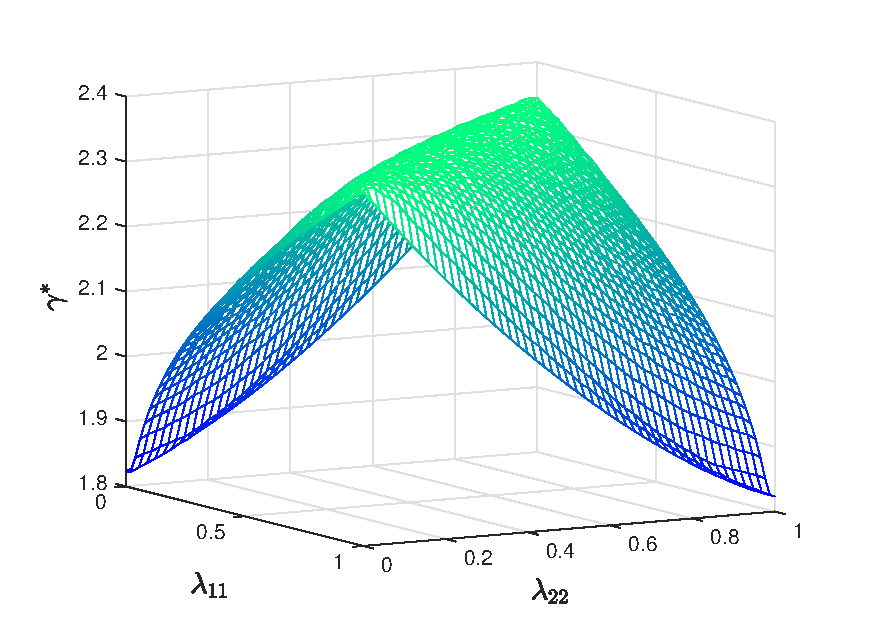
\includegraphics[scale=0.6]{./figures/lure_system/3d3.eps}\\ 
	\caption{最优 $l_2$性能增益 $\gamma^{*}$ 同条件模态转移矩阵 $\varPhi$的关系}
	\label{lure_fig1}
\end{figure}

首先,我们讨论一下最优$\ell_2$性能$\gamma^{*}$同模态转移概率$\varPhi$之间的关系。令
\begin{equation*}
\varPhi=\begin{bmatrix}
\lambda_{11}&1-\lambda_{11} \\
1-\lambda_{22}&\lambda_{22}
\end{bmatrix}
\end{equation*}
其中,$\lambda_{11},\lambda_{22} \in [0,1]$。 图\ref{lure_fig1} 表明最优 $l_2$性能增益 $\gamma^{*}$ 会随着 $\varPhi$的改变而改变。 同时可以观察到下面几个规律

	(1) 在 $\lambda_{11}=\alpha$, $\lambda_{22}=\beta$ 和 $\lambda_{11}=\beta$, $\lambda_{22}=\alpha$ 这两种情况下,$\gamma^{*}$的值是相同的。这个很好理解,毕竟模态的顺序是人为规定的,这两种情况只是将控制器模态定义的顺序改变了一下而已。
	
	(2) 在$\lambda_{11}=0$,$\lambda_{22}=0$ 或 $\lambda_{11}=1$, $\lambda_{22}=1$这两种情况时,最优$\ell_2$性能增益达到最小值 1.8236,实际上,根据我们之前的介绍,在这两种情况下,此时的控制器模态是同系统模态保持一致的,也就是说,这个时候的控制器是一个同步控制器。
	
	(3) 当$\lambda_{11}+\lambda_{22}$的值接近 1 的时候,	$\gamma^{*}$ 的值会变大,这是因为此时控制器的异步率提高了。


下面我们把条件模态转移矩阵中的参数设置为 $\lambda_{11}=0.4$, $\lambda_{22}=0.7$,来进一步研究系统的性能。可以得到如下控制器增益
\begin{equation}\notag
\begin{aligned}
K_{1}=\begin{bmatrix}
-1.4036&-1.3277
\end{bmatrix},\quad
\varGamma_{1}=-2.0473 \\
K_{2}=\begin{bmatrix}
-1.3908&-1.3080
\end{bmatrix},\quad
\varGamma_{2}=-1.8925
\end{aligned}
\end{equation}

\begin{figure}[!htb]
	\centering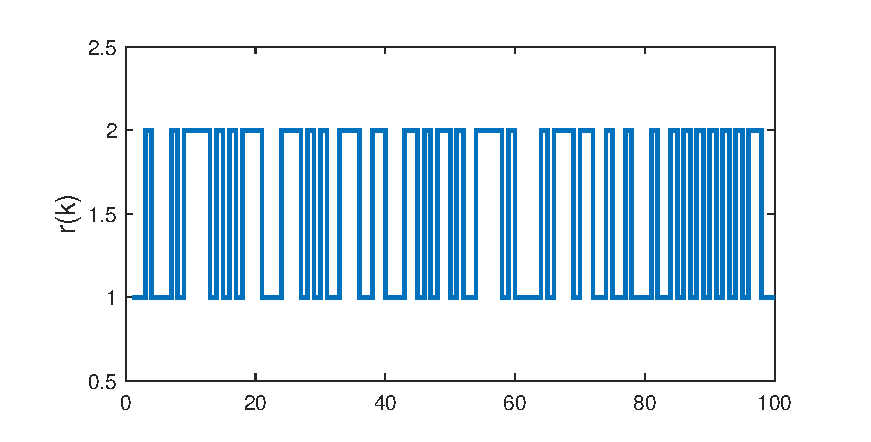
\includegraphics[scale=0.6]{./figures/lure_system/mode_p5.eps}\\ 
	\centering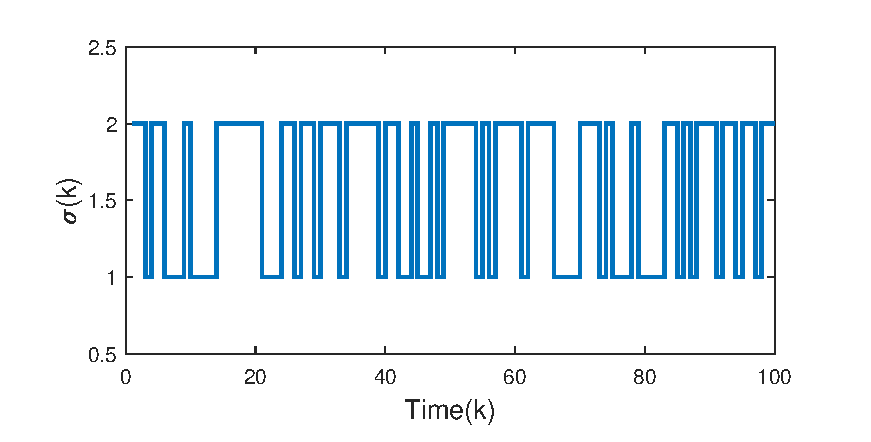
\includegraphics[scale=0.6]{./figures/lure_system/mode_k5.eps}\\ 
	\caption{系统及控制器模态}
	\label{lure_fig2}
\end{figure}

\begin{figure}[!htb]
	\centering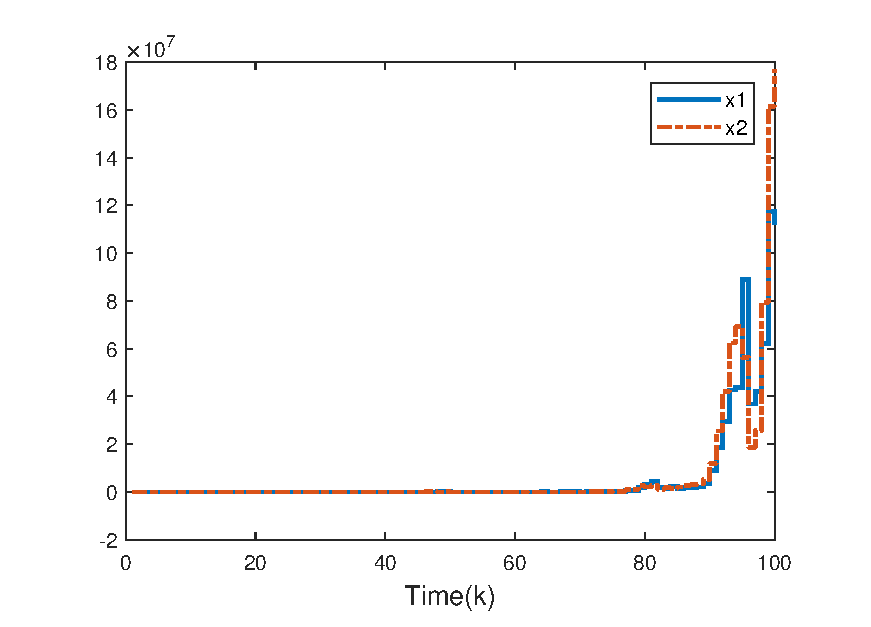
\includegraphics[scale=0.6]{./figures/lure_system/unstable_state2.eps}\\
	\caption{无控制率作用时系统状态变化}
	\label{lure_fig5}
\end{figure}

\begin{figure}[!htb]
	\centering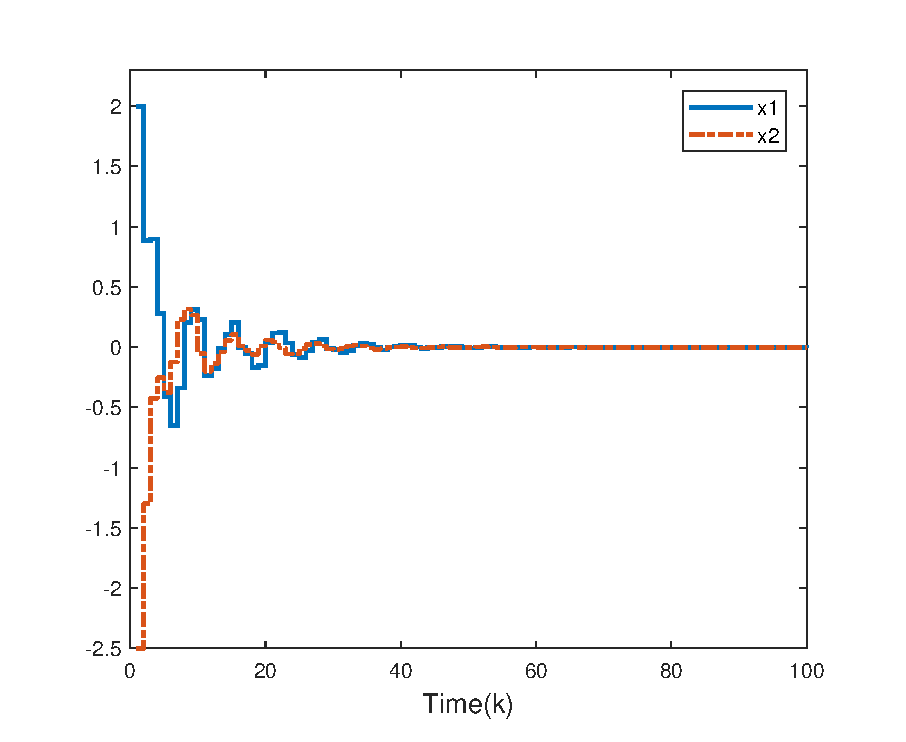
\includegraphics[scale=0.6]{./figures/lure_system/state4.eps}\\
	\caption{有控制率作用时系统状态变化}
	\label{lure_fig3}
\end{figure}
\begin{figure}[!htb]
	\centering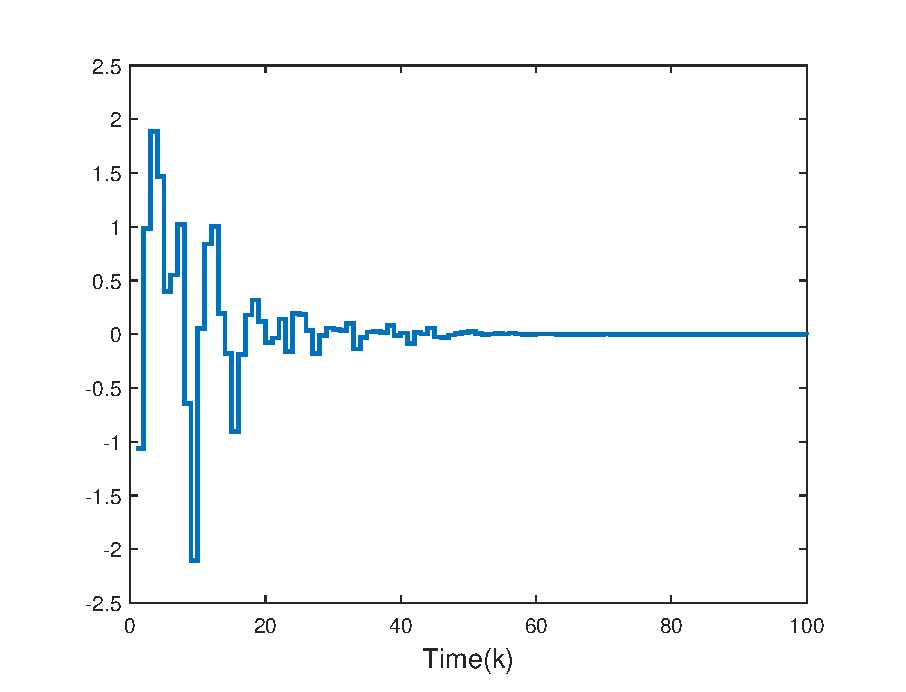
\includegraphics[scale=0.6]{./figures/lure_system/u_k3.eps}\\ 
	\caption{系统输入$u(k)$}
	\label{lure_fig4}
\end{figure}
图\ref{lure_fig2} 给出了一个控制器和系统模态的可能序列。此时,我们选择初始状态为 $x_{0}=\begin{bmatrix}
2&-2.5
\end{bmatrix}^{T}$,外部扰动设置为 $w_{k} = sin(k)*0.85^{k}$。 图\ref{lure_fig5} 表明,当系统在没有施加控制作用的时候是不稳定的。 当我们把控制率施加到系统上时,可以得到系统的状态轨迹如图\ref{lure_fig3}所示。同时,系统的输入$u_{k}$ 如图\ref{lure_fig4} 所示。 由图\ref{lure_fig3}、\ref{lure_fig4}, 我们可以看出,系统状态轨迹在施加我们设计的控制率以后会收敛,表明,此时系统是稳定的。上述实验表明,我们的控制器是异步的,且可以保证系统的稳定性,同时可以保证系统的$\ell_2$性能。


\section{小结}
	本章针对一类特殊的Markov跳变Lur'e系统,我们基于隐Markov模型,设计了一个异步控制器,使得待研究的系统在随机稳定的同时满足了一定的$\ell_2$性能。该异步控制器的特色在于,首先它是个异步控制器,因此比一般的同步控制器、模态独立控制器更加的灵活;其次,它由一个线性状态反馈和一个非线性输出反馈组成,对应了Lue'e系统的结构,这样的结构可以使得得到的结果更加不保守。 然后,根据得到的定理,提出了一个控制器的设计方法,设计的控制器可以使得系统满足随机稳定的同时得到最小的$\ell_2$性能。最后,我们通过了一个数值仿真例子验证了我们设计的控制器的有效性。
% !TEX root = ../thesis.tex

\chapter{模态不匹配2D-Markov跳变系统的异步滑模控制}
	在实际应用中,信息的传递可能会沿着多个维度传递,这样的系统我们称之为多维控制系统。当系统信息的传递方向只有两个的时候,我们称这样的多维系统为二维(2D)控制系统。2D控制系统的历史可以追溯到上个世纪70年代,现在已经被用来处理各种各样的实际应用,例如数字图像处理、偏微分方程建模和信号滤波\cite{roesser1975discrete,marszalek1984two,rogers2015multidimensional}等。同一维(1D)系统不同的是,二维系统的信息会沿着两个不同的方向传递,并且这两个方向的信息会相互作用,这意味着2D系统相对1D系统更加复杂,分析起来也更加困难。 为了描述2D系统的特殊结构和性质,学者们提出了一些基于状态空间的数学模型,其中比较流行的是Roesser模型 \cite{roesser1975discrete} 和 Fornasini-Marchesini 模型 \cite{fornasini1978doubly}。在Roesser模型中,系统状态由水平状态和垂直状态这两个独立的子状态组成,可以从当前状态分别推导出不同方向上的下一个水平状态和垂直状态。 与Roesser模型不同,Fornasini-Marchesini模型中的系统状态并不区分水平、垂直子状态,而是用一个向量来表示两个方向的信息,即该向量是具有两个独立变量的函数,并且当前系统状态是从它的左边相邻、下方相邻状态得到的。 在大多数情况下,Roesser模型可以看作是Fornasini-Marchesini模型的特例,但Rosser模型的表达形式更加直观,更容易理解,在某些情况下更便于系统分析。Du等人在文献\cite{du2001h,du2002hinfinity}中利用2D有界实引理建立了2D系统的$H_\infty$控制理论。随后,一些学者将这个成果推广到了具有时变延迟\cite{trinh2016stability}、多类噪声\cite{ahn2016stochastic}、不确定模态转移参数 \cite{chesi2016robust}等2D系统的控制、滤波问题中。Anh在文献\cite{ahn2015two}中,利用矩阵线性不等式方法研究了2D-Makrov跳变系统的无源控制和滤波问题。
	
	另一方面,滑模控制(SMC)是一种非常有效的控制技术。由于它对参数变化、外部干扰和不确定模型具有强大的鲁棒性,已成功应用于各种实际系统中\cite{utkin2009sliding,yang1999sliding,shima2006sliding}。滑模控制的主要思想是,首先构造一个滑模面,然后根据这个滑模面设计一个不连续的控制率,在该控制率的作用下,系统状态会不断的向滑模面靠近,最终达到滑模面或者进入到滑模面的某个领域内\cite{edwards1998sliding}。近年来,学者们对滑模控制进行了深入的研究,并针对Markov跳变系统取得了一系列重要的成果\cite{li2015state,wu2010state,wang2017smc}。一些学者对1D-Markov跳变系统模态不匹配的滑模控制问题进行了研究\cite{song2018asynchronous,li2017passivity,qi2018observer}。2D-Markov跳变系统同样吸引了一些学者的兴趣。如文献\cite{gao2004stabilization,wu2018hcontrol2d,wu2008hfiltering2d,wu2006modelreduction,shen2019dissipativity}分别对2D-Markov跳变系统的$H_\infty$控制、$H_\infty$滤波、$H_\infty$模型推导、故障检测等问题进行了讨论。但是到目前为止,尚且没有文章研究2D-Markov跳变系统的滑模控制问题。
	
	本章中,我们将研究2D-Markov跳变系统的滑模控制问题。考虑到2D系统的特殊结构和特性,我们将构造一个全新的2D滑模面。另一方面,考虑控制器模态同系统模态的不匹配问题,我们引入隐马尔可夫模型来设计滑模控制器。同时,我们将对系统的稳定性、$H_\infty$性能、系统状态到滑模面的可达性等问题分别展开讨论。

\section{数学模型及问题描述}
	本章考虑如下由Roesser模型描述2D-Markov跳变系统:
	\begin{equation} \label{system-equation}
	\left\{ 
	\begin{array}{lr}
	\begin{split}
	\emph{\textbf{x(i, j)}} = A_{r(i,j)}x(i,j)+B_{r(i,j)}[(u(i,j)+f(x(i,j),r(i,j))]+E_{r(i,j)}w(i,j),
	\end{split}\\
	\begin{split}
	y(i,j) = C_{r(i,j)}x(i,j)+D_{r(i,j)}w(i,j),
	\end{split}
	\end{array}
	\right.
	\end{equation}
	其中,
	\begin{equation*}
	\emph{\textbf{x(i, j)}} = \begin{bmatrix}
	x^{h}(i+1,j)\\
	x^{v}(i,j+1)
	\end{bmatrix}, \ 
	x(i, j) = \begin{bmatrix}
	x^{h}(i,j)\\
	x^{v}(i,j)
	\end{bmatrix}          
	\end{equation*}
	这里,	$x^{h}(i,j)\in \mathbb{R}^{n_h}$, $x^{v}(i,j)\in \mathbb{R}^{n_v}$ 分别表示水平、垂直两个方向的子系统状态, $u(i,j) \in \mathbb{R}^{n_u}$,$y(i,j) \in \mathbb{R}^{n_y}$ 分别表示控制输入和被控输出, 以及 $w(i,j) \in \mathbb{R}^{n_w}$ 表示外部扰动,并满足条件$\ell_{2}\{[0,\infty),[0,\infty)\}$。 $A_{r(i,j)}$, $B_{r(i,j)}$, $C_{r(i,j)}$, $D_{r(i,j)}$ 及 $E_{r(i,j)}$ 表示已知具有合适维度的系统时变矩阵。 同时,我们假设对任意的 $r(i,j)\in\mathcal{N}_{1}$,矩阵$B_{r(i,j)}$是列满秩的,即rank($B_{r(i,j)}$)$=n_u$。 非线性函数 $f(x(i,j),r(i,j))$ 满足
	\begin{equation}\label{nonlinear-func}
	\|f(x(i,j),r(i,j)\| \leq \delta_{r(i,j)}\|x(i,j)\|
	\end{equation}
	其中, $\delta_{r(i,j)}$ 是一个已知的标量, $\|\cdot\|$ 表示欧拉范数。 参数 $r(i,j)$ 在集合 $\mathcal{N}_{1}=\{1,2...,N_{1} \}$ 中取值,同时满足模态转移矩阵 $\varLambda = [\lambda_{kp}]$,其对应的模态转移概率为  (参考文献\cite{wu2018hcontrol2d,wu2008hfiltering2d})
	\begin{equation}\label{tps_system}
	\begin{split}
	&\Pr\{r(i+1,j)=p|r(i,j)=k\}\\
	=&\Pr\{r(i,j+1)=p|r(i,j)=k\}=\lambda_{kp},\  \forall k,p \in \mathcal{N}_{1}
	\end{split}
	\end{equation}	
	这里,对任意的  $k, p\in\mathcal{N}_{1}$, $\lambda_{kp}\in[0,1]$,且对任意的 $k$,有$\sum_{p=1}^{N_1}\lambda_{kp}=1$。
	
	{\bf 注 \ \ 3.1:}
	注意到,条件\eqref{tps_system} 包含了一个隐含的假设,即系统模态沿着水平、垂直方向的跳变概率是一样的。
	
	下面我们对2D系统\eqref{system-equation}的初始条件 ($X_{0},\varGamma_{0}$) 做以下假设
	\begin{equation} \label{boundary-condition}
	\left\{
	\begin{array}{lr}
	\begin{split}
	X_{0} &= \{x^{h}(0,j),x^{v}(i,0)|\ i,j = 0,1,2...\}\\
	\varGamma_{0} &= \{r(0,j), r(i,0)|\ i,j = 0,1,2... \}
	\end{split}
	\end{array}
	\right.
	\end{equation}
	
	系统状态的零初始条件$X_0$设置为,对任意非负整数$i,j$,$x^{h}(0,j) =0, x^{v}(i,0)=0$。此外,对$X_{0}$施加如下假设
	
	{\bf 假设 \ \ 3.1:}
	边界条件$X_{0}$满足
	\begin{equation}
	\lim\limits_{Z\to\infty}\mathbb{E}\Big\{\sum_{z=1}^{Z}(\|x^{h}(0,z)\|^{2}+ \|x^{v}(z,0)\|^{2})\Big\} < \infty
	\end{equation}
	其中,$\mathbb{E}\{\cdot\}$表示数学期望。
	
	在实际控制系统中,控制器往往不能获得系统模态$r(i,j)$的全部信息。因此,在本章中,我们采用了隐Markov模型$(r(i,j),\sigma(i,j),\varLambda,\varPsi)$来描述控制器模态和系统模态之间存在的不匹配现象。这里,我们使用$\sigma(i,j)$来表示控制器模态,它在另一个集合$\mathcal{N}_{2} = \{1,2...N_{2}\}$中取值,且满足条件模态转移矩阵$\varPsi=[\mu_{k\tau} ]$,该矩阵对应的条件模态转移概率为
	\begin{equation}
	\Pr\{\sigma(i,j)=\tau|r(i,j)=k\}=\mu_{k\tau } %\forall  k\in\mathcal{N}_{1}, \tau\in\mathcal{N}_{2}
	\end{equation}
	这里,对任意的$k\in\mathcal{N}_{1}$,$\tau\in\mathcal{N}_{2}$, 有$\mu_{k\tau }\in[0,1]$,且对任意的模态$k$,有 $\sum_{\tau =1}^{N_{2}}\mu_{k\tau } = 1$ 。
	
	{\bf 注 \ \ 3.2:}
	隐Markov模型是一个包含了同步、异步及模态独立情况的综合模型。控制器属于哪种情况可由条件模态转移概率矩阵$\varPsi$来决定。当$\varPsi=\varLambda$时,控制器变成了一个模态同步控制器,当$\mathcal{N}_{2}=\{1\}$时,控制器变成了一个只包含一个模态的模态独立控制器。因此,我们得到的结果可以通过调节矩阵$\varPsi$,很容易推广到同步和模态独立的情况。
	
	下面,我们分别给出系统渐进均方稳定和 $H_{\infty}$ 性能的定义。	
	
	{\bf 定义 \ \ 3.1:}
	当$w(i,j)\equiv0$时, 如果下式对任意的初始条件$X_{0}$成立
	\begin{equation}\label{AMSS}
	\lim\limits_{i+j\to\infty}\mathbb{E}\{\|x(i,j)\|^{2}\} = 0
	\end{equation}
	我们称,在假设3.1意义下的2D-Markov跳变系统 \eqref{system-equation}是渐进均方稳定的。
	
	{\bf 定义 \ \ 3.2:}
	给定标量 $\gamma>0$,如果条件 \eqref{AMSS}及下面的公式在$w(i,j)\in\ell_{2}\{[0,\infty),[0,\infty)\}$时成立,
	\begin{equation} \label{invDef2}
	\sum_{i=0}^{\infty}\sum_{j=0}^{\infty}\mathbb\{\|y(i,j)\|^{2}\} <  \gamma^{2} \sum_{i=0}^{\infty}\sum_{j=0}^{\infty}\mathbb\{\|w(i,j)\|^{2}\}
	\end{equation}
	我们称,在零初始条件下的2D-Markov跳变系统\eqref{system-equation}是渐进均方稳定的,同时满足$H_{\infty}$性能$\gamma$。

	为了方便后续的推导,我们这里做一些符号简化。我们使用$k$来表示参数$r(i,j)$,使用$\tau$来表示$\sigma(i,j)$ 。

	本章的目的是,基于隐Markov模型,设计一个二维异步控制器,使得对应的Markov跳变系统是随机稳定的,并满足一定的$H_{\infty}$性能。
	
\section{主要成果}
	在本节,我们首先根据2D系统的结构特征,构造一个新颖的2D滑模面,同时基于隐Markov模型设计出对应的2D滑模控制器。之后,我们会分析系统的渐进均方稳定性,$H_{\infty}$性能,以及系统状态到滑模面的可达性。

\subsection{滑模面构造及异步2D滑模控制器设计} \label{sliding-surface}
	在本章中,我们根据2D系统的特性构造如下滑模面
	\begin{equation}\label{siding-surface-equation}	
	s(i,j) = \begin{bmatrix}
	s^{h}(i,j)\\
	s^{v}(i,j)
	\end{bmatrix}
	= Gx(i,j)
	\end{equation}
	这里,$s^{h}(i,j)$、 $s^{v}(i,j)$分别代表水平、垂直方向的子滑模面,矩阵$G=\sum_{k=1}^{N_{1}}\beta_{k}B^{T}_{k}$。 这里需要注意的是,我们应该选择合适的 $\beta_{k}$ 使得矩阵$GB_{k}$ 对任意的$k\in\mathcal{N}_{1}$都是非齐次的。 根据假设 $B_{k}$ 对任意的$k\in\mathcal{N}_{1}$是列满秩的, 因此只要选择合适的 $\beta_{k}$就一定可以使得上述要求得以满足。 
	
	考虑到控制器模态同系统模态的不匹配问题,设计如下的异步2D滑模控制器
	\begin{equation}\label{smc-law}
	u(i,j) = K_{\tau }x(i,j)-\rho(i,j)\frac{s(i,j)}{\|s(i,j)\|}
	\end{equation}
	这里,矩阵$K_{\tau }\in\mathbb{R}^{n_u\times n_x}$是待确定的控制器增益, 且满足 $n_x=n_h+n_v$, 参数 $\rho(i,j)$ 设定为
	\begin{equation}\label{varrho}
	\rho(i,j) = \varrho_{1}\|x(i,j)\| + \varrho_{2}\|w(i,j)\|
	\end{equation}
	其中, $\varrho_{1}=\max_{k\in\mathcal{N}_{1}} \{\delta_{k} \}$, $\varrho_{2} = \max_{k\in\mathcal{N}_{1}}\{\|(GB_{k})^{-1}GE_{k}\| \} $, 参数 $\delta_{k}$ 在条件\eqref{nonlinear-func}中已经给出。 
	
	由系统方程\eqref{system-equation}及异步2D控制器\eqref{smc-law},我们可以得到如下闭环2D-Markov跳变系统
	\begin{equation} \label{closed-loop-system-equation}
	\emph{\textbf{x(i, j)}} = \bar{A}_{k\tau }x(i,j)+B_{k}\bar{\rho}_{k}(i,j)+E_{k}w(i,j)
	\end{equation}
	其中, $\bar{A}_{k\tau } = A_{k}+B_{k}K_{\tau }$,$\bar{\rho}_{k}(i,j)$ 为
	\begin{equation*}
	\bar\rho_{k}(i,j)=f_{k}(x(i,j))-\big(\varrho_{1}\|x(i,j)\|+\varrho_{2}\|w(i,j)\|\big)\cdot\frac{s(i,j)}{\|s(i,j)\|}.
	\end{equation*}
	下面,根据 \eqref{nonlinear-func} 及向量范数的性质, 我们可以推出
	\begin{equation}\label{norm-rho-inequality}
	\|\bar{\rho}_{k}(i,j)\| \leq (\varrho_{1}+\delta_{k})\|x(i,j)\| + \varrho_{2}\|w(i,j)\| ,
	\end{equation} 
	进一步可以得到
	\begin{equation}\label{rholeseq}
	\|\bar{\rho}_{k}(i,j)\|^{2} \leq 2(\varrho_{1}+\delta_{k})^{2}\|x(i,j)\|^{2} +2\varrho_{2}^{2}\|w(i,j\|^{2} .
	\end{equation}	
	
	{\bf 注 \ \ 3.3:}
	本文设计的控制器基于隐Markov模型 $(r(i,j),\sigma(i,j),\varLambda,\varPsi)$,在这个模型下,系统的模态由Markov过程$\{r(i,j), i,j=1,2\ \dots\}$控制,而控制器的模态则由条件转移概率$u_{k\tau}$得到,条件模态转移概率矩阵$\varPsi$建立了系统模态和控制器模态之间的联系,相比模态独立控制器更充分的利用了系统的模态信息,这是异步控制器相比模态独立控制器的一个优势。
	
	{\bf 注 \ \ 3.4:}
	正如在前文中所介绍的,1D滑模控问题已经获得了广泛的研究,比如文献\cite{song2018asynchronous,li2017passivity,qi2018observer}等。但是值得注意的是,2D滑模控制(不仅仅是异步控制)问题目前还没有人进行研究。实际上,2D系统的特殊性质给系统分析带来了更大的复杂性,1D系统得到的诸多结论不能直接的推广到2D系统中来,2D系统的滑模控制问题相对1D系统更加的复杂。因此我们需要从2D系统的结构出发,来研究2D系统的滑模控制问题。在本章中,我们基于Roesser模型的2D系统特性,重新的设计了一个二维滑模面$s(i,j)$,由于2D滑模控制率包含了 $x(i,j)$ 、$s(i,j)$,因此我们称所设计的滑模控制器是2D滑模控制器。

\subsection{稳定性及 $H_{\infty}$ 性能分析 } \label{stability&H_infty}	
	在本小节,我们将关注闭环2D-Markov跳变系统\eqref{closed-loop-system-equation}的稳定性及$H_{\infty}$ 性能分析。我们将会提出一个充分条件,使得系统渐进均方稳定,且满足一个$H_{\infty}$ 性能 $\gamma$。
	
	{\bf 定理 \ \ 3.1:}
	考虑满足假设3.1,在2D异步滑模控制率\eqref{smc-law}作用下的2D控制系统\eqref{system-equation}。 对任意的$k\in\mathcal{N}_{1}, \tau\in\mathcal{N}_{2}$,给定标量 $\gamma>0$,如果存在矩阵 $K_{\tau }\in\mathbb{R}^{n_u\times n_x}$,  $R_{k}=\mathrm{diag}\{R^{h}_{k},R^{v}_{k}\}>0$,  $Q_{k\tau }>0$, $T_{k\tau }>0$ ,标量$\epsilon_{k}>0$, 有下列不等式成立
	\begin{equation}\label{T1C1}
	B^{T}_{k}  	\mathcal{R}_{k} B_{k} -\epsilon_{k}I \leq 0
	\end{equation}
	\begin{equation}\label{T1C2}
	\mathcal{A} +2\Big(\sum_{\tau =1}^{N_{2}}\mu_{k\tau } \mathrm{diag}\{Q_{k\tau }, T_{k\tau }\}\Big) < 0
	\end{equation}
	\begin{equation}\label{T1C3}
	\hat{A}^{T}_{k\tau }\mathcal{R}_{k}\hat{A}_{k\tau } - \mathrm{diag}\{Q_{k\tau }, T_{k\tau }\} < 0
	\end{equation}
	其中,
	\begin{equation*}
	\mathcal{A}=\begin{bmatrix}
	\varPi_{1} & \varPi_{3}\\
	*&\varPi_{2}
	\end{bmatrix}
	\end{equation*} 且,
	\begin{equation*} \label{varPi}
	\left\{
	\begin{array}{lr}
	\begin{split}
	\varPi_{1}&=-R_{k}+4(\delta_{k}+\varrho_{1})^{2}\epsilon_{k}I+C^{T}_{k}C_{k}\\
	\varPi_{2}&=-\gamma^{2}I+D^{T}_{k}D_{k}+4\varrho_{2}^{2}\epsilon_{k}I\\
	\varPi_{3}&= C_{k}^{T}D_{k}\\
	\end{split}
	\end{array}
	\right.
	\end{equation*}
	这里,$\mathcal{R}_{k}=\sum_{p=1}^{N1}\lambda_{kp}R_{p}$, $\hat{A}_{k\tau }=\begin{bmatrix}
	\bar{A}_{k\tau }& E_{k}
	\end{bmatrix}$。
	那么,我们称闭环2D-Markov跳变系统\eqref{closed-loop-system-equation} 是渐进均方稳定的,且满足 $H_{\infty}$性能$\gamma$。
	
	{\bf 证明:} 
	我们首先来研究系统的稳定性问题。 选择李雅普诺夫函数为 $V_{1}(i,j) = x^{T}(i,j)R_{r(i,j)}x(i,j)$,并定义
	\begin{equation}\label{VAR-DELTA-V1}
	\begin{split}
	\varDelta V_{1}(i,j) = \emph{\textbf{x(i, j)}}^{T} R^{*}(i,j) \emph{\textbf{x(i, j)}} - x^{T}(i,j)R_{k}x(i,j)
	\end{split}
	\end{equation}
	这里,$R^{*}(i,j)=\mathrm{diag}\{R^{h}_{r(i+1,j)},R^{v}_{r(i,j+1)}\}$。\\
	在$w(i,j)=0$时,由闭环控制系统 \eqref{closed-loop-system-equation},我们可以得到 
	\begin{equation}
	\begin{split}
	\mathbb{E}\{\varDelta V_{1}(i,j) \}&=\mathbb{E}\{\emph{\textbf{x(i, j)}}^{T}\mathcal{R}_{k}\emph{\textbf{x(i, j)}} - x^{T}(i,j)R_{k}x(i,j) \} \\
	&=  \sum_{\tau =0}^{N_{2}}\mu_{k\tau }\Big\{\big[\bar{A}_{k\tau }x(i,j)+B_{k}\bar{\rho}_{k}(i,j)\big]^{T}\mathcal{R}_{k}\\
	&\times\big[\bar{A}_{k\tau }x(i,j)+B_{k}\bar{\rho}_{k}(i,j)\big]\Big\}\\
	&- x^{T}(i,j)R_{k}x(i,j) \\
	&\leq x^{T}(i,j) \Big\{2\big(\sum_{\tau =1}^{N_{2}}\mu_{k\tau }\bar{A}^{T}_{k\tau }(i,j)\mathcal{R}_{k}\bar{A}_{k\tau }\big)\Big\}x(i,j)\\ &+2\bar{\rho}^{T}_{k}(i,j)B^{T}_{k}\mathcal{R}_{k}B_{k}\bar{\rho}_{k}(i,j) \\
	&-  x^{T}(i,j)R_{k}x(i,j)
	\end{split}
	\end{equation}
	由条件\eqref{norm-rho-inequality} 、\eqref{T1C1},可以推出
	\begin{equation}\label{combine-one-1}
	\begin{split}
	\mathbb{E}\{\varDelta  V_{1}(i,j) \} \leq x^{T}(i,j)\mathcal{G}_{k\tau }x(i,j)
	\end{split}
	\end{equation}
	其中, $\mathcal{G}_{k\tau }= 2\big(\sum_{\tau =1}^{N_{2}}\mu_{k\tau }\bar{A}^{T}_{k\tau }\mathcal{R}_{k}\bar{A}_{k\tau }\big)
	+ 2\epsilon_{k}(\delta_{k}+\varrho_{1})^{2}I- R_{k}$。
	根据正定矩阵的性质,可以由 \eqref{T1C2} ) 推出
	\begin{equation}
	2\big(\sum_{\tau =1}^{N_{2}}\mu_{k\tau }Q_{k\tau }\big)+4\epsilon_{k}(\delta_{k}+\varrho_{1})^{2}I+C^{T}_{k}C_{k}-R_{k} < 0
	\end{equation}
	进一步可以得到
	\begin{equation}\label{combine-one-2}
	2\big(\sum_{\tau =1}^{N_{2}}\mu_{k\tau }Q_{k\tau }\big)+2\epsilon_{k}(\delta_{k}+\varrho_{1})^{2}I-R_{k} < 0
	\end{equation}
	由条件 \eqref{T1C3}可以得到 
	\begin{equation}\label{combine-one-3}
	\bar{A}^{T}_{k\tau }\mathcal{R}_{k}\bar{A}_{k\tau }-Q_{k\tau } < 0
	\end{equation}
	由\eqref{combine-one-2}、\eqref{combine-one-3} 可以发现 $\mathcal{G}_{k\tau }<0$, 等价于
	\begin{equation}
	\mathcal{G}_{k\tau } \leq -\alpha I
	\end{equation}
	这里 $\alpha>0$。
	根据 \eqref{combine-one-1} 我们可以进一步得到
	\begin{equation}\label{VleqAlpha}
	\mathbb{E}\{\varDelta V_{1}(i,j) \} \leq-\alpha \mathbb{E}\{\|x(i,j)\|^{2} \}
	\end{equation}
	对上式累加\eqref{VleqAlpha}推出
	\begin{equation} \label{levE}
	\mathbb{E}\Big\{\sum_{i=0}^{\hat{\kappa}_{1}}\sum_{j=0}^{\hat{\kappa}_{2}}  \|x(i,j)\|^{2} \Big\} \leq -\frac{1}{\alpha} \mathbb{E}\Big\{\sum_{i=0}^{\hat{\kappa}_{1}}\sum_{j=0}^{\hat{\kappa}_{2}}  \varDelta V_{1}(i,j)  \Big\}
	\end{equation}
	这里 $\hat{\kappa}_{1}$, $\hat{\kappa}_{2}$ 是任意的正整数。 用 \eqref{VAR-DELTA-V1} 来代替 $\varDelta V_{1}$,同时,令 $R_{k}=\mathrm{diag}\{R^{\rm{h}}_{k},R^{\rm{v}}_{k}\}$ (见定理3.1) ,可以推出
	\begin{equation} \label{Vhv}
	\begin{split}
	&\sum_{i=0}^{\hat{\kappa}_{1}}\sum_{j=0}^{\hat{\kappa}_{2}}  \varDelta V_{1}(i,j)\\&= \sum_{i=0}^{\hat{\kappa}_{1}}\big\{V^{v}_{1}(i,\hat{\kappa}_{2}+1) - V^{v}_{1}(i,0) \big\}+  \sum_{j=0}^{\hat{\kappa}_{2}}\big\{V^{h}_{1}(\hat{\kappa}_{1}+1,j) - V^{h}_{1}(0,j) \big\}\\
	&\leq -\big( \sum_{i=0}^{\hat{\kappa}_{1}}V^{v}_{1}(i,0) + \sum_{j=0}^{\hat{\kappa}_{2}}V^{h}_{1}(0,j)\big) \\
	%			&\leq -\beta \sum_{\ell=0}^{\infty} \big(  \|x^{v}(\ell,0)\|^{2} + \|x^{h}(0,\ell)\|^{2} \big)
	\end{split}
	\end{equation} 
	这里,我们定义$V_{1}^{h}(i,j)$ 和 $V_{1}^{v}(i,j)$ 如下  
	\begin{equation*}
	\left\{
	\begin{array}{lr}
	\begin{split}
	V^{h}_{1}(i,j)=x^{hT}(i,j)R^{h}_{r(i,j)}x^{h}(i,j)\\
	V^{v}_{1}(i,j)=x^{vT}(i,j)R^{v}_{r(i,j)}x^{v}(i,j)
	\end{split}
	\end{array}
	\right.
	\end{equation*}
	根据边界条件假设3.1,同时令$\hat{\kappa}_{1}$, $\hat{\kappa}_{2}$ 趋向无穷, 由\eqref{levE} 及\eqref{Vhv} 可以推出
	\begin{equation}
	\begin{split}
	\mathbb{E}\Big\{\sum_{i=0}^{\hat{\kappa}_{1}}\sum_{j=0}^{\hat{\kappa}_{2}}  \|x(i,j)\|^{2} \Big\} &\leq \frac{\beta}{\alpha} \sum_{\ell=0}^{\infty} \big(  \|x^{v}(\ell,0)\|^{2} + \|x^{h}(0,\ell)\|^{2} \big)<\infty
	\end{split}	
	\end{equation}
	这里 $\beta$ (显然,$\beta>0$) 是对任意的$\ell=0,1,2...$,$R^{h}_{r(0,\ell)}$ 和 $R^{v}_{r(\ell,0)}$的最大特征值。上式意味着 \eqref{AMSS} 成立。至此,我们证明了闭环控制系统是渐进均方稳定的。
	
	下面我们来研究在零初始条件下系统的$H_{\infty}$性能问题。 根据闭环控制系统\eqref{closed-loop-system-equation},不难推出
	\begin{equation}\label{DETAV1}
	\begin{split}
	\mathbb{E}\{\varDelta V_{1}(i,j) \} &=  \sum_{\tau =0}^{N_{2}}\mu_{k\tau }\Big\{\big[\bar{A}_{k\tau }x(i,j)+B_{k}\bar{\rho}_{k}(i,j)+E_{k}w(i,j)\big]^{T}\\
	&\times \mathcal{R}_{k}\big[\bar{A}_{k\tau }x(i,j)+B_{k}\bar{\rho}_{k}(i,j)+E_{k}w(i,j)\big]\Big\}\\
	&- x^{T}(i,j)R_{k}x(i,j) \\
	&\leq \hat{x}^{T}(i,j) \Big\{2\big(\sum_{\tau =1}^{N_{2}}\mu_{k\tau }\hat{A}^{T}_{k\tau }(i,j)\mathcal{R}_{k}\hat{A}_{k\tau }\big)\Big\}\hat{x}(i,j)\\ &+2\bar{\rho}^{T}_{k}(i,j)B^{T}_{k}\mathcal{R}_{k}B_{k}\bar{\rho}_{k}(i,j) \\
	&-  x^{T}(i,j)R_{k}x(i,j)\\
	\end{split}
	\end{equation}
	%	where $\hat{x}(i,j)=\begin{bmatrix}
	%		x(i,j)\\ w(i,j)
	%	\end{bmatrix}$, $\hat{A}_{k\tau }(i,j)=\begin{bmatrix}
	%		\bar{A}_{k\tau }&E_{k}
	%	\end{bmatrix}$.
	这里
	\begin{equation*}
	\hat{x}(i,j)=\begin{bmatrix}
	x(i,j)\\ w(i,j)
	\end{bmatrix},\ \hat{A}_{k\tau }(i,j)=\begin{bmatrix}
	\bar{A}_{k\tau }&E_{k}
	\end{bmatrix}
	\end{equation*}
	注意到条件 \eqref{rholeseq} 及\eqref{T1C1},可以推出
	\begin{equation}\label{invRho}
	\begin{split}
	&\bar{\rho}^{T}_{k}(i,j)B^{T}_{k}\mathcal{R}_{k}B_{k}\bar{\rho}_{k}(i,j)\\
	&\leq \|B^{T}_{k}\mathcal{R}_{k}B_{k}\|\|\bar{\rho}_{k}\|^{2} \\
	&\leq 2\epsilon_{k}\big((\delta_{k}+\varrho_{1})^{2}\|x(i,j)\|^{2}+\varrho_{2}^{2}\|w(i,j)\|^{2} \big)
	\end{split}
	\end{equation} 
	由条件 \eqref{T1C2} 及 \eqref{T1C3}可以得到下式
	\begin{equation}\label{T1P4}
	\mathcal{\varXi}_{k\tau }<0
	\end{equation}	
	其中, $\mathcal{\varXi}_{k\tau } \equiv \mathcal{A} +2\sum_{\tau =1}^{N_{2}}\mu_{k\tau }\hat{A}^{T}_{k\tau }\mathcal{R}_{k}\hat{A}_{k\tau }$。
	由系统方程 \eqref{system-equation},且把\eqref{invRho} 带入 \eqref{DETAV1} 可以得到
	\begin{equation}\label{DETAV1ZW}
	\begin{split}
	\mathbb{E}\{\varDelta V_{1}(i,j)+\|y(i,j)\|^{2}-\gamma^{2}\|w(i,j)\|^{2}  \} \leq \hat{x}^{T}(i,j)\mathcal{\varXi}_{k\tau } \hat{x}(i,j)<0
	\end{split}
	\end{equation}
	注意到在零初始条件下的\eqref{Vhv} 我们可以推出
	\begin{equation} \label{Vhv2}
	\begin{split}
	&\sum_{i=0}^{\hat{\kappa}_{1}}\sum_{j=0}^{\hat{\kappa}_{2}}  \varDelta V_{1}(i,j)\\
	&=\sum_{i=0}^{\hat{\kappa_{1}}}V^{v}_{1}(i,\hat{\kappa}_{2}+1) + \sum_{j=0}^{\hat{\kappa}_{2}}V^{h}_{1}(\hat{\kappa}_{1}+1,j) \\
	&\geq 0 \qquad \forall \hat{\kappa}_{1},\hat{\kappa}_{2} = 1,2,3...
	\end{split}
	\end{equation}
	接下来,由 \eqref{DETAV1ZW} 和 \eqref{Vhv2} 我们可以得到 
	\begin{equation}\label{DETAV1ZW2}
	\begin{split}
	&\sum_{i=0}^{\infty}\sum_{j=0}^{\infty}  \mathbb{E}\{\|y(i,j)\|^{2}-\gamma^{2}\|w(i,j)\|^{2}  \}\\
	&\leq \sum_{i=0}^{\infty}\sum_{j=0}^{\infty}  \mathbb{E}\{\varDelta V_{1}(i,j)+\|y(i,j)\|^{2}-\gamma^{2}\|w(i,j)\|^{2}  \}  \\
	&< 0
	\end{split}
	\end{equation}
	进而 \eqref{invDef2}成立。 至此,我们完成了定理的证明。
	
\subsection{滑模面可达性分析}\label{minimization} 
	在本小节,我们将会分析在设计的异步控制率作用下的系统状态到所构造滑模面的可达性问题。借助Lyapunov方法,我们会提供一个充分条件,使得在异步滑模控制率\eqref{smc-law}可以迫使系统状态轨迹进入到一个预先设定的滑模域内部。
	
	{\bf 定理 \ \ 3.2:}
	考虑在异步2D滑模控制率作用下的闭环2D-Markov跳变系统\eqref{closed-loop-system-equation}。如果对任意的$k\in\mathcal{N}_{1}$,$\tau\in\mathcal{N}_{2}$,存在矩阵 $K_{\tau }\in\mathbb{R}^{n_u\times n_x}$, $R_{k}>0$, $F_{k}>0$,标量 $\epsilon_{k}>0$,  使得条件 \eqref{T1C1} 及下面的式子成立
	\begin{equation} \label{T2C1}
	2\sum_{\tau =1}^{N_{2}} \bar{A}^{T}_{k\tau }\big(\mathcal{R}_{k}+G^{T}\mathcal{F}_{k}G\big)\bar{A}_{k\tau }-R_{k} <0
	\end{equation}
	这里, $\mathcal{R}_{k}$ 在定理 3.1中定义了,且矩阵 $\mathcal{F}_{k}=\sum_{p=1}^{N_{1}}\lambda_{kp}F_{p}$。那么,闭环2D控制系统   \eqref{closed-loop-system-equation} 的系统状态将会进入一个滑模域 $\mathcal{O}$内,该滑模域围绕预先定义的滑模面 \eqref{siding-surface-equation},且定义为
	\begin{equation}\label{smc-region}
	\mathcal{O}\equiv\Big\{\|s(i,j)\|\leq\ \rho^{*}(i,j) \Big\}
	\end{equation} 
	这里$\rho^{*}(i,j) = \mathrm{max}_{k\in\mathcal{N}_{1}}\sqrt{\hat{\rho}_{k}(i,j)/
		\lambda_{\mathrm{min}}(F_{k})}$,其中
	\begin{equation*}
	\begin{split}
	\hat{\rho}_{k}(i,j)=&4\big(\|E^{T}_{k}\mathcal{R}_{k}E_{k}\|+ \|E^{T}_{k}G^{T}\mathcal{R}_{k}GE_{k}\|\\
	&+2\varrho_{2}^{2}(\|B^{T}_{k}\mathcal{F}_{k}B_{k}\|+ \|B^{T}_{k}G^{T}\mathcal{F}_{k}GB_{k}\| )\big)\|w(i,j)\|^{2}\\
	+&8(\varrho_{1}+\delta_{k})^{2}\big(\|B^{T}_{k}\mathcal{R}_{k}B_{k}\|+\|B^{T}_{k}G^{T}\mathcal{R}_{k}GB_{k}\|\big)\|x(i,j)\|^{2}.
	\end{split}
	\end{equation*}
	这里 $\lambda_{\mathrm{min}}(F_{k})$ 在此时表示矩阵 $F_{k}$的最小特征值。
	
	{\bf 证明:} 
	首先,我们定义$\emph{\textbf{s(i, j)}} = \begin{bmatrix}
	s^{h}(i+1,j)\\ s^{v}(i,j+1)
	\end{bmatrix}$,  显然$\emph{\textbf{s(i, j)}}=G\emph{\textbf{x(i, j)}}$。 然后我们选择如下李雅普诺夫函数
	\begin{equation}\label{LyapunoovT}
	V(i,j)=V_{1}(i,j)+V_{2}(i,j)
	\end{equation}
	这里 $V_{1}(i,j)$ 同定理3.1, $V_{2}(i,j)=s^{T}(i,j)F_{r(i,j)}s(i,j)$。 同定理3.1的证明过程相似,我们不难推出
	\begin{equation} \label{P2T1}
	\begin{split}
	&\mathbb{E}\{\varDelta V_{1}(i,j) \}\\
	&=\mathbb{E}\Big\{\emph{\textbf{x(i, j)}}^{T}R^{*}(i,j)\emph{\textbf{x(i, j)}} - x^{T}(i,j)R_{k}x(i,j)\Big\}\\
	&=  \sum_{\tau =0}^{N_{2}}\mu_{k\tau }\Big\{\big[\bar{A}_{k\tau }x(i,j)+B_{k}\bar{\rho}_{k}(i,j)+E_{k}w(i,j)\big]^{T}\\
	&\times\mathcal{R}_{k} \big[ \bar{A}_{k\tau }x(i,j)+B_{k}\bar{\rho}_{k}(i,j)+E_{k}w(i,j)\big]\Big\}\\
	&-x^{T}(i,j)R_{k}x(i,j)\\
	&\leq 2x^{T}(i,j)\sum_{\tau =1}^{N_{2}}\mu_{k\tau }\bar{A}^{T}_{k\tau }\mathcal{R}_{k}\bar{A}_{k\tau }x(i,j) \\
	&+2\big[B_{k}\bar{\rho}_{k}(i,j)+E_{k}w(i,j)\big]^{T}\mathcal{R}_{k} \big[B_{k}\bar{\rho}_{k}(i,j)+E_{k}w(i,j)\big]
	-x^{T}(i,j)R_{k}x(i,j)\\
	&\leq 2x^{T}(i,j)\sum_{\tau =1}^{N_{2}}\mu_{k\tau }\bar{A}^{T}_{k\tau }\mathcal{R}_{k}\bar{A}_{k\tau }x(i,j) 
	+ 4\bar{\rho}^{T}_{k}(i,j)B^{T}_{k}\mathcal{R}_{k}B_{k}\bar{\rho}_{k}(i,j)\\
	&+4w^{T}(i,j)E^{T}_{k}\mathcal{R}_{k}E_{k}w(i,j)
	-x^{T}(i,j)R_{k}x(i,j)
	%&\mathbb{E}\{\varDelta V_{1}(i,j) \}\\
	%=&\mathbb{E}\Big\{\emph{\textbf{x(i, j)}}^{T}R_{p}\emph{\textbf{x(i, j)}} - x^{T}(i,j)R_{k}x(i,j)\Big\}\\
	%=&  \sum_{\tau =0}^{N_{2}}\mu_{k\tau }\Big\{\big[\bar{A}_{k\tau }x(i,j)+B_{k}\bar{\rho}_{k}(i,j)+E_{k}w(i,j)\big]^{T}\\
	%\times&\mathcal{R}_{k} \big[ \bar{A}_{k\tau }x(i,j)+B_{k}\bar{\rho}_{k}(i,j)+E_{k}w(i,j)\big]\Big\}\\
	%-&x^{T}(i,j)R_{k}x(i,j)\\
	%\leq& 2x^{T}(i,j)\sum_{\tau =1}^{K_{2}}\mu_{k\tau }\bar{A}^{T}_{k\tau }\mathcal{R}_{k}\bar{A}_{k\tau }x(i,j) \\
	%+&2\big[B_{k}\bar{\rho}_{k}(i,j)+E_{k}w(i,j)\big]^{T}\mathcal{R}_{k}\\
	%\times&\big[B_{k}\bar{\rho}_{k}(i,j)+E_{k}w(i,j)\big]\\
	%-&x^{T}(i,j)R_{k}x(i,j)\\
	%\leq& 2x^{T}(i,j)\sum_{\tau =1}^{K_{2}}\mu_{k\tau }\bar{A}^{T}_{k\tau }\mathcal{R}_{k}\bar{A}_{k\tau }x(i,j) \\
	%+& \bar{\rho}^{T}_{k}(i,j)B^{T}_{k}\mathcal{R}_{k}B_{k}\bar{\rho}_{k}(i,j)\\
	%+&w^{T}(i,j)E^{T}_{k}\mathcal{R}_{k}E_{k}w(i,j)\\
	%-&x^{T}(i,j)R_{k}x(i,j)
	\end{split}
	\end{equation}
	这里 $R^{*}(i,j)$ 同定理3.1中定义。
	根据滑模面函数 \eqref{siding-surface-equation},我们可以推出
	\begin{equation} \label{P2T2}
	\begin{split}
	&\mathbb{E}\{\varDelta V_{2}(i,j) \}\\
	&=\mathbb{E}\Big\{\emph{\textbf{s(i, j)}}^{T}F^{*}(i,j)\emph{\textbf{s(i, j)}} - s^{T}(i,j)F_{k}s(i,j)\Big\}\\
	&=  \sum_{\tau =0}^{N_{2}}\mu_{k\tau }\Big\{\big[\bar{A}_{k\tau }x(i,j)+B_{k}\bar{\rho}_{k}(i,j)+E_{k}w(i,j)\big]^{T}\\ &\times G^{T}\mathcal{F}_{k} G\big[ \bar{A}_{k\tau }x(i,j)+B_{k}\bar{\rho}_{k}(i,j)+E_{k}w(i,j)\big]\Big\}\\
	&-s^{T}(i,j)F_{k}s(i,j)\\
	&\leq 2x^{T}(i,j)\sum_{\tau =1}^{N_{2}}\mu_{k\tau }\bar{A}^{T}_{k\tau }G^{T}\mathcal{F}_{k}G\bar{A}_{k\tau }x(i,j) \\
	&+2\big[B_{k}\bar{\rho}_{k}(i,j)+E_{k}w(i,j)\big]^{T}G^{T}\mathcal{F}_{k}  G\big[B_{k}\bar{\rho}_{k}(i,j)+E_{k}w(i,j)\big]\\
	&-s^{T}(i,j)F_{k}s(i,j)\\
	&\leq 2x^{T}(i,j)\sum_{\tau =1}^{N_{2}}\mu_{k\tau }\bar{A}^{T}_{k\tau }G^{T}\mathcal{F}_{k}G\bar{A}_{k\tau }x(i,j) 
	+ 4\bar{\rho}^{T}_{k}(i,j)B^{T}_{k}G^{T}\mathcal{F}_{k}GB_{k}\bar{\rho}_{k}(i,j)\\
	&+4w^{T}(i,j)E^{T}_{k}G^{T}\mathcal{F}_{k}GE_{k}w(i,j)
	-s^{T}(i,j)F_{k}s(i,j)
	\end{split}
	\end{equation}
	这里 $F^{*}(i,j)=\mathrm{diag}\{F^{h}_{r(i+1,j)},F^{v}_{r(i,j+1)}\}$。
	由条件 \eqref{LyapunoovT}-\eqref{P2T2},我们可以推出
	\begin{equation}\label{P2T3}
	\begin{split}
	&\mathbb{E}\{\varDelta V(i,j) \}\\
	&= \mathbb{E}\Big\{\varDelta_{1}(i,j)+\varDelta V_{2}(i,j) \Big\}\\
	&\leq x^{T}(i,j)\Big\{ 2\sum_{\tau =1}^{N_{2}}\mu_{k\tau }\bar{A}^{T}_{k\tau }\big(\mathcal{R}_{k} +G^{T}\mathcal{F}_{k}G\big)\bar{A}_{k\tau } \Big\} x(i,j) \\
	& +\vec{\rho}_{k}(i,j)-x^{T}(i,j)R_{k}x(i,j) - \lambda_{\mathrm{min}}(F_{k})\|s(i,j)\|^{2}\\
	\end{split}
	\end{equation}
	其中,
	\begin{equation*}
	\begin{split}
	&\vec{\rho}_{k}(i,j)\\
	&= 4\big(\|B^{T}_{k}\mathcal{F}_{k}B_{k}\|+ \|B^{T}_{k}G^{T}\mathcal{F}_{k}GB_{k}\|\big) \|\bar{\rho}_{k}(i,j)\|^{2} \\
	&+ 4\big(\|E^{T}_{k}\mathcal{R}_{k}E_{k}\|+ \|E^{T}_{k}G^{T}\mathcal{R}_{k}GE_{k}\|\big) \|w(i,j)\|^{2} 
	\end{split}
	\end{equation*}  
	显然,在用\eqref{rholeseq}替换 $\vec{\rho}_{k}(i,j)$后,我们可以推出,对任意的$k\in\mathcal{N}_{1}$, $\vec{\rho}_{k}(i,j) < \hat{\rho}_{k}(i,j)$。
	然后由条件 \eqref{T1C2}, 我们知道当系统状态在滑模域 $\mathcal{O}$外时有
	\begin{equation}\label{P2T5}
	-\lambda_{\mathrm{min}}(F_{k})\|s(i,j)\|^{2} + \vec{\rho}_{k}(i,j) <0
	\end{equation}
	由条件\eqref{T2C1}、 \eqref{P2T1}、 \eqref{P2T3} 、\eqref{P2T5} 可以得到
	\begin{equation}
	\begin{split}
	&\mathbb{E}\{\varDelta V(i,j) \} \leq x^{T}(i,j)\Big\{ 2\sum_{\tau =1}^{N_{2}}\mu_{k\tau }\bar{A}^{T}_{k\tau }\big(\mathcal{R}_{k} +G^{T}\mathcal{F}_{k}G \big)\bar{A}_{k\tau } -R_{k} \Big\} x(i,j)<0
	\end{split}
	\end{equation}
	也就是说,当系统状态在 $\mathcal{O}$外部时,  闭环控制系统\eqref{closed-loop-system-equation} 的状态轨迹将会严格的收敛到其内部。至此,证明完毕。
	
	
\subsection{异步2D滑模控制器综合分析 }\label{smc-law-synthesis} 
	显然,如果定理 3.1 和定理3.2同时成立的话, 我们就可以同时保证满足一定$H_{\infty}$的系统的随机稳定性及系统状态到滑膜面的可达性。下面,我们将会根据这个思路,继续我们的研究。
	
	{\bf 定理 \ \ 3.2:}
	考虑在假设3.1条件下,具有异步2D滑模控制器\eqref{smc-law}的控制系统 \eqref{system-equation}。给定标量$\gamma>0$,如果对任意的 $k\in\mathcal{N}_{1}, \tau\in\mathcal{N}_{2}$,存在矩阵 $\tilde{K}_{\tau }\in\mathbb{R}^{n_u\times n_x}$, $L_{\tau }\in\mathbb{R}^{n_x\times n_x}$, $\tilde{R}_{k}=\mathrm{diag}\{\tilde{R}^{h}_{k},\tilde{R}^{v}_{k}\}>0$, $\tilde{F}_{k}>0$,  $\tilde{Q}_{k\tau }>0$, $\tilde{T}_{k\tau }>0$ 及标量 $\tilde{\epsilon}_{k}>0$ 使得下面的条件成立
	\begin{equation} \label{T3C1}
	\begin{bmatrix}
	-\tilde{\epsilon}_{k}I &\mathscr{B}_{k}\\
	*& \mathscr{R}_{k}
	\end{bmatrix} < 0
	\end{equation}
	
	\begin{equation} \label{T3C2}
	\begin{bmatrix}
	\mathscr{L}_{k\tau }&\mathscr{A}_{k\tau }&\mathscr{G}_{k\tau }\\
	*&\mathscr{R}_{k}&0\\
	*&*&\mathscr{F}_{k}\\
	\end{bmatrix}<0
	\end{equation}
	
	\begin{equation}\label{T3C3}
	\begin{bmatrix}
	\mathscr{H}_{k}&\mathscr{D}_{k}&\mathscr{P}_{k\tau }&\mathscr{Y}_{k\tau }\\
	*&\mathscr{I}_{k}&0&0\\
	*&*&\mathscr{Q}_{k\tau }&0\\
	*&*&*&\mathscr{T}_{k\tau }\\
	\end{bmatrix} <0
	\end{equation}
	其中,
	\begin{equation}\notag
	\begin{split}
	\mathscr{B}_{k}&= \begin{bmatrix}
	\sqrt{\lambda_{k1}}\tilde{\epsilon}_{k}B^{T}_{k}&\sqrt{\lambda_{k2}}\tilde{\epsilon}_{k}B^{T}_{k}&\cdots&\sqrt{\lambda_{kN_{1}}}\tilde{\epsilon}_{k}B^{T}_{k}
	\end{bmatrix}\\
	\mathscr{R}_{k}&= \mathrm{diag}\{-\tilde{R}_{1}, -\tilde{R}_{2}, \cdots, -\tilde{R}_{N_{1}} \} \\
	\mathscr{F}_{k}&= \mathrm{diag}\{-\tilde{F}_{1}, -\tilde{F}_{2}, \cdots, -\tilde{F}_{N_{1}} \} \\	
	\mathscr{I}_{k} &= \mathrm{diag}\{-\tilde{\epsilon}_{k}, -I, -I, -\tilde{\epsilon}_{k} \}\\	
	\mathscr{Q}_{k\tau }&= \mathrm{diag}\{-\tilde{Q}_{k1}, -\tilde{Q}_{k2}, \cdots, -\tilde{Q}_{kN_{2}} \}\\
	\mathscr{T}_{k\tau }&= \mathrm{diag}\{-\tilde{T}_{k1}, -\tilde{T}_{k2}, \cdots, -\tilde{T}_{kN_{2}} \}\\
	\mathscr{L}_{k\tau }&= \mathrm{diag}\{\tilde{Q}_{k\tau }-L^{T}_{\tau }-L_{\tau },  -\tilde{T}_{k\tau } \}\\
	%			\begin{bmatrix}
	%				\tilde{Q}_{k\tau}-L^{T}_{\tau }-L_{\tau }&0\\
	%				*&-\tilde{T}_{k\tau }
	%			\end{bmatrix}, \
	\mathscr{H}_{k}\ &= \begin{bmatrix}
	-\tilde{R}_{k} & \tilde{R}C^{T}_{k}D^{T}_{k}\\
	*& -\gamma^{2}I
	\end{bmatrix} \\
	\mathscr{A}_{k\tau } &=\begin{bmatrix}
	\sqrt{\lambda_{k1}} \tilde{A}^{T}_{k\tau }& \cdots&\sqrt{\lambda_{kN_{1}}} \tilde{A}^{T}_{k\tau }\\
	\sqrt{\lambda_{k1}}\tilde{T}_{k\tau }B^{T}_{k} &\cdots&\sqrt{\lambda_{kN_{1}}} \tilde{T}_{k\tau }B^{T}_{k}\\
	\end{bmatrix} \\
	\mathscr{G}_{k\tau } &=\begin{bmatrix}
	\sqrt{\lambda_{k1}} \tilde{A}^{T}_{k\tau }G^{T}& \cdots&\sqrt{\lambda_{kN_{1}}} \tilde{A}^{T}_{k\tau }G^{T}\\
	0  &\cdots& 0
	\end{bmatrix}\\
	\mathscr{D}_{k\tau } &= \begin{bmatrix}
	2(\varrho_{1}+ \delta_{k} )\tilde{R}_{k}& \tilde{R}_{k}C^{T}_{k}&0&0\\
	0&0&D^{T}_{k}&2\varrho_{2} \\
	\end{bmatrix} \\	
	\mathscr{P}_{k\tau } &= \begin{bmatrix}
	\sqrt{2\mu_{k1}} \tilde{R}_{k} &\cdots &\sqrt{2\mu_{kN_{2}}} \tilde{R}_{k}\\
	0 & \cdots & 0\\
	\end{bmatrix}	\\
	\mathscr{Y}_{k\tau } &= \begin{bmatrix}
	0 & \cdots & 0\\
	\sqrt{2\mu_{k1}} I &\cdots &\sqrt{2\mu_{kN_{2}}} I\\
	\end{bmatrix}	\\						
	\end{split}
	\end{equation}
	且 $\tilde{A}_{k\tau } =  A_{k}L_{\tau } + B_{k}\tilde{K}_{\tau }$。那么,我们称闭环控制系统 \eqref{closed-loop-system-equation} 是渐进均方稳定的,且具有 $H_{\infty}$ 性能 $\gamma$,同时系统状态轨迹将会进入一个滑模域 $\mathcal{O}$内部。而且,如果LMIs \eqref{T3C1}-\eqref{T3C3} 有解,滑模控制器的增益矩阵$K_{\tau }$ 可以选择为
	\begin{equation}
	K_{\tau } = \tilde{K}_{\tau }L^{-1}_{\tau }
	\end{equation}。\
	
	{\bf 证明:} 
	正如前面所言,我们这个证明的目标是证明 定理3.1中的条件\eqref{T1C1}-\eqref{T1C3} 和定理3.2中的条件 \eqref{T2C1} 可以由条件 \eqref{T3C1}-\eqref{T3C3}同时保证。 在正式开始证明之前,我们定义如下符号: $\tilde{K}_{\tau }=K_{\tau }L_{\tau }$, $\tilde{R}_{k}=R^{-1}_{k}$, $\tilde{F}_{k}=F^{-1}_{k}$, $\tilde{Q}_{k\tau }=Q^{-1}_{k\tau }$, $\tilde{T}_{k\tau }=T^{-1}_{k\tau }$ 及 $\tilde{\epsilon}=\epsilon^{-1}_{k}$。
	首先,我们证明 \eqref{T3C1} 等价于 \eqref{T1C1}。 使用 $\mathrm{diag}\{\epsilon_{k}I,I,\cdots,I \}$来左乘、右乘条件 \eqref{T3C1}然后使用Schur补引理,我们就可以得到\eqref{T1C1}。
	然后 我们来证明条件\eqref{T3C2}-\eqref{T3C3} 可以保证 \eqref{T1C2}-\eqref{T1C3} 和 \eqref{T2C1}可以同时成立。  使用 $\mathrm{diag}\{R_{k}, I ,I,\cdots, I \}$  及其转置分别左乘、右乘 \eqref{T3C3}式,然后根据Schur补引理,我们可以推出 \eqref{T1C2}式成立。
	由\eqref{T3C2} 可以推出$ \tilde{Q}_{k\tau}-L^{T}_{\tau }-L_{\tau }<0$, 也就是说 $L^{T}_{\tau }+L_{\tau } $ 是正定的, 进一步可以推出 $L_{\tau }$可逆。由于 $Q_{k\tau}>0$, 我们可以得到
	\begin{equation}
	(\tilde{Q}_{k\tau} - L_{\tau } )^{T}\tilde{Q}^{-1}_{k\tau }(\tilde{Q}_{k\tau} - L_{\tau } )\geq 0
	\end{equation}
	也就是说
	\begin{equation}
	-L^{T}_{\tau }\tilde{Q}_{k\tau }L_{\tau } \leq  \tilde{Q}_{k\tau}-L^{T}_{\tau }-L_{\tau }
	\end{equation}
	注意到条件 \eqref{T3C3},然后可以推出
	\begin{equation} \label{ls2}
	\begin{bmatrix}
	\tilde{\mathscr{L}}_{k\tau }&\mathscr{A}_{k\tau }&\mathscr{G}_{k\tau }\\
	*&\mathscr{R}_{k}&0\\
	*&*&\mathscr{F}_{k}\\
	\end{bmatrix}<0
	\end{equation}
	其中, $\tilde{\mathscr{L}}_{k\tau }= \mathrm{diag}\{-L^{T}_{\tau }\tilde{Q}_{k\tau }L_{\tau },  -\tilde{T}_{k\tau } \}$。 \\
	由于 $L_{\tau }$可逆, 我们令 $h_{k\tau }= \mathrm{diag}\{L^{-1}_{\tau }, T_{k\tau }, I, I,\cdots, I \}$。 然后使用 $h_{k\tau }$ 及其转置分别左乘、右乘\eqref{ls2}式, 使用Schur补引理后可以发现下式成立
	\begin{equation} \label{ls3}
	\hat{A}^{T}_{k\tau }\mathcal{R}_{k}\hat{A}_{k\tau } + \check{A}^{T}_{k\tau }\mathcal{F}_{k}\check{A}_{k\tau }  - \mathrm{diag}\{Q_{k\tau }, T_{k\tau }\} < 0  
	\end{equation}
	这里 $\check{A}_{k\tau }=\begin{bmatrix}
	\bar{A}_{k\tau }&0
	\end{bmatrix}$。显然 \eqref{T1C3} 可以被\eqref{ls3}式保证 \\
	由\eqref{T1C2} 和 \eqref{ls3}可以推出
	\begin{equation}
	\mathcal{A} +2\sum_{\tau =0}^{N_{2}}\mu_{k\tau }\Big\{ \hat{A}^{T}_{k\tau }\mathcal{R}_{k}\hat{A}_{k\tau } + \check{A}^{T}_{k\tau }\mathcal{F}_{k}\check{A}_{k\tau } \Big\} < 0
	\end{equation}
	根据正定矩阵的性质进一步可以推出 \eqref{T2C1} 成立。 显然,增益矩阵 $K_{\tau }$不能从定理3.3中直接得到,然后可以得到 $\tilde{K}_{\tau }$。 由于矩阵$L_{\tau }$ 可逆,我们可以通过$K_{\tau }=\tilde{K}_{\tau }L^{-1}_{\tau }$间接地求得 $K_{\tau }$。至此,证明结束。
	
	显然,条件3.3中的LMIs可以根据Matlab中的矩阵不等式组件来求解。下面,我们提出一个异步滑膜控制器的求解算法。
	
	(1) 选择合适的$\beta_{k}$,使得对任意的$k\in\mathcal{N}_{1}$,矩阵 $GB_{k}$非齐次。
	
	(2) 计算出\eqref{varrho}中的$\varrho_{1}$ 和 $\varrho_{2}$。
	
	(3) 通过求解下面的最优化问题,来得到矩阵$\tilde{K}_{\tau }$ 和 $L_{\tau }$
	\begin{equation}\label{optimization-problem}
	\text{min $\tilde{\sigma}$ subject to \eqref{T3C1}-\eqref{T3C3} with $\tilde\sigma=\gamma^{2}$ }。
	\end{equation}
	
	(4) 如果步骤(3)有解,那么我们可以求得异步滑模控制器的增益矩阵为$K_{\tau }= \tilde{K}_{\tau }L^{-1}_{\tau }$。
	

\section{数值例子} \label{example}
	本节,我们将提供一个数值仿真的例子,来验证所提出异步滑模控制器的效果。  众所周知,一些动力学过程,如气体吸收、水流加热和空气干燥可以用达布方程来表示 \cite{marszalek1984two}。它们大都以偏微分方程的形式呈现,并且可以通过文献 \cite{du2001h}中的方法来转换成2D控制系统。在这个例子中,我们的系统和控制器都只有2个模态,也就是说 $\mathcal{N}_1=\{1,2\}$,$ \mathcal{N}_{2}=\{1,2\}$,同时,对应的系统矩阵为
	
	模态 1:
	\begin{equation} \notag
	\begin{aligned}
	A_{1} &= \begin{bmatrix}
	-1.0&0.4\\
	0.2&-1.0
	\end{bmatrix}, \ 
	B_{1} = \begin{bmatrix}
	0.2&0.1\\ -0.2&-0.3
	\end{bmatrix} ,\ 
	D_{1} = \begin{bmatrix}
	-0.1\\0
	\end{bmatrix} \\
	C_{1} &= \begin{bmatrix}
	0.1&-0.1\\-0.2&0.1
	\end{bmatrix},\ 
	E_{1} = \begin{bmatrix}
	-0.1\\ 0.1
	\end{bmatrix}
	\end{aligned}  
	\end{equation}
	
	模态 2:
	\begin{equation} \notag
	\begin{aligned}
	A_{2} &=\begin{bmatrix}
	-0.8&0.6\\
	0.2&-1.2
	\end{bmatrix}, \ 
	B_{2} = \begin{bmatrix}
	0.2&-0.2\\ -0.1&-0.2
	\end{bmatrix} ,\ 
	D_{2} = \begin{bmatrix}
	-0.1\\0.2
	\end{bmatrix} \\
	C_{2} &= \begin{bmatrix}
	-0.2&-0.1\\0.1&0.2
	\end{bmatrix},\
	E_{2} = E_{1}
	\end{aligned}  
	\end{equation}
	非线性函数 $f(x(i,j),r(i,j))$设置为
	\begin{equation*}
	f((x(i,j),r(i,j)) = \begin{cases}
	0.2\sin{ \|x(i,j)\|}, \quad \ r(i,j)=1\\
	0.3\sin{ \|x(i,j)\|}, \quad \ r(i,j)=2
	\end{cases}
	\end{equation*}
	因此,我们可以选择参数 $\delta_{k}$为在模态1时,$\delta_{1}=0.2$ ,在模态2时, $\delta_{2}=0.3$。\\
	系统的模态转移矩阵$\varLambda$和控制器的条件模态转移概率矩阵$\varPsi$分别为 
	\begin{equation*}
	\begin{aligned}
	\varLambda=\begin{bmatrix}
	0.8&0.2\\ 0.3&0.7
	\end{bmatrix}, \ 
	\varPsi = \begin{bmatrix}
	0.6&0.4\\ 0.4 &0.6
	\end{bmatrix}
	\end{aligned}
	\end{equation*}
	\begin{figure}[!htb]
		\centering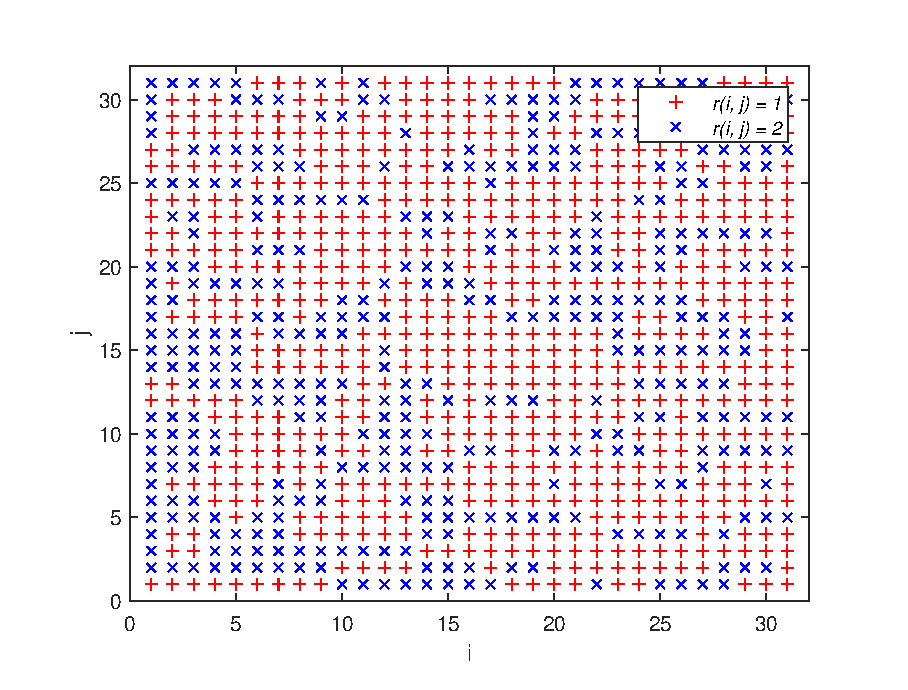
\includegraphics[scale=0.6]{./figures/2dsmc/simulations/r_eps.eps}
		\caption{系统模态变化}
		\label{fig1}
	\end{figure}
	\begin{figure}[!htb]
		\centering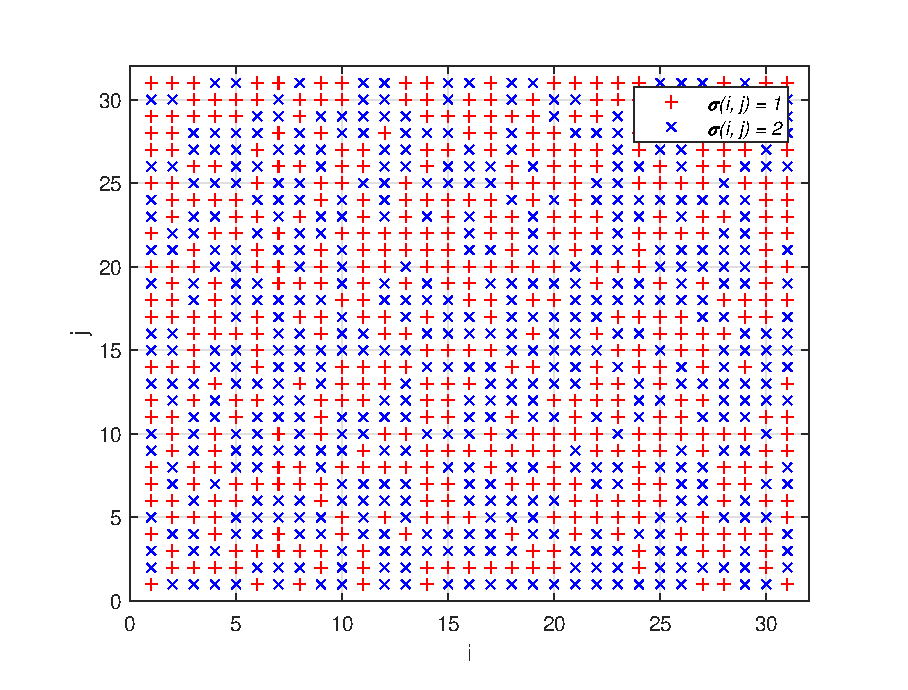
\includegraphics[scale=0.6]{./figures/2dsmc/simulations/sigma_eps.eps}\\ 
		\caption{控制器模态变化}
		\label{fig2}
	\end{figure}
	图\ref{fig1}-\ref{fig2}分别给出了一个可能的系统模态和控制器模态的演变图。通过对比,不难发现控制器的模态和系统模态是不完全匹配的。\\
	根据假设,我们设置初始条件 $X_{0}$ 和外部扰动 $w(i,j)$ 分别为
	\begin{equation*}
	\begin{aligned}
	x^{h}(0, j)&=\begin{cases}
	0.1, \quad 0\leq j \leq 10 \\
	0, \quad \ \ elsewhere
	\end{cases} \\
	x^{v}(i, 0)&=\begin{cases}
	0.1, \quad 0\leq i \leq 10 \\
	0, \quad \ \ elsewhere
	\end{cases}\\
	w(i, j)\ &=\begin{cases}
	0.2, \quad 0\leq i,j \leq 10 \\
	0, \quad \ \ elsewhere
	\end{cases}
	\end{aligned}
	\end{equation*}
	\begin{figure}[!htb]
		\centering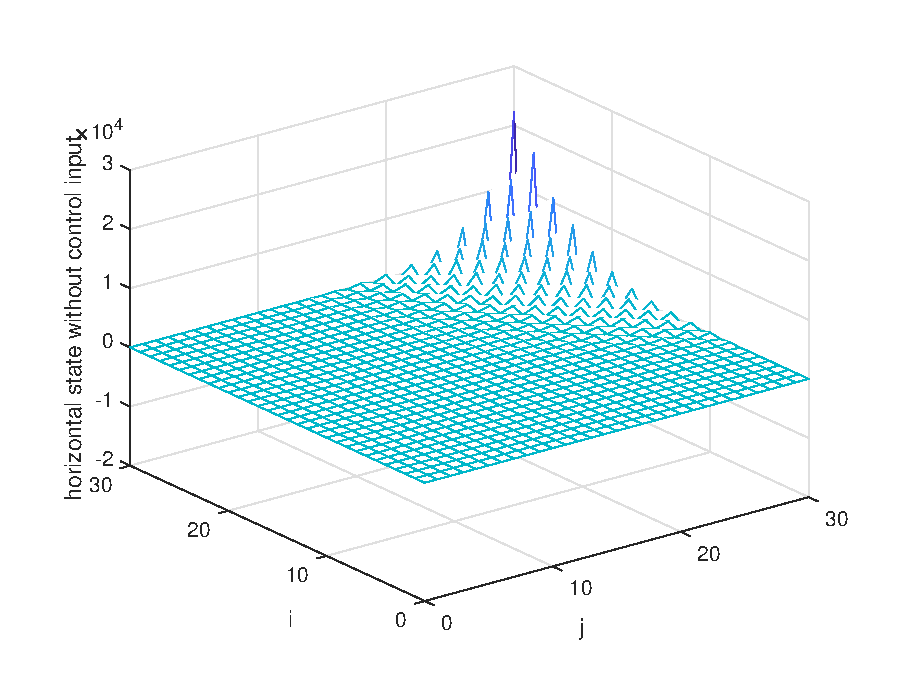
\includegraphics[scale=0.6]{./figures/2dsmc/simulations/hx-no-controll-input.eps}
		\caption{  $u(i,j)=0$时水平方向系统状态轨迹}
		\label{fig3}
	\end{figure}
	\begin{figure}[!htb]
		\centering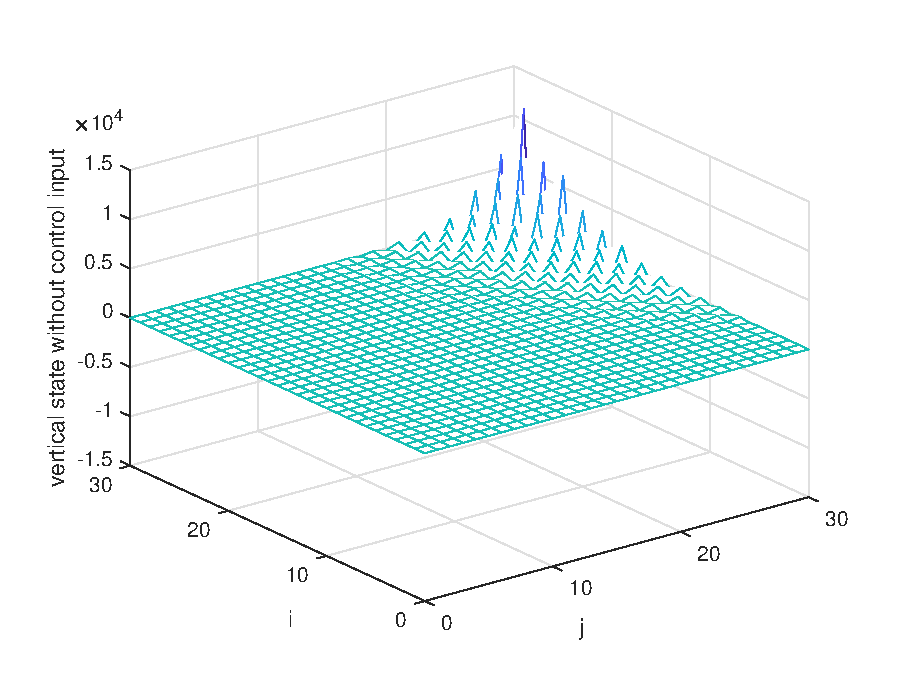
\includegraphics[scale=0.6]{./figures/2dsmc/simulations/vx-no-controll-input.eps}\\ 
		\caption{ $u(i,j)=0$时垂直方向系统状态轨迹}
		\label{fig4}
	\end{figure}
	系统 \eqref{system-equation} 在 $u(i,j) = 0$ 时系统的水平、垂直方向的系统子状态变化如图  \ref{fig3} 和\ref{fig4}。 不难看出,在不施加控制作用时,系统是不稳定的。
	然后我们按照提出的算法步骤,来进行控制器的求解。令 $\beta_{1}=0.6$ 、 $\beta_{2}=0.4$,然后求得矩阵 $G$ 为
	\begin{equation*}
	G=\begin{bmatrix}
	0.2&-0.16\\
	-0.02&-0.26
	\end{bmatrix}
	\end{equation*}
	不难验证矩阵 $GB_{k}$ 是非齐次的。参数 $\varrho_{1}$ 和 $\varrho_{2}$ 可以分别求得为 $\varrho_{1}=0.3$, $\varrho_{2}=0.6872$。 通过求解最优化问题 \eqref{optimization-problem},我们求得控制器增益为\\
	
	模态1:
	\begin{equation*}
	K_{1}=\begin{bmatrix}
	4.4147  & -4.3512\\
	-0.6827 &  -2.1886
	\end{bmatrix}
	\end{equation*}
	
	模态2:
	\begin{equation*}
	K_{2} = 	\begin{bmatrix}
	4.3706  & -3.8453 \\
	-0.6826 &  -2.3252 \\
	\end{bmatrix}
	\end{equation*}
	并且,对应的最优$H_{\infty}$ 性能为 $\gamma^{*}=0.3164$。
	\begin{figure}[!htb]
		\centering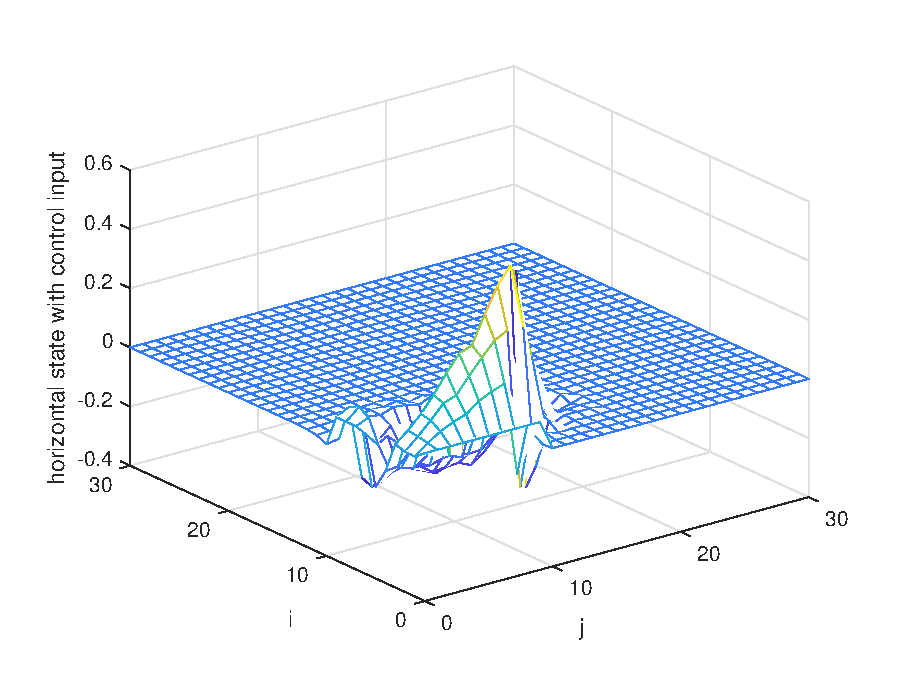
\includegraphics[scale=0.6]{./figures/2dsmc/simulations/h-state-with-force.eps}
		\caption{滑模控制器作用下的水平方向系统状态轨迹}
		\label{fig5}
	\end{figure}
	\begin{figure}[!htb]
		\centering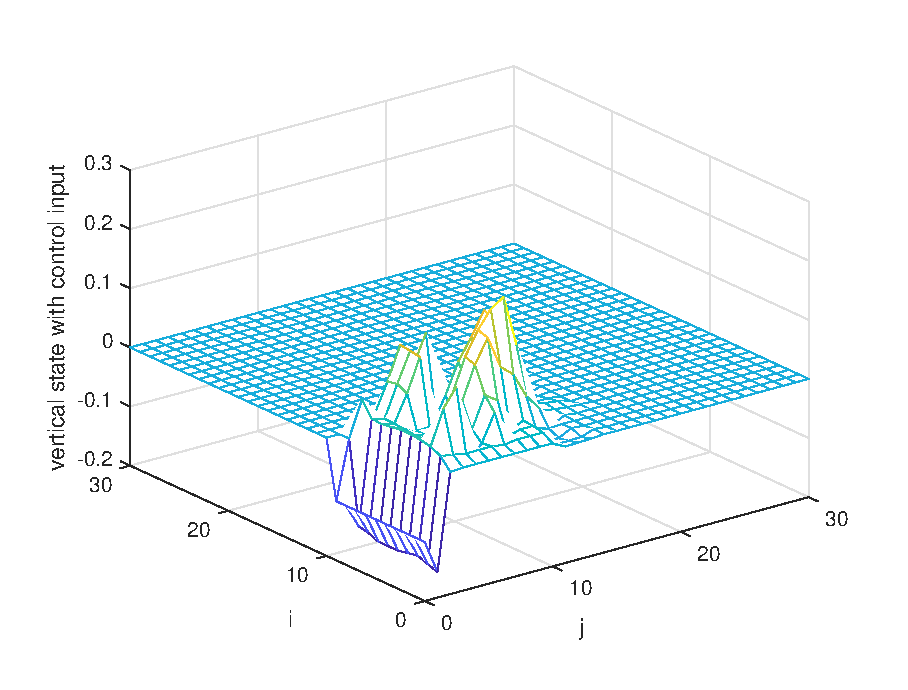
\includegraphics[scale=0.6]{./figures/2dsmc/simulations/v-state-with-force_eps.eps}\\ 
		\caption{滑模控制器作用下的垂直方向系统状态轨迹}
		\label{fig6}
	\end{figure}
	\\闭环控制系统 \eqref{closed-loop-system-equation} 在异步滑模控制器作用下的水平方向系统状态、垂直方向系统状态分别描绘在图\ref{fig5}-\ref{fig6}。显然,当施加了异步滑模控制器之后,系统状态收敛,因此系统是稳定的。可以通过条件 \eqref{siding-surface-equation} 和\eqref{smc-law}来分别求得滑模面和异步滑模控制率。 然后,图\ref{fig7}-\ref{fig10}分别给出了水平方向、垂直方向的滑模面,水平方向、垂直方向的控制输入图。 综合仿真结果,可以表明我们的异步滑模控制器是有效的。
	\begin{figure}[!htb]
		\centering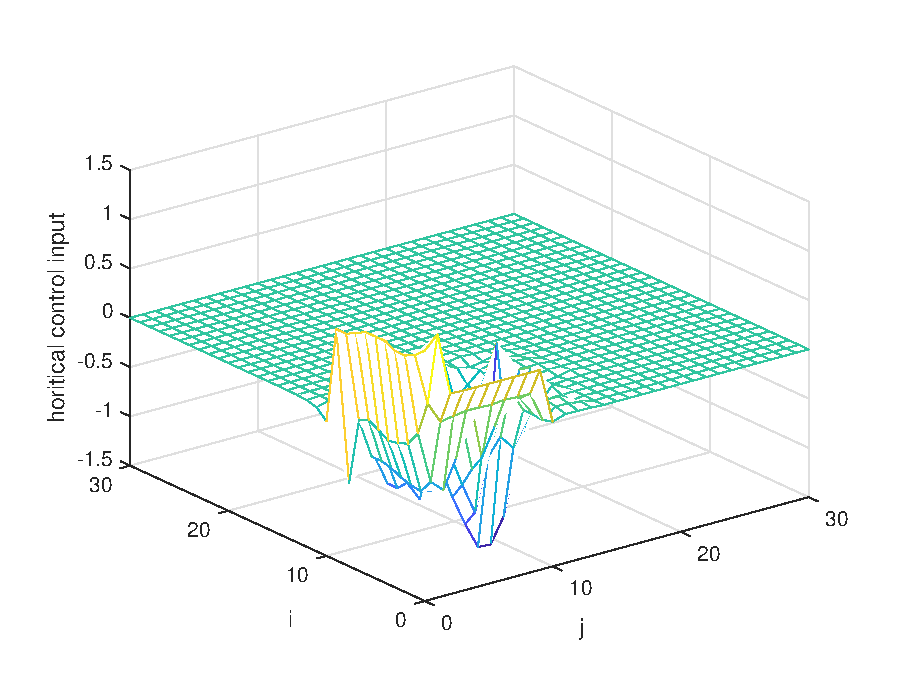
\includegraphics[scale=0.6]{./figures/2dsmc/simulations/h-control-input_eps.eps}
		\caption{水平方向异步滑模控制输入 $u^{h}(i,j)$}
		\label{fig7}
	\end{figure}
	\begin{figure}[!htb]
		\centering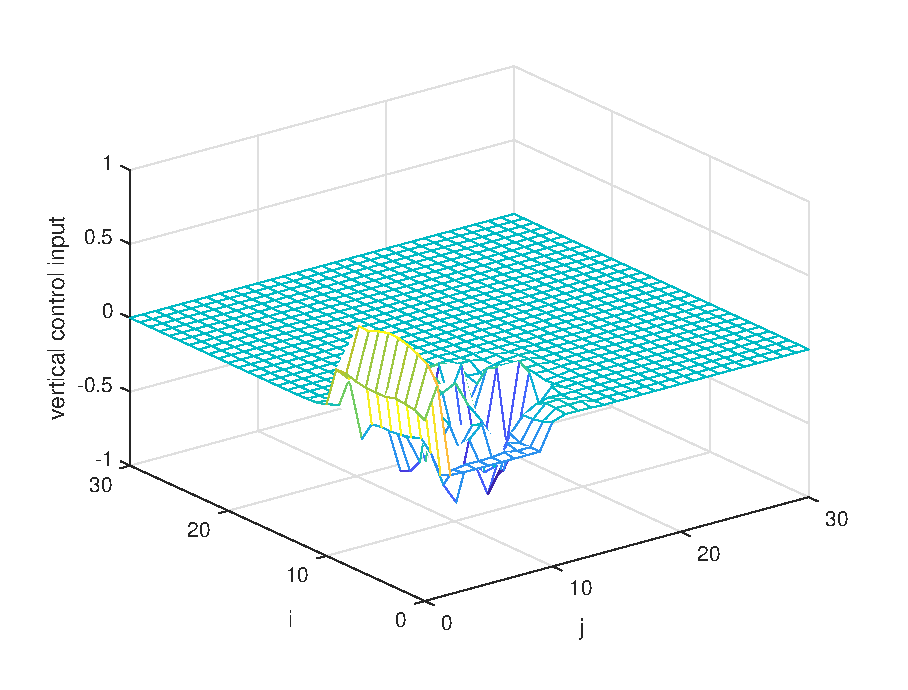
\includegraphics[scale=0.6]{./figures/2dsmc/simulations/v-controll-input_eps.eps}\\ 
		\caption{垂直方向滑模控制输入 $u^{v}(i,j)$}
		\label{fig8}
	\end{figure}
	
	\begin{figure}[!htb]
		\centering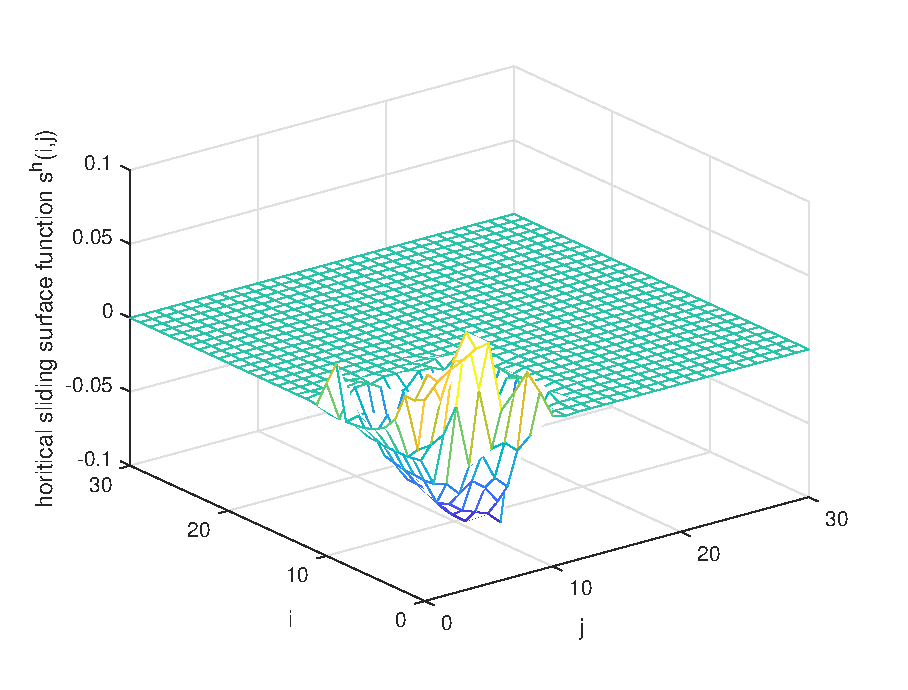
\includegraphics[scale=0.6]{./figures/2dsmc/simulations/hs_eps.eps}
		\caption{水平方向滑模面 $s^{h}(i,j)$}
		\label{fig9}
	\end{figure}
	\begin{figure}[!htb]
		\centering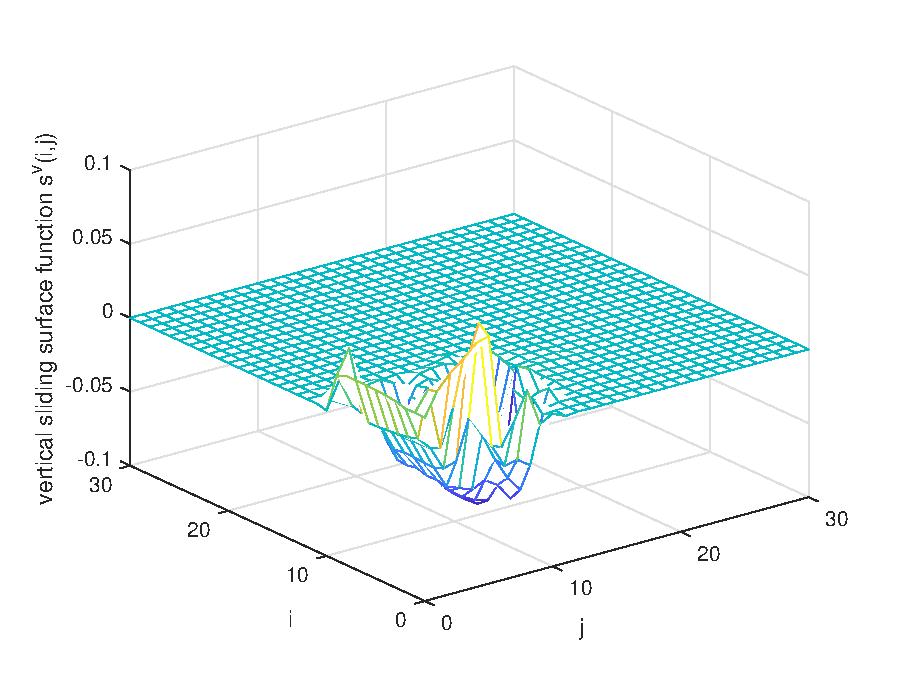
\includegraphics[scale=0.6]{./figures/2dsmc/simulations/vs_eps.eps}\\ 
		\caption{垂直方向滑模面 $s^{v}(i,j)$}
		\label{fig10}
	\end{figure}

\section{小结} \label{conclusion} 	
	本章我们研究了Roesser模型下的二维Markov跳变系统的异步滑模控制问题。考虑到控制器模态同系统模态的不匹配问题,我们基于隐Markov模型设计了异步滑模控制器。借助Lyapunov泛函方法,我们研究了系统的稳定性及其$H_{\infty}$性能,以及系统状态到滑模面的可达性问题。给出了能够使得系统稳定,且满足一定$H_{\infty}$的充分条件,同时,该条件可以保证系统状态到滑模面的可达性。最后,我们通过一个例子来验证了提出方法的有效性。
	
% !TEX root = ../thesis.tex

\chapter{二维Markov跳变系统的异步二次型控制}
这里是对Qccontrol的介绍

\section{数学模型及问题描述}
	本章考虑如下Roesser模型下的二维Markov跳变系统
	\begin{equation} \label{qc-system-equation}
	\left\{
	\begin{array}{lr}
	\hat{x}(i,j) = A_{r(i,j)}x(i,j)+B_{r(i,j)}u(i,j) \\
	z(i,j) = C_{r(i,j)}x(i,j)+D_{r(i,j)}u(i,j)
	\end{array}
	\right.
	\end{equation}
	其中,
	\begin{equation*}
	\hat{x}(i,j) = \begin{bmatrix}
	x^{h}(i+1,j) \\
	x^{v}(i,j+1)
	\end{bmatrix}, \
	x(i, j) = \begin{bmatrix}
	x^{h}(i,j) \\
	x^{v}(i,j)
	\end{bmatrix},
	\end{equation*}
	这里$x^{h}(i,j)\in\mathbb{R}^{n_1}$,$x^{v}(i,j)\in\mathbb{R}^{n_2}$分别表示水平、垂直方向的系统子状态,$u(i,j)\in\mathbb{R}^{m}$表示系统控制输入,$z(i,j)\in\mathbb{R}^{l}$表示系统被控输出。$A_{r(i,j)}$,$B_{r(i,j)}$,$C_{r(i,j)}$及$D_{r(i,j)}$是具有合适维度的已知系统时变矩阵,并且是$r(i,j)$的函数。$r(i,j)$表示一个随机跳变过程,可以用来表示Markov链,在集合$\mathcal{N}_{1} = \{1,2...N_{1}\}$中取值,并且满足具有如下状态转移概率的状态转移矩阵$\varLambda = \{\lambda_{kp}\}$
	\begin{equation}\label{qc-tps-system}
	\begin{split}
	&\Pr\{r(i+1,j)=p|r(i,j)=k\}\\
	=&\Pr\{r(i,j+1)=p|r(i,j)=k\}=\lambda_{kp},\  \forall k,p \in \mathcal{N}_{1}
	\end{split}
	\end{equation}
	且对任意的$k, p\in\mathcal{N}_{1}$,$\lambda_{kp}$ 满足
	\begin{equation}
	\left\{
	\begin{array}{lr}
	\lambda_{kp} \geq 0, \\
	\sum_{p=1}^{N_1}\lambda_{kp}=1.
	\end{array}
	\right.
	\end{equation}
	
	在实际应用系统中,由于控制器不能完全的获得系统的模态信息,因此,在本章中,我们基于隐Markov模型,设计如下异步控制器
	\begin{equation}\label{qc-controller}
	u(i,j) = K_{\sigma(i,j)}x(i,j),
	\end{equation}
	其中$K_{\sigma(i,j)}\in \mathbb{R}^{(n_1+n_2)\times m}$是待决定的控制器增益矩阵,$\sigma(i,j)$表示控制器模态,在集合$\mathcal{N}_{2} = \{1,2...N_{2}\}$中取值,并且满足具有如下条件状态转移概率的状态转移矩阵 $\varPsi=\{\mu_{k\tau }\}$
	\begin{equation}
	\Pr\{\sigma(i,j)=s|r(i,j)=k\}=\mu_{ks }, %\forall  k\in\mathcal{N}_{1}, \tau\in\mathcal{N}_{2},
	\end{equation}
	且,对任意的$k\in\mathcal{N}_{1}, s\in\mathcal{N}_{2}$,有 $\mu_{k\tau }\in[0,1]$,对任意的$k$,有  $\sum_{s =1}^{N_{2}}\mu_{ks } = 1$。
	
	然后,在本章中,我们对初始条件($X_{0},\varGamma_{0}$)定义如下:
	\begin{equation*}
		\left\{
			\begin{array}{lr}
				X_{0}\equiv \big\{x^{h}(0,0),x^{h}(0,1),x^{h}(0,2),\cdots, x^{v}(0,0),x^{v}(1,0),x^{v}(2,0),\cdots  \big\},\\
				\varGamma_{0}\equiv \big\{r(0,0), r(0,1),r(0,2),\cdots,r(1,0),r(2,0),\cdots \big\}.
			\end{array}
		\right.
	\end{equation*}
	
	下面,我们对初始状态$X_{0}$做下面几个假设:
	
	{\bf 假设 \ \ 4.1:}
	2D系统\eqref{qc-system-equation}的零初始状态为,对任意的非负整数$i,j$,有$x^{h}(0,j) =0, x^{v}(i,0)=0$。
	
	{\bf 假设 \ \ 4.2:}
	系统\eqref{qc-system-equation}的初始状态$X_{0}$满足
	\begin{equation}
	\mathscr{X}_{0} \equiv \lim\limits_{L\to\infty}\mathbb{E}\Big\{\sum_{l=1}^{L}(\|x^{h}(0,l)\|^{2}+ \|x^{v}(l,0)\|^{2})\Big\} < \infty
	\end{equation}
	这里 $\mathbb{E}\{\cdot\}$ 表示数学期望,且,我们称系统的全部初始状态之和是有界的。
	
	{\bf 假设 \ \ 4.3:}
	在假设4.2的基础上,我们进一步假设,存在两个正整数$l_1$,$l_2$,使得
	\begin{equation}
		\left\{
		\begin{array}{lr}
		x^{h}(0,j)=0,\quad j\geq l_1,\\
		x^{v}(i,0)=0,\quad i\geq l_2.
		\end{array}
		\right.
	\end{equation}
	此时,系统只有有限个非零初始状态。
	
	{\bf 假设 \ \ 4.4:}
	在假设4.3的基础上,我们进一步做如下假设。存在$L(0,j)$,$L(i,0)$,$Z_1$,$Z_2$,使得对任意的$j<l_1,i<l_2$有
	\begin{equation}
		\left\{
		\begin{array}{lr}
		x^{h}(0,j)=Z_1L(0,j),\quad L^{T}(0,j)L(0,j)\leq 1,\\
		x^{v}(i,0)=Z_2L(i,0),\quad  L^{T}(i,0)L(i,0)\leq 1.
		\end{array}
		\right.
	\end{equation}
	此时,我们称系统的只有有限个非零初始状态,且每一个非零初始状态都是有界的。
	
	{\bf 注 \ \ 4.1:}
	实际上,不难发现,对于任意给定的$x^{h}(0,j)$,$x^{v}(i,0)$,我们总是可以通过选择合适的$Z_1$,$Z_2$及$L(0,j)$,$L(i,0)$对其进行表示。这个初始条件的假设思路已经在文献[123]中使用了,不过,值得注意的是,在上述文献中,都假设水平、垂直状态的初始状态是分别一样的,而在我们的假设中,并没有这么强的约束,因此更加贴近实际情况。
	
	下面,我们给出系统\eqref{qc-system-equation}的稳定性及成本函数的定义
	
	{\bf 定义 \ \ 4.1:}
	如果下式对任意的初始条件$X_{0}$成立
	\begin{equation}\label{qc-AMSS}
	\lim\limits_{i+j\to\infty}\mathbb{E}\{\|x(i,j)\|^{2}\} = 0
	\end{equation}
	我们称,在假设4.1意义下的系统\eqref{qc-system-equation}是渐进均方稳定的。
	
	本章中,我们考虑如下成本函数
	\begin{equation}\label{qccostfuntion}
	\begin{split}
	J(i,j) \equiv \|z\|_{2}^{2} = \sum_{i=0}^{\infty}\sum_{j=0}^{\infty}E(\|z(i,j)\|^{2})\\
	\end{split}
	\end{equation}
	
	由系统\eqref{qc-system-equation}及控制器\eqref{qc-controller}可以得到闭环2D控制系统的方程为
	\begin{equation}\label{qc-closed-system-equation}
		\left\{
			\begin{array}{lr}
				\hat{x}(i,j) = (A_{r(i,j)}+B_{r(i,j)}K_{\sigma(i,j)})x(i,j), \\
				z(i,j) = (C_{r(i,j)}+D_{r(i,j)}K_{\sigma(i,j)})x(i,j).
			\end{array}
		\right.
	\end{equation}
	
	本章的目标为,设计异步控制器$K_{\sigma(i,j)}$,使得闭环控制系统渐进均方稳定,且满足一定的保成本性能$J^{*}$,针对初始条件的不同,我们分为下面三种情况进行讨论
	
	(1) 初始状态$X_{0}$已知(假设4.3成立),且初始模态$\varGamma_{0}$已知。
	
	(2) 初始状态$X_{0}$未知,但满足假设4.4,且初始模态$\varGamma_{0}$已知。
	
	(3) 初始状态$X_{0}$未知,但满足假设4.4,且初始模态$\varGamma_{0}$未知。
	

\section{主要结论}
	在本节,我们首先探究闭环控制系统\eqref{qc-closed-system-equation}的稳定性问题,然后,针对初始条件$(X_{0}, \varGamma_{0})$的三种不同情况,分别讨论他们的保成本性能。
	
	{\bf 定理 \ \ 4.1:} 
	考虑闭环控制系统\eqref{qc-closed-system-equation},当系统初始状态满足假设4.3,且系统初始模态已知时候,若对任意的$k\in\mathcal{N}_{1}$,$s\in\mathcal{N}_2$,存在正定矩阵$R_{k}=\mathrm{diag}\{R^{h}_{k},R^{v}_{k}\}$,$Q_{ks}$,矩阵$K_{s}$,使得下列不等式成立,
	\begin{equation}\label{qc-T1-1}
	\sum_{s=1}^{N_2}u_{ks}Q_{ks}-R_{k}< 0,
	\end{equation}
	\begin{equation}\label{qc-T1-2}
	\bar{A}^{T}_{ks}\mathcal{R}_{k}\bar{A}_{ks}+\bar{C}^{T}_{ks}\bar{C}_{ks}-Q_{ks}<0,
	\end{equation}
	其中,$\bar{A}_{ks}=A_{k}+B_kK_s$,$\bar{C}_{ks}=C_k+D_kK_s$,$\mathcal{R}_{k}=\sum_{s =1}^{N_1}\lambda_{kp}R_p$。则,系统是渐进均方稳定的,且,相对应的保成本性能为
	\begin{equation}\label{qcT1C3}
		J(i,j)\leq  \sum_{j=0}^{l_1-1}V_{1}(0,j)+\sum_{i=0}^{l_2-1}V_2(i,0).
	\end{equation}
	其中,$V_{1}(i,j)$ 及 $V_{2}(i,j)$ 定义如下  
	\begin{equation*}
	\left\{
	\begin{array}{lr}
	\begin{split}
	V_{1}(i,j)=x^{hT}(i,j)R^{h}_{r(i,j)}x^{h}(i,j),\\
	V_{2}(i,j)=x^{vT}(i,j)R^{v}_{r(i,j)}x^{v}(i,j).
	\end{split}
	\end{array}
	\right.
	\end{equation*}
	{\bf 证明:} 
	首先,我们选择如下李雅普诺夫函数,
	\begin{equation*}
		V(i,j) = x^{T}(i,j)R_{r(i,j)}x(i,j)
	\end{equation*}
	令
	\begin{equation*}
	\hat{V}(i,j) = \hat{x}^{T}(i,j)\mathrm{diag}\{R^{h}_{r(i+1,j)},R^{v}_{r(i,j+1)}\}\hat{x}(i,j)
	\end{equation*}
	那么,由闭环控制系统\eqref{qc-closed-system-equation}和转移概率函数\eqref{qc-tps-system},我们可以推出
	\begin{equation}\label{qc-diff1}
		\begin{split}
			\mathbb{E}\{\varDelta V(i,j)\}&=\mathbb{E}\{\hat{V}(i,j)-V(i,j) \}\\
				&=\mathbb{E}\{\hat{x}^{T}(i,j)\mathcal{R}_{k}\hat{x}(i,j) \}- x^{T}(i,j)R_{k}x(i,j)\\
				&= x^{T}(i,j)\{\sum_{s=1}^{N_2}u_{ks} \bar{A}^{T}_{ks}\mathcal{R}_{k}\bar{A}_{ks} -R_{k} \}x(i,j)  
		\end{split}
	\end{equation}
	由\eqref{qc-T1-1}-\eqref{qc-T1-2},我们可以得到
	\begin{equation}\label{qc-dif1}
		\sum_{s =1}^{N_2}u_{ks}\bar{A}^{T}_{ks}\mathcal{R}_{k}\bar{A}_{ks}-R_{k}<0
	\end{equation}
	因此,由\eqref{qc-diff1}-\eqref{qc-dif1},我们可以进一步推出
	\begin{equation}\label{qc18}
		\mathbb{E}\{\varDelta V(i,j)\} < -\alpha \mathbb{E}\{\|x(i,j)\|^{2} \}
	\end{equation}
	这里,$\alpha$表示$(R_{k}-\sum_{s =1}^{N_2}u_{ks}\bar{A}^{T}_{ks}\mathcal{R}_{k}\bar{A}_{ks})$的最小特征值。显然,$\alpha$是一个正数。对\eqref{qc18}两边做累加,我们可以推出
	\begin{equation}
		\mathbb{E}\{ \sum_{i=0}^{l_2-1}\sum_{j=0}^{l_1-1}\|x(i,j)\|^{2} \}<-\frac{1}{\alpha}\mathbb{E}\{\sum_{i=0}^{l_2-1}\sum_{j=0}^{l_1-1}\varDelta V(i,j) \}
	\end{equation}
	这里,$l_1$,$l_2$已经定义在假设4.3中。接下来,我们使用$R_{k}=\mathrm{diag}\{R^{h}_{k},R^{v}_{k}\}$,$\mathbb{E}\{\varDelta V(i,j)\}=\mathbb{E}\{\hat{V}(i,j)-V(i,j) \}$,将水平,垂直状态分开,可以推出
	\begin{equation} \label{qc19}
	\begin{split}
	&\sum_{i=0}^{l_2-1}\sum_{j=0}^{l_1-1}  \varDelta V(i,j)\\&= \sum_{i=0}^{l_2-1}\big\{V_2(i,l_1) - V_2(i,0) \big\}+  \sum_{j=0}^{l_1-1}\big\{V_1(l_2,j) - V_1(0,j) \big\}\\
	&\leq -\big( \sum_{i=0}^{l_2-1}V_2(i,0) + \sum_{j=0}^{l_1-1}V_{1}(0,j)\big) \\
	%			&\leq -\beta \sum_{\ell=0}^{\infty} \big(  \|x^{v}(\ell,0)\|^{2} + \|x^{h}(0,\ell)\|^{2} \big)
	\end{split}
	\end{equation} 
	由\eqref{qc18}-\eqref{qc19}可以推出
	\begin{equation}\label{qc20}
	\begin{split}
	\mathbb{E}\Big\{\sum_{i=0}^{\infty}\sum_{j=0}^{\infty}  \|x(i,j)\|^{2} \Big\} &\leq \frac{\beta}{\alpha} \sum_{\ell=0}^{\infty} \big(  \|x^{v}(\ell,0)\|^{2} + \|x^{h}(0,\ell)\|^{2} \big)<\infty
	\end{split}	
	\end{equation}
	这里的$\beta$是$R^{h}_{r(i,j)}$,$R^{v}_{r(i,j)}$的最大特征值。显然,上式可以保证\eqref{qc-AMSS}成立,因此,研究的系统是渐进均方稳定的。
	现在,我们对成本性能进行分析,由\eqref{qc-T1-1}-\eqref{qc-T1-2},可以推出
	\begin{equation}
		\begin{split}
			\mathbb{E}\{\|z(i,j)\|^{2}+\varDelta V(i,j) \}=x^{T}(i,j)\{\sum_{s=1}^{N_2}u_{ks} \bar{A}^{T}_{ks}\mathcal{R}_{k}\bar{A}_{ks} +C^{T}_{ks}C_{ks}-R_{k} \}x(i,j)<0
		\end{split}
	\end{equation}
	对上式做累加得到
	\begin{equation}
	\begin{split}
	&\sum_{i=0}^{\infty}\sum_{j=0}^{\infty}\mathbb{E}\{\|z(i,j)\|^{2}+\varDelta V(i,j) \}\\&=J(i,j)+\sum_{i=0}^{\infty}\sum_{j=0}^{\infty}\mathbb{E}\{\varDelta V(i,j) \}\\
	&<J(i,j)-\big( \sum_{i=0}^{l_2-1}V_2(i,0) + \sum_{j=0}^{l_1-1}V_{1}(0,j)\big)\\&<0
	\end{split}
	\end{equation}
	因此,
	\begin{equation}
		J(i,j)<\big( \sum_{i=0}^{l_2-1}V_2(i,0) + \sum_{j=0}^{l_1-1}V_{1}(0,j)\big)
	\end{equation}
	至此,定理证明结束。
	
	{\bf 注 \ \ 4.2:}
	仔细检查定理4.1的推导,我们不难发现,其实,假设4.2即可以保证闭环控制系统的稳定性。


	{\bf 定理 \ \ 4.2:}
	考虑闭环控制系统\eqref{qc-closed-system-equation},当系统初始状态满足假设4.4,初始模态已知时,若对任意的$k\in\mathcal{N}_{1}$,$s\in\mathcal{N}_2$,存在正定矩阵$R_{k}=\mathrm{diag}\{R^{h}_{k},R^{v}_{k}\}$,$Q_{ks}$,矩阵$K_{s}$,使得不等式\eqref{qc-T1-1}-\eqref{qc-T1-2}成立,则,系统是渐进均方稳定的,且,相对应的保成本性能为
	\begin{equation}\label{qcT2}
	\begin{split}
	J(i,j) \leq \sum_{\varrho_{1}=1}^{N_{1}}\varpi_{\varrho_{1}}\lambda_{max}(Z^{T}_{1}R^{h}_{\varrho_{1}}Z_{1})
	+\sum_{\varrho_{2}=1}^{N_{1}}\omega_{\varrho_{2}}\lambda_{max}(Z^{T}_{2}R^{v}_{\varrho_{2}}Z_{2})
	\end{split}
	\end{equation}
	这里,$\varrho_{1}$,$\varrho_{2}$分别表示系统、控制器的模态,$\varpi_{\varrho_{1}}$,$\omega_{\varrho_{2}}$分别表示初始模态中,对应的系统模态等于$\varrho_{1}$,控制器模态等于$\varrho_{2}$的数量。
	
	{\bf 证明:} 
	我们选择跟定理4.1一样的李雅普诺夫函数,稳定性不难发现已经可以由\eqref{qc-T1-1}-\eqref{qc-T1-2}保证。同时,由假设4.4是假设4.3基础上的进一步加强,则易可以知道,在假设4.4的基础上,可以保证\eqref{qcT1C3}成立。由假设4.4,我们可以推出
	\begin{equation}
		\begin{split}
			J(i,j)&\leq \varpi_1\lambda_{max}(Z^{T}_{1}R^{h}_{1}Z_{1})+\dots+\varpi_{N_{1}}\lambda_{max}(Z^{T}_{1}R^{h}_{N_{1}}Z_{1}) \\ 
			&+\omega_{1}\lambda_{max}(Z^{T}_{2}R^{v}_{1}Z_{2})+\dots+\omega_{N_{2}}\lambda_{max}(Z^{T}_{2}R^{v}_{N_2}Z_{2})\\
			&=\sum_{\varrho_{1}=1}^{N_{1}}\varpi_{\varrho_{1}}\lambda_{max}(Z^{T}_{1}R^{h}_{\varrho_{1}}Z_{1})
			+\sum_{\varrho_{2}=1}^{N_{1}}\omega_{\varrho_{2}}\lambda_{max}(Z^{T}_{2}R^{v}_{\varrho_{2}}Z_{2})
		\end{split}
	\end{equation}
	至此,证明完毕。
	
	{\bf 定理 \ \ 4.3:}
	考虑闭环控制系统\eqref{qc-closed-system-equation},当系统初始状态满足假设4.4,初始模态未知时,若对任意的$k\in\mathcal{N}_{1}$,$s\in\mathcal{N}_2$,存在正定矩阵$\bar{R}_{k}=\mathrm{diag}\{\bar{R}^{h}_{k},\bar{R}^{v}_{k}\}$,$\bar{Q}_{ks}$,矩阵$\bar{K}_{s}$,$T_{s}$,使得下列不等式成立
	\begin{equation}\label{qcT3C1}
	\begin{bmatrix}
	-\lambda_1I &Z^{T}_1\\
	*&-\bar{R}^{h}_{k}
	\end{bmatrix}<0
	\end{equation}
	\begin{equation}\label{qcT3C2}
	\begin{bmatrix}
	-\lambda_2I &Z^{T}_{2}\\
	*&-\bar{R}^{v}_{k}
	\end{bmatrix}<0
	\end{equation}
	\begin{equation}\label{qcT3C3}
	\begin{bmatrix}
	-\bar{R}_{k}& \sqrt{u_{k1}}\bar{R}_{k} &\cdots&\sqrt{u_{kN_2}}\bar{R}_{k}\\
	*&-\bar{Q}_{k1}&\cdots&0\\
	*&*&\ddots&0\\
	*&*&*&-\bar{Q}_{kN_2}\\
	\end{bmatrix}<0
	\end{equation}
	\begin{equation}\label{qcT3C4}
	\begin{bmatrix}
		\bar{Q}_{ps}-T_{s}-T^{T}_{s} & C_{k}T_s+D_k\bar{K}_s& \sqrt{\lambda_{k1}}(A_kT_s+B_k\bar{K}_s)&\cdots&\sqrt{\lambda_{kN_1}}(A_kT_s+B_k\bar{K}_s)\\
				*&-I&0&\cdots&0\\
				*&*&-\bar{R}_1&\cdots&0\\
				\vdots&\vdots&\vdots&\ddots&0\\
				*&*&*&*&-\bar{R}_{N_1}\\
				
	\end{bmatrix}<0
	\end{equation}	
	则,系统是渐进均方稳定的,且,相对应的保成本性能为
	\begin{equation}
	\begin{split}
	J(i,j) \leq l_1\lambda_1 + l_2\lambda_2
	\end{split}
	\end{equation}
	{\bf 证明:} 定义$\bar{R}_{k}=R^{-1}_{k}$,$\bar{Q}_{ks}=Q^{-1}_{ks}$,$\bar{K}_s=K^{-1}_s$。
	对\eqref{qcT3C3}两边同时灯以$\mathrm{diag}\{R^{k},I,\dots,I \}$,可以得到
	\begin{equation} 
	\begin{bmatrix}
	-R_{k}& \sqrt{u_{k1}}R_{k} &\cdots&\sqrt{u_{kN_2}}R_{k}\\
	*&-\bar{Q}_{k1}&\cdots&0\\
	*&*&\ddots&0\\
	*&*&*&-\bar{Q}_{kN_2}\\
	\end{bmatrix}<0
	\end{equation}
	然后,根据Schur补引理,可以得到可以得到\eqref{qc-T1-1}。
	不难发现\eqref{qcT3C4}可以推出下式
	\begin{equation} 
	\begin{bmatrix}
	T^{T}_{s}\bar{Q}_{ps}T_{s} & C_{k}T_s+D_k\bar{K}_s& \sqrt{\lambda_{k1}}(A_kT_s+B_k\bar{K}_s)&\cdots&\sqrt{\lambda_{kN_1}}(A_kT_s+B_k\bar{K}_s)\\
	*&-I&0&\cdots&0\\
	*&*&-\bar{R}_1&\cdots&0\\
	\vdots&\vdots&\vdots&\ddots&0\\
	*&*&*&*&-\bar{R}_{N_1}\\
	\end{bmatrix}<0
	\end{equation}
	使用$\mathrm{diag}\{T^{-1}_s,I,\dots,I \}$分别左乘,右乘上式,然后使用Schur补引理,可以推出\eqref{qc-T1-2}成立。
	这样,系统的稳定性可以保证。
	根据假设4.3,由于系统的初始模态并不知道,我们无法确定系统每个模态对应的数量。因此,我们需要对任意的系统模态下,$\lambda_{max}(Z^{T}_{1}R^{h}_{\varrho_{1}}Z_{1})$,$\lambda_{max}(Z^{T}_{2}R^{v}_{\varrho_{2}}Z_{2})$分别得到确定一个统一的上界。
	由\eqref{qcT3C1}-\eqref{qcT3C2}可以得到
	\begin{equation}
		\begin{split}
			&Z^{T}_1R^{h}_{k}Z_1<\lambda_1I,\\ &Z^{T}_2R^{v}_{k}Z_2<\lambda_2I	
		\end{split}
	\end{equation}
	这里,$\lambda_1$是对全部系统模态,$\lambda_{max}(Z^{T}_{1}R^{h}_{\varrho_{1}}Z_{1})$的上界,$\lambda_2$是对全部系统模态,$\lambda_{max}(Z^{T}_{2}R^{v}_{\varrho_{2}}Z_{2})$的上界。
	因此,由\eqref{qcT2}可以推出
	\begin{equation}
		J(i,j) \leq l_1\lambda_1 + l_2\lambda_2
	\end{equation}
	至此,定理证明完毕。
	
	{\bf 注 \ \ 4.2:}
	本章中,可以先通过下面的最优化问题求解出$\bar{K}_s$
	\begin{equation}\label{qc_optimization-problem}
	\text{min $(l_1\lambda_1 + l_2\lambda_2)$ subject to \eqref{qcT3C1}-\eqref{qcT3C4}}。
	\end{equation}
	然后通过$K_s=\bar{K}_sT^{-1}_s$来求解出异步控制器增益。

\section{数值例子}
	在本节,我们将选择一个简单的数值仿真例子,来验证设计的异步二次型控制器的有效性。首先,我们选择控制器模态、系统模态都为2,即$N_1=N_2=2$。然后选择系统参数如下
	
	模态一:
	\begin{equation} \notag
	\begin{aligned}
	A_{1} &= \begin{bmatrix}
	-1.0&0.6\\
	-0.2&-1.3
	\end{bmatrix}, \ 
	B_{1} = \begin{bmatrix}
	0.2&0.1\\ 1.2&0.8
	\end{bmatrix} ,\
		C_{1} &= \begin{bmatrix}
	1&0\\1.2&0.8
	\end{bmatrix},\
	D_{1} = \begin{bmatrix}
	-0.1&0\\0&0.1
	\end{bmatrix}
	\end{aligned}  
	\end{equation}
	
	模态二:
	\begin{equation} \notag
	\begin{aligned}
	A_{2} &= \begin{bmatrix}
	-1.2&0.6\\
	-0.4&-1.2
	\end{bmatrix}, \ 
	B_{2} = \begin{bmatrix}
	0.3&0.2\\ 1.0&0.8
	\end{bmatrix} ,\
	C_{2} &= \begin{bmatrix}
	1.2&0\\1.0&0.8
	\end{bmatrix},\
	D_{2} = \begin{bmatrix}
	-0.1&0\\0&0.1
	\end{bmatrix}
	\end{aligned}  
	\end{equation}
	
	系统的模态转移矩阵$\varPi$、控制器的条件模态转移矩阵$\varPsi$分别设置为
	\begin{equation}
		\varPi = \begin{bmatrix}
		0.8& 0.2\\ 0.3& 0.7
		\end{bmatrix},    %system mode transfer function.
		\varPsi = \begin{bmatrix}
			0.6& 0.4\\0.4 &0.6
		\end{bmatrix}
	\end{equation}
	
	
	初始状态我们设置为:
	\begin{equation*}
	\begin{aligned}
	x^{h}(0, j)&=\begin{cases}
	0.1, \quad 0\leq j \leq 10 \\
	0, \quad \ \ elsewhere
	\end{cases} \\
	x^{v}(i, 0)&=\begin{cases}
	0.1, \quad 0\leq i \leq 10 \\
	0, \quad \ \ elsewhere
	\end{cases}
	\end{aligned}
	\end{equation*}
	
	根据假设4.4,我们不难发现,对任意的$i\leq10,j\leq10$,可以选择$L(i,0)=L(0,j)=1$,相应的$Z_1=Z_2=0.1$。
	
	当没有施加异步控制器时,系统在水平方向、垂直方向的状态轨迹分别绘制于图\ref{figqchstate}、图\ref{figqcvstate}中。不难发现,当$u(i,j)=0$,即不施加控制反馈作用时,系统水平方向、垂直方向的状态轨迹都是离散的,表明,此时系统不稳定。
	
	\begin{figure}[!htb]
		\centering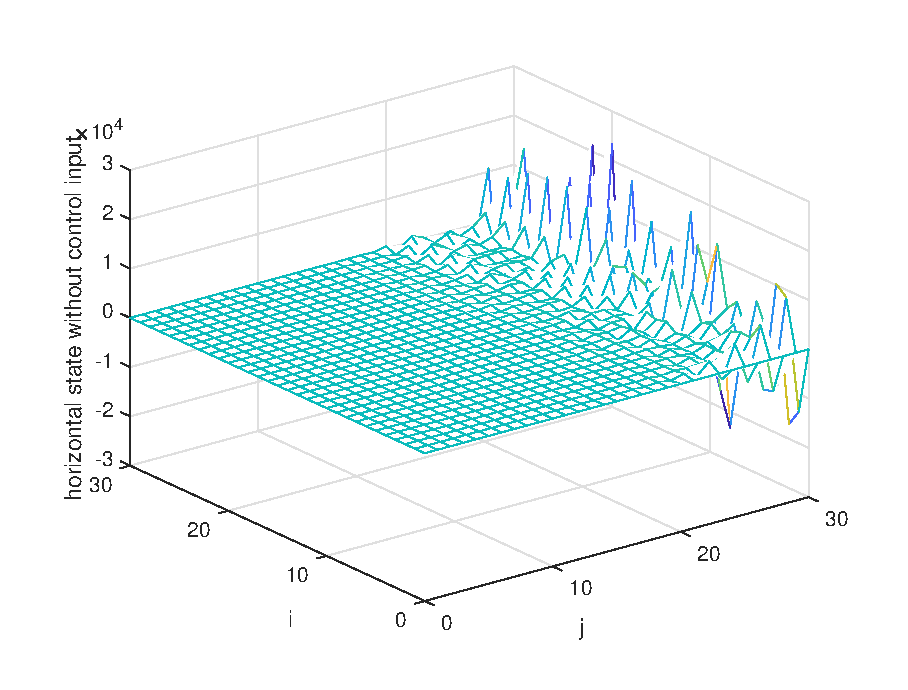
\includegraphics[scale=0.6]{./figures/qc/simulation/hstateU0.eps}\\ 
		\caption{$u(i,j)=0$时的水平状态 $x^{h}(i,j)$}
		\label{figqchstate}
	\end{figure}
	
	\begin{figure}[!htb]
		\centering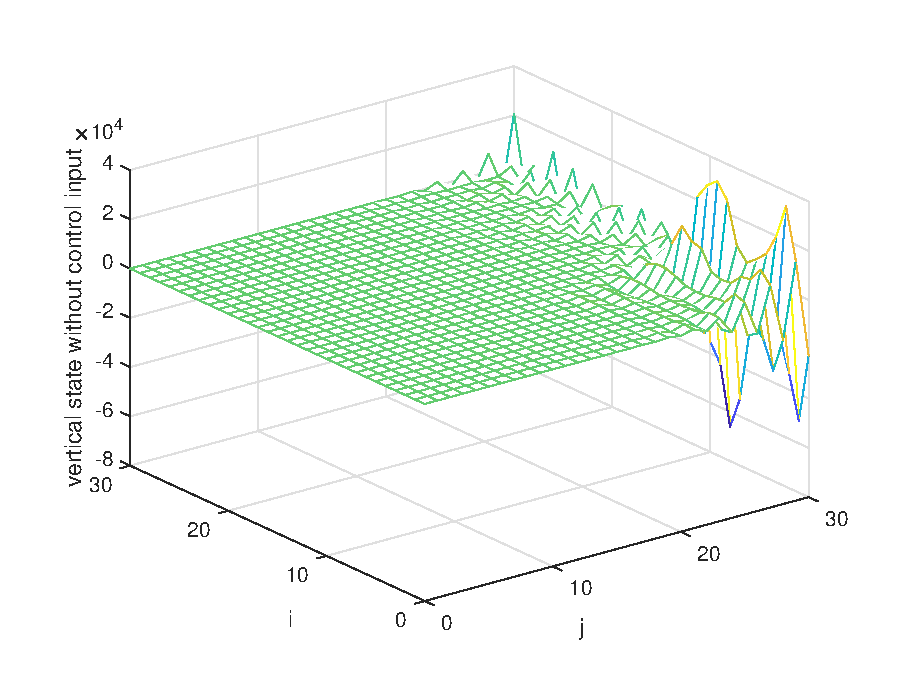
\includegraphics[scale=0.6]{./figures/qc/simulation/vstateU0.eps}\\ 
		\caption{$u(i,j)=0$时的垂直状态 $x^{v}(i,j)$}
		\label{figqcvstate}
	\end{figure}
	
	下面我们通过求解最优化问题\eqref{qc_optimization-problem},可以得到如下控制器矩阵增益
	
	模态一:
	\begin{equation*}
	K_{1}=\begin{bmatrix}
	 6.1883   &-2.0444\\
	-5.5118   &-3.4863
	\end{bmatrix}
	\end{equation*}
	
	模态二:
	\begin{equation*}
	K_{2} = 	\begin{bmatrix}
	6.5645   &-0.8006\\
	-5.5108   &-4.2340
	\end{bmatrix}
	\end{equation*}
	
	同时,系统的最小保成本性能$J^{*}=0.4512$。然后,施加了控制器以后的系统水平、垂直状态轨迹分别绘制于图\ref{figqchstate1}、图\ref{figqcvstate1}中。显然,当施加了异步二次型控制器以后,系统在水平、垂直方向的状态轨迹都收敛了,表明,此时系统是稳定的。同时,控制作用$u(i,j)$在水平方向、垂直方向的作用效果分别绘制于图\ref{figqcuh}、图\ref{figqcuv}中。综合仿真结果,可以得出结论,我们设计的控制器是有效的。
	\begin{figure}[!htb]
		\centering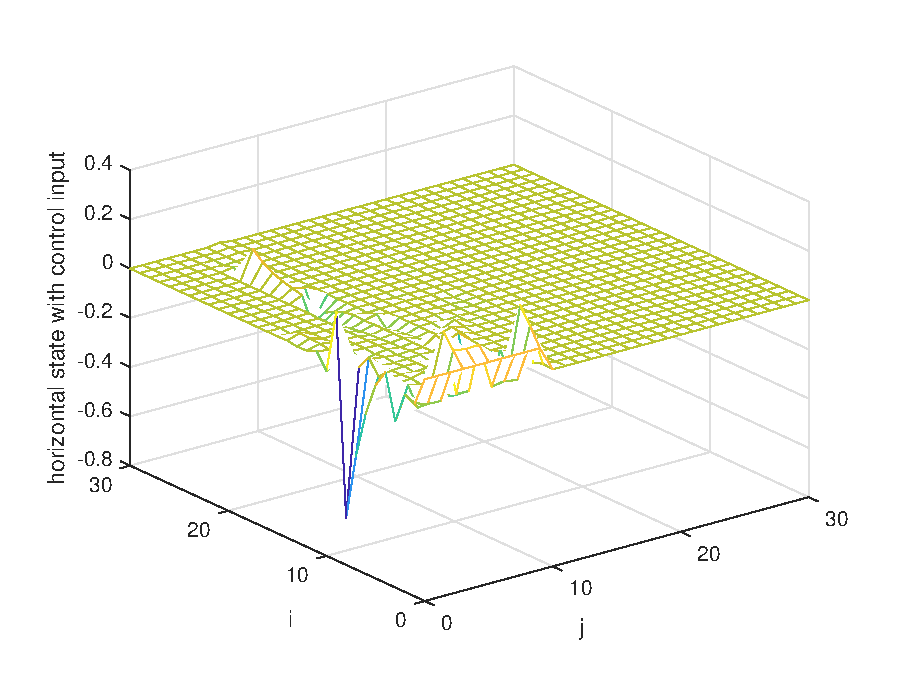
\includegraphics[scale=0.6]{./figures/qc/simulation/hstate.eps}\\ 
		\caption{异步二次型控制下的水平状态 $x^{h}(i,j)$}
		\label{figqchstate1}
	\end{figure}
	
	\begin{figure}[!htb]
		\centering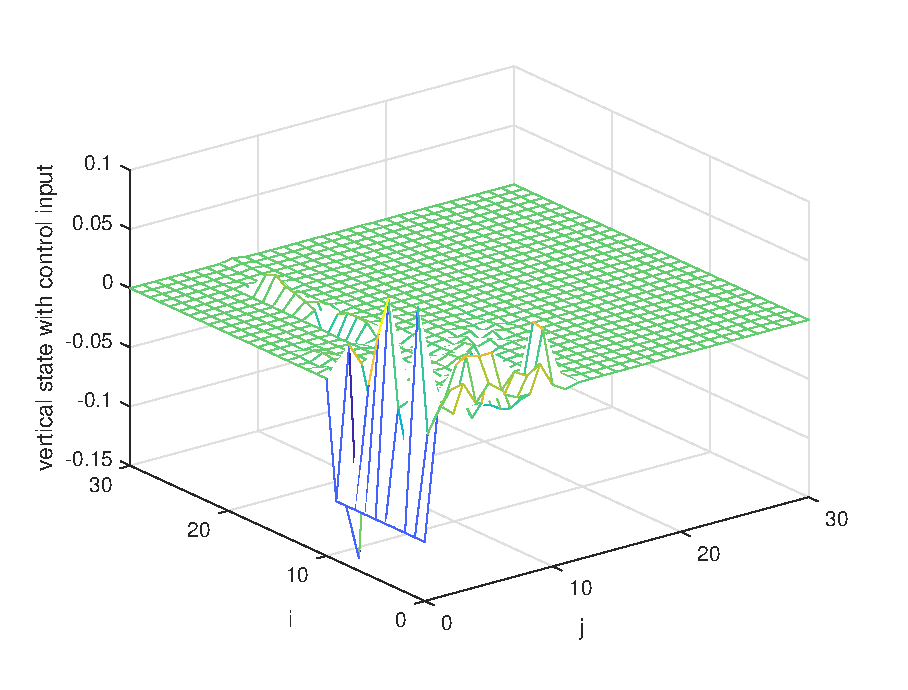
\includegraphics[scale=0.6]{./figures/qc/simulation/vstate.eps}\\ 
		\caption{异步二次型控制下的垂直状态 $x^{v}(i,j)$}
		\label{figqcvstate1}
	\end{figure}
	
	\begin{figure}[!htb]
		\centering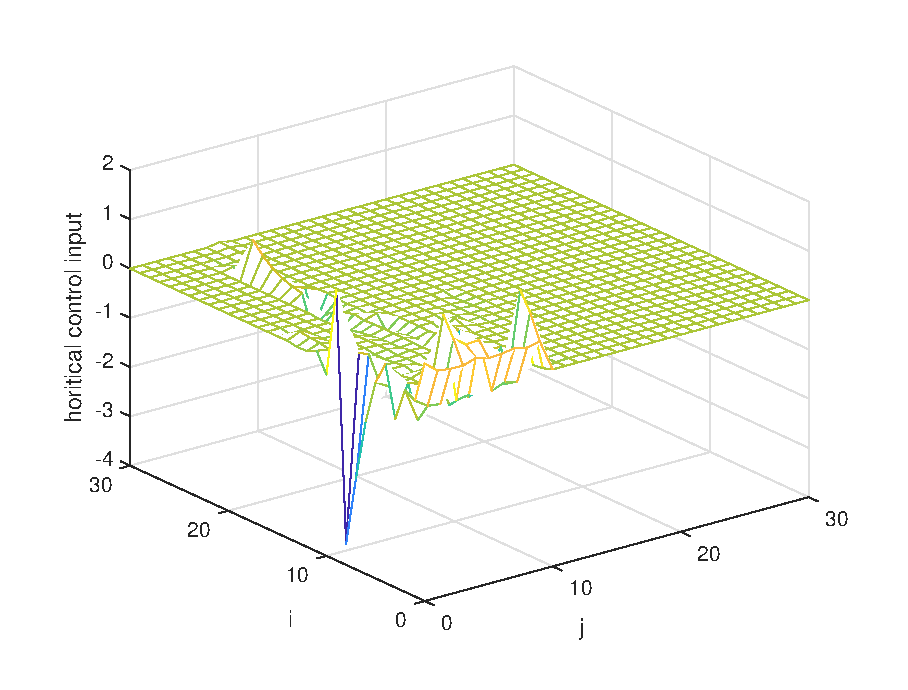
\includegraphics[scale=0.6]{./figures/qc/simulation/hU.eps}\\ 
		\caption{水平控制$u^{v}(i,j)$}
		\label{figqcuh}
	\end{figure}
	
	\begin{figure}[!htb]
		\centering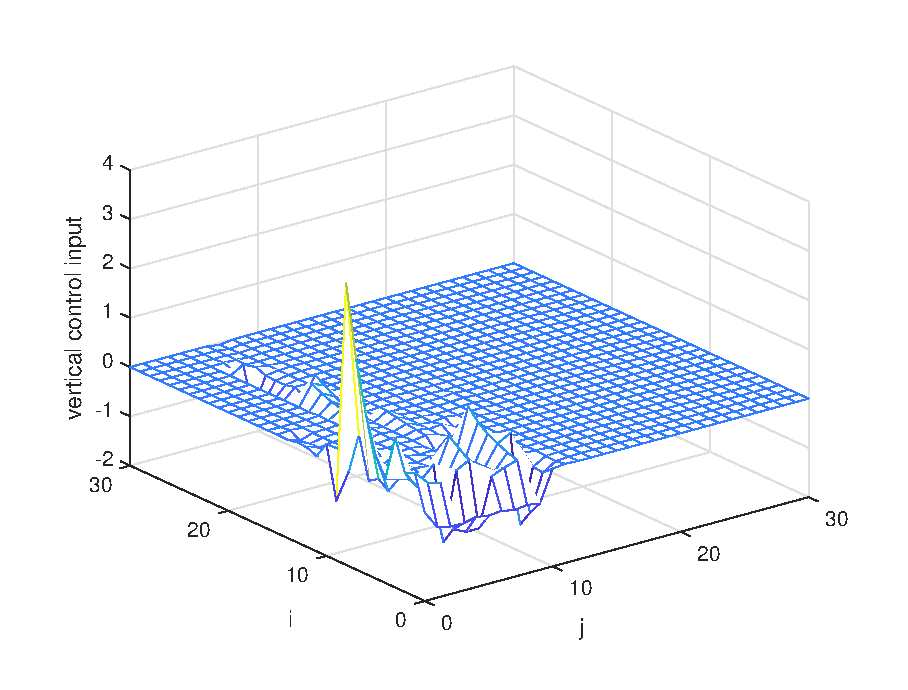
\includegraphics[scale=0.6]{./figures/qc/simulation/vH.eps}\\ 
		\caption{垂直控制$u^{v}(i,j)$}
		\label{figqcuv}
	\end{figure}

\section{小结} \label{conclusion} 	
	本章我们研究了Roesser模型下的二维Markov跳变系统的异步二次型控制问题。考虑到控制器不能获得完整的系统模态信息,存在控制器模态和系统模态不匹配的现象,因此我们基于隐Markov模型设计了异步二次型控制器。借助线性矩阵不等式及李雅普诺夫函数方法,我们对三种不同的初始条件展开了讨论,分别得到了不同情况下的的最优保成本性能。同时,不管初始条件如何,系统都是渐进均方稳定的。
	
	
% !TEX root = ../thesis.tex

\chapter{总结与展望}
	本文主要研究了几类具有不匹配模态Markov跳变系统的异步控制问题。隐Markov模型的引入,可以降低系统对物理装置可靠性及性能的要求,允许控制器模态同系统模态不保持一致,这意味着得到的结果更具有实际应用意义。同时,该基于该模型设计的控制器,可以非常方便的拓展到模态完全匹配及单模态控制器模态不匹配的情况。
	
	本文主要的成果总结如下:
	
	1. 我们讨论了基于模态完全匹配的同步控制器存在的问题和局限性,介绍了隐Markov模型,并说明了基于隐Markov模型来解决模态不完全匹配的异步控制器的优势。
	
	2. 针对一的Markov跳变Lur'e系统,我们引入了隐Markov模型来设计控制器以解决模态不匹配问题。 该控制器由一个由线性状态反馈及同系统非线性保持一致的非线性输出反馈组成,相比单一状态反结构,这样的复合结构创建的控制器要更加灵活,得到的结果也更好。 同时,我们分析了系统的稳定性和$l_2$性能,并用仿真验证了得到结果的有效性。
	
	3.针对一类模态不匹配的Roesser模型表示的非线性2D-Markov跳变系统,我们首先根据2D系统的性质,设计了一个新颖的2D滑模面。然后,考虑到模态不匹配问题,我们根据隐Markov模型和滑模面设计了对应的异步滑模控制器。先是分别讨论了满足一定$H_\infty$性能的系统稳定性问题和系统状态到滑模面的可达性问题,然后又得到了一个可以同时满足两者的充分条件。整个异步滑模控制器的设计步骤被总结成了一个算法,该算法的有效性最终被一个仿真验证。
	
	4.针对一类模态不匹配Rosser模型表示的2D-Markov跳变系统,我们分析了它的异步二次型控制问题。首先根据隐Markov模型,设计了一个异步线性状态反馈控制器,并定义了对应的二次型成本函数。最终我们得到了可以使得系统渐进均方稳定的充分条件,并根据不同的初始条件,分别讨论了他们的最优保成本性能,并使用仿真例子验证了提出方法的有效性。
	
	但是,在研究的过程中,我们也发现了一些可以改进或者需要进一步研究的地方:
	
	1. 2D-Markov 跳变系统的模态传播也存在两个方向。目前的模态传播是基于在水平、垂直方向上满足同一个模态转移概率。在Roesser模型下,同一个坐标包含的水平、垂直两个方向模态,分别来自两个不同的坐标,但是理论上同一个坐标下只应该有一个模态的,如何保证水平、垂直方向的模态一致?
	
	2. 2D系统的初始状态是否存在更好的约束条件?让它更符合实际应用、得到的结果更好、更容易分析。
	
	3. 异步滑模控制是否可以推广到Fornasini-Marchesini模型描述的2D-Markov跳变系统也是一个值得探究的问题。在该模型下,滑模面应该如何构造,控制器应该如何设计值得进一步研究。
%% !TEX root = ../thesis.tex
\chapter{学位论文基本结构}
学位论文基本结构包括前置部份、主体部份和结尾部份\footnote{测试脚注另起一章编号的变化}。
\section{前置部分包括}
\begin{enumerate}
	\item 封面
	\item 题名页
	\item 英文题名页(硕士可省略)
	\item 独创性声明(知识产权声明?)
	\item 勘误表(可根据需要)
	\item 致谢
	\item 序言或前沿(可根据需要)
	\item 摘要页
	\item 目次页
	\item 插图和附表清单(可根据需要)
	\item 缩写、符号清单、术语表(可根据需要)
\end{enumerate}
\section{主体部分}
\begin{enumerate}
	\item 引言(绪论)
	\item 正文
	\item 结论
\end{enumerate}
\section{结尾部分}
\begin{enumerate}
	\item 参考文献
	\item 附录(可根据需要)
	\item 索引(根据需要)
	\item 作者简历及在学期间所取得的科研成果
	\item 封底
\end{enumerate}
\chapter{版面设置}
\section{字体设置}
字体设置
\begin{table}[htb]
	\caption{文章字体设置效果}
	\label{tab:文章字体设置效果}
	\begin{center}
		\begin{tabular}{ccc}
			\toprule
					& 英文字体 & 中文字体  \\
			\midrule
			正文字体 & I can eat glass, it doesn't hurt me. & 我能吞下玻璃而不伤身体 \\
			\textbackslash textrm\{\} & \textrm{I can eat glass, it doesn't hurt me.} & \textrm{我能吞下玻璃而不伤身体} \\
			\textbackslash textsf\{\} & \textsf{I can eat glass.} & \textsf{我能吞下玻璃而不伤身体} \\
			\textbackslash texttt\{\} & \texttt{I can eat glass.} & \texttt{我能吞下玻璃而不伤身体} \\
			\textbackslash textbf\{\} & \textbf{I can eat glass.} & \textbf{我能吞下玻璃而不伤身体} \\
			\bottomrule
		\end{tabular}
	\end{center}
\end{table}

%% !TEX root = ../thesis.tex
\chapter{编写规范与要求}
\section{前置部分}
\subsection{封面}
封面包括分类号、密级、单位代码、作者学号、校名、学校徽标、学位论文中文题目、英文题目、作者姓名、导师姓名、学科和专业名称、提交时间等内容(\textbf{见附件1:学位论文封面样式})。
\subparagraph{分类号} % (fold)
\label{par:分类号}
按中国图书分类法,根据学位论文的研究内容确定。
% subparagraph 分类号 (end)
\subparagraph{密级} % (fold)
\label{par:密级}
仅限于涉密学位论文(论文课题来源于国防军工项目)填写,密级应根据涉密学位论文确定,分绝密、机密和秘密三级,并注明保密期限。非涉密学位论文不得填写密级。
% subparagraph 密级 (end)
\subparagraph{单位代码} % (fold)
\label{par:单位代码}
10335
% subparagraph 单位代码 (end)
\subparagraph{作者学号} % (fold)
\label{par:作者学号}
全日制和在职攻读专业学位者填写学号,同等学力申请学位人员填写申请号。
% subparagraph 作者学号 (end)
\subparagraph{论文题目} % (fold)
\label{par:论文题目}
应准确概括整个论文的核心内容,简明扼要,一般不能超过25个汉字,英文题目翻译应简短准确,一般不应超过150个字母,必要时可以加副标题。
% subparagraph 论文题目 (end)
\subparagraph{学科和专业名称} % (fold)
\label{par:学科和专业名称}
必须按国家研究生培养的学科专业目录,规范填写。
% subparagraph 学科和专业名称 (end)
\subsection{题名页} % (fold)
\label{sub:题名页}
题名页应包括:学位论文中英文题目,学位论文导师及作者本人签名,学位论文评阅人姓名、职称和单位等信息(隐名评阅除外),学位论文答辩委员会主席及成员姓名、职称和单位,学位论文答辩日期等(详见附件2题名页样式)。
% subsection 题名页 (end)
\subsection{英文题名页} % (fold)
\label{sub:英文题名页}
中文题名页相对应的英文翻译。
% subsection 英文题名页 (end)
\subsection{独创性声明} % (fold)
\label{sub:独创性声明}
(见附件3浙江大学研究生学位论文独创性声明)。
% subsection 独创性声明 (end)
\subsection{致谢} % (fold)
\label{sub:致谢}
(见附件3浙江大学研究生学位论文独创性声明)。
% subsection 致谢 (end)
\subsection{序言或前言} % (fold)
\label{sub:序言或前言}
学位论文的序言或前言,一般是作者对本篇论文基本特征的简介,如说明研究工作缘起、背景、主旨、目的、意义、编写体例,以及资助、支持、协作经过等。这些内容也可以在正文引言(绪论)中说明。
% subsection 序言或前言 (end)
\subsection{摘要} % (fold)
\label{sub:摘要}
包括中文摘要和英文摘要两部份。摘要是论文内容的总结概括,应简要说明论文的研究目的、基本研究内容、研究方法、创新性成果及其理论与实际意义,突出论文的创新之处。不宜使用公式、图表,不标注引用文献。硕士论文摘要的字数一般为300--500个左右,博士论文摘要的字数为500-1000个。英文摘要应与中文摘要内容相对应。摘要最后另起一行,列出4—8个关键词。关键词应体现论文特色,具有语义性,在论文中有明确的出处。并应尽量采用《汉语主题词表》或各专业主题词表提供的规范词。
% subsection 摘要 (end)
\subsection{目次页} % (fold)
\label{sub:目次页}
论文中内容标题的集合。包括引言(前言)、章节或大标题的序号和名称、小结、参考文献、注释、索引等,排在序言和前言之后另起页(见附件4目次页样式)。
% subsection 目次页 (end)
\subsection{插图和附表清单} % (fold)
\label{sub:插图和附表清单}
论文中如图表较多,可以分别列出清单置于目次页之后。图的清单应有序号、图题和页码。表的清单应有序号、表题和页码。
% subsection 插图和附表清单 (end)
\subsection{缩写、符号清单和术语表} % (fold)
\label{sub:缩写_符号清单和术语表}
符号、标志、缩略词、首字母缩写、计量单位、术语等的注释表。
% subsection 缩写_符号清单和术语表 (end)
\section{主体部份} % (fold)
\label{sec:主体部份}
包括引言(绪论)、正文和结论。主体部分应从另页右页开始,每一章应另起页。
\subsection{一般要求} % (fold)
\label{sub:一般要求}
\subsubsection{引言(绪论)} % (fold)
\label{ssub:引言_绪论_}
应包括论文的研究目的,流程和方法等。论文研究领域的历史回顾,文献回溯,理论分析等内容,应独立成章,用足够的文字叙述。
% subsubsection 引言_绪论_ (end)
\subsubsection{正文} % (fold)
\label{ssub:正文}
主体部分由于涉及不同的学科,在选题、研究方法、结果表达方式等有很大的差异,不能作统一的规定。但是,论文应层次分明、数据可靠、图表规范、文字简炼、说明透彻、推理严谨、立论正确,避免使用文学性质的带感情色彩的非学术性词语。论文中如出现非通用性的新名词、新术语、新概念,应作相应解释。
\subparagraph{图} % (fold)
\label{subp:图}
图应具有“自明性”。图包括曲线图、构造图、示意图、框图、流程图、记录图、地图、照片等,应鲜明清晰。照片上应有表示目的物尺寸的标度。图的编号和图题规范,并应置于图下方。
% subparagraph 图 (end)
\subparagraph{表} % (fold)
\label{subp:表}
表应具有“自明性”。表的编号和表题规范,并置于表上方。表题应简单明了。
表的编排,一般是内容和测试项目由左至右横读,数据依序竖读。如某个表需要转页接排,在随后的各页上应重复表的编号。编号后跟表题(可省略)和“(续)”,置于表上方。续表均应重复表头。
% subparagraph 表 (end)
\subparagraph{公式} % (fold)
\label{subp:公式}
论文中的公式应另行起,并缩格书写,与周围文字留足够的空间区分开。如有两个以上的公式,应用从“1”开始的阿拉伯数字进行编号,并将编号置于括号内。公式的编号右端对齐,公式与编号之间可用“…”连接。公式较多时,应分章编号。较长的公式需要转行时,应尽可能在“=”处回行,或者在“+”、“-”“×”、“/”等记号处回行。
% subparagraph 公式 (end)
\subparagraph{引文标注} % (fold)
\label{subp:引文标注}
论文中引用的文献的标注方法遵照GB/T 7714-2005,可采用顺序编码制,也可采用著者-出版年制,但全文必须统一。如:

德国学者N.克罗斯研究了瑞士巴塞尔市附近侏罗山中老第三纪断裂对第三系摺皱的控制[25];之后,他又描述了西里西亚第3条大型的近南北向构造带,并提出地槽是在不均一的块体的基底上发展的思想[26] 。(顺序编码制)

结构分析的子结构法最早是为解决飞机结构这类大型和复杂结构的有限元分析问题而发展起来的(Przemienicki,1968)(著者-出版年制)
% subparagraph 引文标注 (end)
\subparagraph{注释} % (fold)
\label{subp:注释}
当论文中的字、词或短语,需要进一步加以说明,而又没有具体的文献来源时,用注释。注释一般在社会科学中用得较多。应控制论文中的注释数量,不宜过多。注释采用文中编号加“脚注”的方式,置于当页的页脚。
% subparagraph 注释 (end)
% subsubsection 正文 (end)
% subsection 一般要求 (end)
\subsection{章节图表标号规则} % (fold)
\label{sub:章节图表标号规则}
\subsubsection{章节标号} % (fold)
\label{ssub:章节标号}
论文章节按序分层。层次以少为宜,根据实际需要选择。各层次标题一律用阿拉伯数字连续标号;不同层次的数字之间用小圆点“.”相隔,末位数字后面不加点号,如“1”,“1.1”,“1.1.1”等;章、节编号全部顶格排,编号与标题之间空1个字的间隙。章的标题占2行。正文另起行,前空2个字起排,回行时顶格排。例如:
\begin{verbatim}
1 ××××(章大标题),
×××××××××××××××××××××××××××
1.1 ××××(一级节标题)
1.1.1 ××××(二级节标题)
1.1.1.1 ××××(根据需要,也可设三级节标题)
2 ××××(章大标题)
2.1 ××××(一级节标题)
2.1.1 ××××(二级节标题)
\end{verbatim}
% subsubsection 章节标号 (end)
\subsubsection{图、表等标号} % (fold)
\label{ssub:图_表等标号}
论文中的图、表、附注、公式、算式等,一律用阿拉伯数字分章依序连续编码。其标注形式应便于互相区别,如:图 l.1(第1章第一个图)、图2.2(第二章第二个图);表3.2(第三章第二个表)等。
% subsubsection 图_表等标号 (end)
\subsubsection{页码、页眉编写规则} % (fold)
\label{ssub:页码_页眉编写规则}
学位论文的页码,前置部分用罗马数字单独编连续码,正文和后置部分用阿拉伯数字编连续码。单面复印时页码排在页脚居中位置,双面复印时页码分别按左右侧排列。

页眉、页脚文字均采用小五号宋体,左侧页眉为“浙江大学博(硕)士学位论文”,右侧为一级标题名称;页眉下横线可为单横线也可用上粗下细文武线。
% subsubsection 页码_页眉编写规则 (end)
% subsection 章节图表标号规则 (end)
\subsection{结论} % (fold)
\label{sub:结论}
论文的结论是最终的、总体的结论,不是正文中各段的小结的简单重复。结论应包括论文的核心观点,交代研究工作的局限,提出未来工作的意见或建议。结论应该准确、完整、明确、精练。

如果不能导出一定的结论,也可以没有结论而进行必要的讨论。
% subsection 结论 (end)
% section 主体部份 (end)
\section{结尾部分} % (fold)
\label{sec:结尾部分}
\subsection{参考文献} % (fold)
\label{sub:参考文献}
参考文献表是文中引用的有具体文字来源的文献集合,其著录项目和著录格式遵照GB/T 7714-2005的规定执行。

参考文献表应置于正文后,并另起页。所有被引用文献均要列入参考文献表中。引文采用顺序编码标注时,参考文献表按编码顺序排列,引文采用著作-出版年制标注时,参考文献表应按著者字顺和出版年排序。

各种主要参考文献按如下格式编排:

学术期刊:序号 作者 文题 刊名 年 卷号(期号) 起止页码

专(译)著:序号 作者(译者) 书名. 出版地:出版者,出版年,起止页码

学位论文:序号 作者 文题 [XX学位论文] 授予单位所在地 授予单位 授予年份  起止页码

专利:序号 申请者 专利名 国名 专利文献种类 专利号 出版日期

技术标准:序号 发布单位 技术标准代号 技术标准名称 出版地:出版者,出版日期

电子文献:序号 作者 出版年 题名 出版地 出版者 [引用日期] 获取和访问路径
% subsection 参考文献 (end)
\subsection{附录} % (fold)
\label{sub:附录}
附录作为主体部分的补充,并不是必须的。

下列内容可以作为附录编于论文后。

为了整篇论文材料的完整,但编入正文又有损于编排的条理性和逻辑性,这一材料包括比正文更为详尽的信息、研究方法和技术更深入的叙述,对了解正文内容有用的补充信息等。

由于篇幅过大或取材于复制品而不便于编入正文的材料。

不便于编入正文的罕见珍贵资料。

对一般读者并非必要阅读,但对本专业同行有参考价值的资料。

某些重要的原始数据、数学推导、结构图、统计表、计算机打印输出件等。
% subsection 附录 (end)
\subsection{索引} % (fold)
\label{sub:索引}
根据需要可以编排分类索引,关键词索引等。
% subsection 索引 (end)
\subsection{作者简历} % (fold)
\label{sub:作者简历}
包括教育经历、工作经历、攻读学位期间发表的论文和完成的工作等。
% subsection 作者简历 (end)
% section 结尾部分 (end)

\backmatter
\bibliography{reference_data_base/references}
% \nocite{*} % to show the entire references, annotate it if need.
%\appendix
%% !TEX root = ../thesis.tex
\chapter{我是第一个附录}
\section{我是第一个附录的第一节}
这是一个附录测试页,内容无关紧要。\footnote{以下内容引用自《三体:黑暗森林》}以%
下段落较长,以防数组溢出,故采用回车强制分行处理。分行出换行符在\TeX 中算作一个%
空格,因此,在每段后加注释符。不过在中文环境中换行加不加注释符都不会产生空格,不%
过还是加上吧。

罗辑抬起左手,露出了戴在手腕上的手表大小的东西说:“这是一个生命体征监测仪,它通%
过一个发射器与一套摇篮系统联结。你们一定记得两个世纪前面壁者雷迪亚兹的事,那就一%
定知道摇篮系统是什么。这个监测仪所发出的信号通过摇篮系统的链路,到达雪地工程部署%
在太阳轨道上的三千六百一十四枚核弹。

信号每秒钟发射一次,维持着这些核弹的非触发状态。如果我死去,摇篮系统的维持信号将%
消失,所有的核弹将被引爆,包裹核弹的油膜物质将在爆炸中形成围绕太阳的三千六百一十%
四团星际尘埃,从远方观察,在这些尘埃云团的遮挡下,太阳将在可见光和其他高频渡段发%
生闪烁。太阳轨道上所有核弹的位置都是经过精心布置的,使得太阳闪烁形成的信号发送出%
三张简单的图形,就像我两个世纪前发出的那三张图一样,每张上面有三十个点的排列,并%
标注其中一个点,它们可以组合成一个三维坐标图。但与那次不同的是,这次发送的,是三%
体世界与周围三十颗恒星的相对位置。太阳将变成银河系中的一座灯塔,把这咒语发送出去%
,当然,太阳系和地球的位置也会同时暴露。从银河系中的一点看,图形发射完成需要一年%
多的时间,但应该有很多技术发展到这样程度的文明,可以从多个方向同时观测太阳,那样%
的话,只需几天甚至几个小时,他们就能得到全部信息。”

\section{数学模式测试}
这里用于测试附录部分的数学公式,诸如标号,交叉应用等。

交叉引用测试,如交引用命令{\ttfamily \textbackslash eqref}和\texttt{\textbackslash ref}命令的区别。如公式\eqref{eq:apptest1},\autoref{eq:apptest1}显示,\texttt{\textbackslash eqref}命令比\texttt{\textbackslash ref}命令的应用结果多了个括号。

如公式\eqref{eq:apptest3}是单行公式环境,查看公式\eqref{eq:apptest3}和\eqref{eq:apptest1}之间的区别,好像在单行公式中没什么区别。
\begin{align}\label{eq:apptest3}
	f(x) = 2(x + 1)^{2} - 1
\end{align}

\texttt{align}公式环境,用在单行中。
\begin{align}\label{eq:apptest1}
	f(x) = 2(x + 1)^{2} - 1
\end{align}

在这里,中间插入一些文字以形成段落,查看行间公式与上下文之间的间隙。
\begin{align*}
	f(x) = 2(x + 1)^{2} - 1
\end{align*}
在这里,中间插入一些文字以形成段落,查看行间公式与上下文之间的间隙。下一个公式\eqref{eq:apptest2}是一个公式组,它在“=”位置对齐。
\begin{align}\label{eq:apptest2}
	f(x) & = 2(x + 1)^{2} - 1\\
		 & = 2(x^{2} + 2x +1)-1\\
		 & = 2x^{2} + 4x + 1
\end{align}

\subsection{我是第一个附录的第二节的第一个子节}

\section{表格测试}
在这里推荐制表采用功能强大的tabu宏包以取代其它制表宏包。具体tabu宏包的使用说明参见tabu宏包的说明文档。

以下节分别用来测试各种表格环境如,tabular,tabu,longtabu等,还有对caption格式的修改和测试。以下表格样式全部采用三线表。

\subsection{array宏包tabular表格环境测试}
如\autoref{tab:appfirst_table_test}是对array宏包的tabular表格环境测试。
\begin{table}[htbp]
	\centering
	\caption{这是一个用tabular环境的测试用的表格}\label{tab:appfirst_table_test}
    \begin{tabular}{lrr}
    \toprule
    \textbf{行星}     & \textbf{赤道半径}km & \textbf{公转周期}d \\
    \midrule
    水星     & 2.439  & 87.9 \\
    金星     & 6.1    & 224.682 \\
    地球     & 6378.14 & 365.24 \\
    \bottomrule
    \end{tabular}%
\end{table}

\subsection{tabu宏包表格环境测试}
如\autoref{tab:apptabu_test_1}是对tabu宏包的tabu表格环境测试。在这里表格命令与\autoref{tab:appfirst_table_test}的命令相同,只是tabular环境改成了tabu环境。
\begin{table}[htbp]
	\centering
	\caption{这是一个用tabu环境的测试用的表格}\label{tab:apptabu_test_1}
    \begin{tabu}{lrr}
    \toprule
    \textbf{行星}     & \textbf{赤道半径}km & \textbf{公转周期}d \\
    \midrule
    水星     & 2.439  & 87.9 \\
    金星     & 6.1    & 224.682 \\
    地球     & 6378.14 & 365.24 \\
    \bottomrule
    \end{tabu}%
\end{table}

\section{插图测试}
如\autoref{fig:appfirst_image_tset}是对此模版的第一张插图测试。

\begin{figure}[htbp]
	\centering
	
\includegraphics[width = 0.5\linewidth]{Chapter8.png}
	\caption{附录页第一张插图测试}\label{fig:appfirst_image_tset}
\end{figure}

\section{我是第一个附录的第五节}
随着天光渐明,星星在一颗颗消失,仿佛无数只眼睛渐次闭上;而东方正在亮起的晨空,则%
像一只巨大的眼睛在慢慢睁开。蚂蚁继续在叶文洁的墓碑上攀爬着,穿行在她的名字构成的%
迷宫中。早在这个靠碑而立的豪赌者出现前的一亿年,它的种族已经生活在地球上,这个世%
界有它的一份,但对正在发生的事,它并不在意。

罗辑离开墓碑,站到他为自己挖掘的墓穴旁,将手枪顶到自己的心脏位置,说:“现在,我
将让自己的心脏停止跳动,与此同时我也将成为两个世界有史以来最大的罪犯。对于所犯下
的罪行,我对两个文明表示深深的歉意,但不会忏悔,因为这是唯一的选择。我知道智子就
在身边,但你们对人类的呼唤从不理睬,无言是最大的轻蔑,我们忍受这种轻蔑已经两个世
纪了,现在,如果你们愿意,可以继续保持沉默,我只给你们三十秒钟时间。”罗辑按照自
己的心跳来计时,由于现在心跳很急促。他把两次算一秒钟,在极度的紧张中他一开始就数
错了,只好从头数起,所以当智子出现时他并不能确定到底过了多少时间,客观时间大约流
逝了不到十秒钟,主观时间长得像一生。

这时他看到世界在眼前分成了四份,一份是周围的现实世界,另外三份是变形的映像。映像%
来自他前上方突然出现的三个球体,它们都有着全反射的镜面,就像他在最后一个梦中见到%
的墓碑那样。他不知道这是智子的几维展开,那三个球体都很大,在他的前方遮住了半个天%
空,挡住了正在亮起来的东方天际,在球体中映出的西方天空中他看到了几颗残星,球体下%
方映着变形的墓地和自己。罗辑最想知道的是为什么是三个,他首先想到的是三体世界的象%
征,就像叶文洁在最后一次ETO的聚会上看到的那个艺术品:但看到球体上所映照的虽然变%
形但异常清晰的现实图像时,他又感觉那是三个平行世界的入口,暗示着三种可能的选择;

%% !TEX root = ../thesis.tex
\chapter{我是第二个附录}
\section{我是第二个附录的第一节}
这是一个附录测试页,内容无关紧要。\footnote{以下内容引用自《三体:死神永生》}

这时。“蓝色空间”号和“万有引力”号同时停止前进,并后退了三十万千米,因为“魔戒”进入%
三维太空时,在维度跌落过程中将放出巨大的能量,这也是之前出现的那些长线发光的原因。%

二十二天后,四维碎块的边界退过了“魔戒”。在它进入三维太空的那一瞬间,宇宙仿佛被拦%
腰斩断,长长的断口发出炫目的强光,如同一颗恒星被瞬间拉成一条线。当光芒黯淡一些后%
,一条横过整个太空的长线显现出来,从飞船上看不到它的头和尾,像上帝在宇宙的绘图板%
上比着丁字尺从左到右画了一道。据测量,这条把可见的宇宙分成两部分的线,其长度接近%
一个天文单位。约一亿三千万千米,几乎可以把地球和太阳连接起来。与以前出现的那些长%
线不同,这条线即使从几十万千米外仍能看出其宽度。长线发出的光由蓝白变成红色,然后%
渐渐暗淡下去,线本身也变得宽散弯曲。由一条笔直的长线变成一道尘埃带,弯弯曲曲不见%
首尾。它自身己经不发光,但浸透了星海的光芒,变成宁静的银灰色。两艘飞船上观看的人%
们这时都有一个奇怪的印象,感觉尘埃带看上去很像宇宙背景上的银河系,刚才发生的仿佛%
是一次对银河系的宏大摄影,闪光灯闪过后,拍下的照片在太空中渐渐显影。

看着这壮丽的景象,关一帆有些伤感,他想起了自己送给“魔戒”的生态球,它只拥有了那个%
礼物不长的时间。在三维展开的一刹那,“魔戒”内部的所有四维结构都被完全破坏,这是一%
场最彻底的毁灭。四维碎块中其他那些已经死去或仍活着的飞船,最终也都无法逃脱这样的%
命运,在这广阔的宇宙中,它们只能在四维碎块这个小小的角落中存在。

一个巨大而黑暗的秘密。

“蓝色空间”号和“万有引力”号派出多艘太空艇前往尘埃带,除了考察外,还想看看能不能收%
集一些有用的资源。“魔戒”三维化以后都变成很普通的元素,大部分是氢和氮,从中有可能%
得到核聚变燃料。但尘埃中的这两种元素都呈气态,扩散很快,没有收集到多少。另外还有%
一些重元素。可以采集到一些有用的金属。

现在,两艘飞船应该考虑自己的未来了。由“蓝色空间”号和“万有引力”号共同组成的一个临%
时委员会宣布,两艘飞船上的任何人都可以做出选择:随两舰继续航行或返回太阳系。两舰%
将装配一个独立于两舰的冬眠舱,并把两舰上七台聚变发动机中的一台用于推进它,决定返%
回的人将乘坐这艘临时装配的飞船,在冬眠中返回太阳系,航行时问预计为三十五年。两舰%
将用中微子通信通知地球冬眠飞船的轨道参数,以便在它到达太阳系时进行接应。为了防止%
三体世界借此侦测到两舰的位置,与地球的联系将在冬眠飞船起航一段时间后再进行。如果%
地球方面能够在飞船到达太阳系前派出接应飞船协助减速的话,加速段就有更多的燃料用于%
推进,返回的航程可以缩短至十几年。

如果那时还有太阳系和地球的话。

只有两百多人选择返回,其余的人不想回到那个正在走向毁灭的世界,决定随“蓝色空间”号%
和“万有引力”号继续航行,飞向未知的太空深处。

\subsection{我是第二个附录的第一节的第一个子节}
\subsubsection{我是第二个附录的第一节的第一个子节的第一个子子节}

\end{document}